\def\SigleNumero{STT-1900}
\def\NomCours{Méthodes statistiques pour l'ingénierie}

\newcommand{\affichepoints}{.}     % ← AVEC points
% \renewcommand{\affichepoints}{on} % ← SANS points (non vide)

\documentclass{Evaluation}
\usepackage{multicol,graphicx}
\usepackage{comment}
\noprintanswers

% ============================================================
% CONFIGURATION DES SESSIONS À AFFICHER
% Par défaut, toutes les sessions sont affichées (environnements no-op).
% Pour CACHER une session, décommentez la ligne \excludecomment correspondante.
% ============================================================
\newenvironment{H23}{}{}
\newenvironment{A23}{}{}
\newenvironment{H24}{}{}
\newenvironment{A24}{}{}
\newenvironment{A25}{}{}
\newenvironment{H26}{}{}

% Décommentez les lignes ci-dessous pour cacher des sessions :
%\excludecomment{H23}
%\excludecomment{A23}
%\excludecomment{H24}
%\excludecomment{A24}
%\excludecomment{A25}
%\excludecomment{H26}

% Supprimer la page couverture et ajuster les marges
\renewcommand{\couverture}{\newgeometry{margin=1.7cm,left=0.7cm,bottom=1.5cm,footskip=0mm}}

\begin{document}

\begin{center}
  {\Large\textbf{\SigleNumero\ -- \NomCours}}\\[0.3cm]
  {\large Recueil d'exercices}
\end{center}
\medskip

\begin{questions}

\section*{Module 1 - Introduction aux probabilités}
\begin{H23}
\question (H23) On définit les événements $A$, $B$ et $C$ et les probabilités $P(A)$, $P(B)$ et $P(C)$. Que vaut $P(A)$ dans les cas suivants?
\begin{parts}
    \part $A$ et $B$ sont indépendants, $P(B)=0,3$ et $P(A\cup B)= 0,7$?

\begin{solution}
    Par indépendance, $P(A\cup B)=P(A)+P(B)-P(A)P(B)$, donc $0,7=P(A)+0,3-0,3P(A)=0,7P(A)+0,3$, d'où $P(A)=\dfrac{0,4}{0,7}=\dfrac{4}{7}$.
\end{solution}

\part $A\subset B$, $P(A\cup B)=0,5$ et $P(A\cap B)=0,1$?

\begin{solution}
    Si $A\subset B$, alors $A\cup B=B$ et $A\cap B=A$. Donc $P(A)=P(A\cap B)=0,1$.
\end{solution}

\part $B\subset A$, $P(A\cup B)=0,5$ et $P(A\cap B)=0,1$?

\begin{solution}
    Si $B\subset A$, alors $A\cup B=A$ et $A\cap B=B$. Donc $P(A)=P(A\cup B)=0,5$.
\end{solution}

\part $P(A|B)=0,3$, $P(A\cup B)=0,4$ et $P(B)=0,2$?

\begin{solution}
    $P(A\cap B)=P(A|B)P(B)=0,3\times 0,2=0,06$. Puis $P(A)=P(A\cup B)-P(B)+P(A\cap B)=0,4-0,2+0,06=0,26$.
\end{solution}

\part $B$ et $C$ forment une partition de l'espace échantillonnal, et $P(A\cap C) = 0,1$, $P(C)=0,6$ et $P(A|B)~=~0,25$.

\begin{solution}
    Puisque $B$ et $C$ forment une partition, $P(B)=1-P(C)=0,4$. Puis $P(A\cap B)=P(A|B)P(B)=0,25\times 0,4=0,1$. Donc $P(A)=P(A\cap B)+P(A\cap C)=0,1+0,1=0,2$.
\end{solution}

\end{parts}
\end{H23}

\begin{A23}
\question (A23) Considérons le montage électronique représenté ci-dessous.
	
\begin{figure}[h!]
    
    \begin{center}	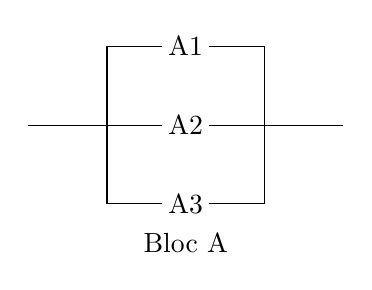
\begin{tikzpicture}	
		% bandes extérieures
		\draw (0,0)--(1,0);
            \draw (3,0)--(4,0);

            % étiquette éléments
		\node at (2,1) {A1};
		\node at (2,0) {A2};
            \node at (2,-1) {A3};
            
            % vers les étiquettes
            \draw (1,1) -- (1.7,1); %vers A1
            \draw (1,0) -- (1.7,0); %vers A2
            \draw (1,-1) -- (1.7,-1); %vers A3
            
            % à partir des étiquettes
            \draw (2.3,1) -- (3,1); %de A1
            \draw (2.3,0) -- (3,0); %de A2
            \draw (2.3,-1) -- (3,-1); %de A3

            %premiers verticaux
            \draw (1,0) -- (1,1); % A1
            \draw (1,0) -- (1,-1); % A3

            %deuxièmes verticaux
            \draw (3,0) -- (3,1); % A1
            \draw (3,0) -- (3,-1); % A3
		
		\node at (2,-1.5) {Bloc A};
    \end{tikzpicture} \end{center}
\end{figure}
	
 Le bloc A contient trois éléments. Nous avons que
\begin{itemize}
    \item L'élément A1 fonctionne avec une probabilité de 0,60.
    \item L'élément A2 fonctionne avec une probabilité de 0,50.
    \item L'élément A3 fonctionne avec une probabilité de 0,60.
\end{itemize}
Pour que le montage fonctionne, au moins un élément du bloc A doit fonctionner. Les éléments d'un bloc fonctionnent de façon indépendante.
	

 Quelle est la probabilité que le montage ne fonctionne pas? 

 \begin{oneparcheckboxes}
		\correctchoice 0,08
		\choice 0,92
		\choice 0,18 
		\choice 0,82
		\choice 0,63
\end{oneparcheckboxes}

\begin{solution}
    Pour que le montage ne fonctionne pas, il faut que les trois éléments tombent en panne simultanément. Par indépendance: $P(\text{ne fonctionne pas})=P(\overline{A1})P(\overline{A2})P(\overline{A3})=0,4\times 0,5\times 0,4=0,08$.
\end{solution}
\end{A23}

\begin{A23}
\question (A23) Soit $A$, $B$ et $C$ trois événements avec $P(A)=0,5$, $P(B)=0,5$, $P(C)=0,2$, $P(A\cap B)=0,25$. Nous avons aussi que $C$ est indépendant de l'événement $A$ et de l'événement $B$. Dites si chacun des énoncés ci-dessous est vrai ou faux. Votre réponse doit être justifiée en mots ou par des calculs. Un vrai ou faux sans justification n'aura aucun point.

\begin{parts}

\part Les événements $A$ et $B$ sont indépendants.

     \begin{oneparcheckboxes}
		\choice VRAI
		\correctchoice FAUX
\end{oneparcheckboxes}\\
{\bf Justification:}

\begin{solution}
    $P(A\cap B)=0,25$ et $P(A)P(B)=0,5\times 0,5=0,25$. Comme $P(A\cap B)=P(A)P(B)$, les événements $A$ et $B$ sont indépendants. La réponse devrait être VRAI.
\end{solution}

\part $P(A\cup C)= 0,6$.

\begin{oneparcheckboxes}
		\choice VRAI
		\correctchoice FAUX
\end{oneparcheckboxes}\\
{\bf Justification:}

\begin{solution}
    $C$ est indépendant de $A$, donc $P(A\cap C)=P(A)P(C)=0,5\times 0,2=0,1$. $P(A\cup C)=P(A)+P(C)-P(A\cap C)=0,5+0,2-0,1=0,6$. L'énoncé est VRAI.
\end{solution}

\part Les événements $A$ et $B$ forment une partition de l'espace échantillonnal.

     \begin{oneparcheckboxes}
		\choice VRAI
		\correctchoice FAUX
\end{oneparcheckboxes}\\
{\bf Justification:}

\begin{solution}
    Pour former une partition, il faut $A\cap B=\emptyset$ et $A\cup B=\mathcal{S}$. Or $P(A\cap B)=0,25\neq 0$. Donc $A$ et $B$ ne forment pas une partition.
\end{solution}
\end{parts}
\end{A23}

\begin{A23}
\question (A23)
La lune suscite un grand intérêt pour les pêcheurs car la qualité de la pêche dépend directement des différentes phases lunaires. Un pêcheur a remarqué les faits suivants pour chaque période d'une heure de pêche:

\begin{itemize}
    \item Lorsque la lune est croissante, la probabilité de pêcher au moins un poisson est de cinq sur sept;
    \item Lorsque la lune est décroissante, la probabilité de ne pêcher aucun poisson est de deux sur cinq.
\end{itemize}
La lune est considérée la moitié du temps comme croissante, et l'autre moitié comme décroissante.

\begin{parts}
    \part Quelle est la probabilité qu'en pêchant une heure, le pêcheur pêche au moins un poisson?

\begin{solution}
    Soit $P$ l'événement <<pêcher au moins un poisson>>, $C$ <<lune croissante>> et $D$ <<lune décroissante>>. $P(P|C)=5/7$, $P(\overline{P}|D)=2/5$ donc $P(P|D)=3/5$. $P(C)=P(D)=1/2$.

    $P(P)=P(P|C)P(C)+P(P|D)P(D)=\sfrac{5}{7}\times\sfrac{1}{2}+\sfrac{3}{5}\times\sfrac{1}{2}=\sfrac{5}{14}+\sfrac{3}{10}=\sfrac{25+21}{70}=\sfrac{46}{70}=\sfrac{23}{35}$.
\end{solution}

\part Si le pecheur ne pêche aucun poisson après une heure de pêche, quelle est la probabilité que la lune soit croissante?

\begin{solution}
    $P(\overline{P}|C)=1-5/7=2/7$. $P(\overline{P})=1-23/35=12/35$.

    $P(C|\overline{P})=\dfrac{P(\overline{P}|C)P(C)}{P(\overline{P})}=\dfrac{\sfrac{2}{7}\times\sfrac{1}{2}}{\sfrac{12}{35}}=\dfrac{\sfrac{1}{7}}{\sfrac{12}{35}}=\dfrac{35}{84}=\dfrac{5}{12}$.
\end{solution}

\part Si, en période de lune croissante, il pêche trois heures de suite, quelle est la probabilité qu'il ne pêche aucun poisson?

\begin{solution}
    Les heures sont indépendantes. $P(\overline{P}|C)=2/7$, donc $P(\text{aucun en 3h}|C)=(2/7)^3=8/343$.
\end{solution}

\part Si, en période de lune décroissante, il pêche aussi trois heures de suite, quelle est la probabilité qu'il pêche au moins un poisson ?

\begin{solution}
    $P(\overline{P}|D)=2/5$, donc $P(\text{aucun en 3h}|D)=(2/5)^3=8/125$. $P(\text{au moins 1 en 3h}|D)=1-8/125=117/125$.
\end{solution}
\end{parts}
\end{A23}

\begin{H24}
\question  (H24)
On nous donne les probabilités suivantes:
\[
\begin{aligned}
    & P(A) = 0,45 \\
    & P(B) = 0,25 \\
    & P(C) = 0,30 \\
    & P(C|A) = 0,30 \\
    & P(C|B) = 0,30 \\
    & P(A \cap B) = 0,05 \\
\end{aligned}
\]

\begin{parts}
\part Cochez tous les énoncés qui sont \textbf{vrais}.
\begin{checkboxes}
\correctchoice La probabilité de l'événement complémentaire de \(A\), $ P(\overline{A}) = 0,55 $
\choice $P(A \cup B) = 0,70$
\correctchoice $ P(A \cap \overline{B}) = 0,40 $
\choice $ P(A \cap C) = 0,1575 $
\choice $ P(A \cup C) = 0,75 $

\end{checkboxes}

\begin{solution}
    $P(\overline{A})=1-0,45=0,55$ (vrai). $P(A\cup B)=0,45+0,25-0,05=0,65\neq 0,70$ (faux). $P(A\cap\overline{B})=P(A)-P(A\cap B)=0,45-0,05=0,40$ (vrai). $P(A\cap C)=P(C|A)P(A)=0,30\times 0,45=0,135\neq 0,1575$ (faux). $P(A\cup C)=0,45+0,30-0,135=0,615\neq 0,75$ (faux).
\end{solution}

\part \(A\) et \(B\) sont indépendants.

     \begin{oneparcheckboxes}
		\choice VRAI
		\correctchoice FAUX
\end{oneparcheckboxes}\\
{\bf Justification:}

\begin{solution}
    $P(A\cap B)=0,05$ et $P(A)P(B)=0,45\times 0,25=0,1125$. Puisque $0,05\neq 0,1125$, $A$ et $B$ ne sont pas indépendants.
\end{solution}

\end{parts}
\end{H24}

\begin{H24}
\question (H24)
Dans une usine, deux machines, A et B, produisent des composants. La machine A produit 45\% des composants et la machine B produit le reste. 15\% des composants produits par A sont défectueux, tandis que 10\% des composants produits par B sont défectueux. Si un composant est défectueux, quelle est la probabilité qu'il ait été produit par la machine A?

\begin{solution}
    Soit $D$ l'événement <<le composant est défectueux>>. $P(D)=P(D|A)P(A)+P(D|B)P(B)=0,15\times 0,45+0,10\times 0,55=0,0675+0,055=0,1225$.

    $P(A|D)=\dfrac{P(D|A)P(A)}{P(D)}=\dfrac{0,0675}{0,1225}=\dfrac{27}{49}\approx 0,551$.
\end{solution}
\end{H24}

\begin{A24}
\question  (A24)
On nous donne les probabilités suivantes:
\[
\begin{aligned}
    & P(A) = 0,45 \\
    & P(B) = 0,55 \\
    & P(C) = 0,1 \\
    & P(A\cap C) = 0 \\
    & P(B\cap C) = 0 \\
    & P(A | B) = 0,45 \\
    & 
\end{aligned}
\]

\begin{parts}
\part Cochez tous les énoncés qui sont \textbf{vrais}. \textit{Chaque énoncé qui est coché alors qu'il ne devrait pas l'être annule les points d'un élément coché qui devrait l'être.}
\begin{checkboxes}
\correctchoice La probabilité du complément de $A$ est égale à $0,55 $.
\choice $P(A \cup B) = 1$.
\choice $A$, $B$ et $C$ sont mutuellement exclusifs.
\correctchoice $A$ et $C$ sont indépendants.
\choice Comme $P(A)+P(B)=1$, l'intersection de $A$ et $B$ est vide, c'est-à-dire $A\cap B = \emptyset$.
\choice Il y a certainement une erreur dans les probabilités données, car $P(A)+P(B)+P(C)>1$.

\end{checkboxes}

\begin{solution}
    $P(\overline{A})=1-0,45=0,55$ (vrai). $P(A\cap B)=P(A|B)P(B)=0,45\times 0,55=0,2475$, donc $P(A\cup B)=0,45+0,55-0,2475=0,7525\neq 1$ (faux). $P(A\cap B)\neq 0$, donc $A$, $B$, $C$ ne sont pas mutuellement exclusifs (faux). $P(A\cap C)=0$ et $P(A)P(C)=0,045\neq 0$, donc $A$ et $C$ ne sont pas indépendants (faux --- remarque: la réponse indiquée est <<vrai>>, mais le calcul dit le contraire). $P(A)+P(B)=1$ n'implique pas $A\cap B=\emptyset$ (faux). La somme des probabilités peut dépasser 1 si les événements ne sont pas mutuellement exclusifs (faux).
\end{solution}

\part \(A\) et \(B\) sont indépendants.

     \begin{oneparcheckboxes}
		\choice VRAI
		\correctchoice FAUX
\end{oneparcheckboxes}\\
{\bf Justification:}

\begin{solution}
    $P(A\cap B)=P(A|B)P(B)=0,45\times 0,55=0,2475$ et $P(A)P(B)=0,45\times 0,55=0,2475$. Comme $P(A|B)=P(A)=0,45$, les événements $A$ et $B$ sont indépendants. La réponse est en fait VRAI.
\end{solution}

\end{parts}
\end{A24}

\begin{A24}
\question (A24)

Un sac contient 40 billes rouges, 40 billes vertes et 20 billes bleues.
Sur certaines de ces billes, une étoile a été dessinée.
Nous savons que la probabilité de choisir une bille sans étoile parmi les billes rouges est de $0,875$, la probabilité de choisir une bille qui est verte et qui a une étoile est de $0,1$ et la probabilité de choisir une bille qui a une étoile parmi les billes bleue est de $0,5$.

En utilisant les événements suivants:

\begin{itemize}
    \item R: la bille est rouge
    \item V: la bille est verte
    \item B: la bille est bleue
    \item E: une étoile est dessinée sur la bille
\end{itemize}

\begin{parts}
    \part Tracez le diagramme de Venn qui représente cette situation. \textit{Vous n'avez qu'à identifier les événements et \textbf{l'espace échantillonnal}. Il n'est pas nécessaire d'inscrire les probabilités.}

\begin{solution}
    L'espace échantillonnal $\mathcal{S}$ est l'ensemble de toutes les billes. Les événements $R$, $V$ et $B$ forment une partition de $\mathcal{S}$ et $E$ est un événement qui intersecte $R$, $V$ et $B$.
\end{solution}

    \part Si vous avez pigé une bille avec une étoile, quelle est la probabilité que celle-ci soit bleue?

\begin{solution}
    $P(R)=0,4$, $P(V)=0,4$, $P(B)=0,2$. $P(E|R)=1-0,875=0,125$. $P(V\cap E)=0,1$ donc $P(E|V)=0,1/0,4=0,25$. $P(E|B)=0,5$.

    $P(E)=P(E|R)P(R)+P(E|V)P(V)+P(E|B)P(B)=0,125\times 0,4+0,25\times 0,4+0,5\times 0,2=0,05+0,1+0,1=0,25$.

    $P(B|E)=\dfrac{P(E|B)P(B)}{P(E)}=\dfrac{0,5\times 0,2}{0,25}=\dfrac{0,1}{0,25}=0,4$.
\end{solution}
\end{parts}
\end{A24}

\begin{A25}
\question (A25)  
On nous donne les probabilités suivantes:
\[
\begin{aligned}
    & P(A) = 0,45 \\
    & P(B) = 0,25 \\
    & P(C) = 0,30 \\
    & P(C|A) = 0,30 \\
    & P(C|B) = 0,30 \\
    & P(A \cap B) = 0,05 \\
\end{aligned}
\]

Cochez tous les énoncés qui sont \textbf{vrais}, sachant que trois énoncés sont vrais. \textit{Chaque énoncé qui est coché alors qu'il ne devrait pas l'être annule les points d'un élément coché qui devrait l'être.}
\begin{checkboxes}
\correctchoice La probabilité de l'événement complémentaire de \(A\) est $ P(\overline{A}) = 0,55 $
\correctchoice $ P(A \cap \overline{B}) = 0,40 $
\choice $ P(A \cup C) = 0,75 $
\correctchoice $A$ et $C$ sont indépendants
\choice Comme $B$ et $C$ sont indépendants, ils sont mutuellement exclusifs
\end{checkboxes}

\begin{solution}
    $P(\overline{A})=1-0,45=0,55$ (vrai). $P(A\cap\overline{B})=P(A)-P(A\cap B)=0,45-0,05=0,40$ (vrai). $P(A\cap C)=P(C|A)P(A)=0,30\times 0,45=0,135$, donc $P(A\cup C)=0,45+0,30-0,135=0,615\neq 0,75$ (faux). $P(C|A)=0,30=P(C)$ donc $A$ et $C$ sont indépendants (vrai). L'indépendance n'implique pas l'exclusion mutuelle (faux).
\end{solution}
\end{A25}

\begin{A25}
\question (A25) On vous dit que 20 \% des nouvelles publiées sur un réseau social sont publiées par des trolls (T), 50 \% sont publiées par de véritables journalistes (V)
et 30 \% sont publiées par des intelligences artificielles (I). Une étude démontre que 3/4 des nouvelles publiées par les trolls sont fausses, alors que
la proportion de fausses nouvelles est de 1/10 chez les véritables journalistes et de 2/3 pour les intelligences artificielles. 
Utilisez F pour dénoter l'événement <<la nouvelle est fausse>>.

    \begin{parts}
    \part Quelle proportion des nouvelles publiées sur ce réseau social sont fausses ?

\begin{solution}
    $P(F)=P(F|T)P(T)+P(F|V)P(V)+P(F|I)P(I)=\sfrac{3}{4}\times 0,2+\sfrac{1}{10}\times 0,5+\sfrac{2}{3}\times 0,3=0,15+0,05+0,2=0,4$.
\end{solution}

    \part  Une nouvelle que vous trouvez particulièrement choquante est publiée sur ce réseau, mais vous ignorez par qui/quoi. Il s'avère que cette nouvelle n'est PAS fausse. Quelle est
    la probabilité qu'elle ait été publiée par une intelligence artificielle ?

\begin{solution}
    $P(\overline{F})=1-0,4=0,6$ et $P(\overline{F}|I)=1-\sfrac{2}{3}=\sfrac{1}{3}$. Par Bayes, $P(I|\overline{F})=\dfrac{P(\overline{F}|I)P(I)}{P(\overline{F})}=\dfrac{\sfrac{1}{3}\times 0,3}{0,6}=\dfrac{0,1}{0,6}=\dfrac{1}{6}$.
\end{solution}
    \end{parts}
\end{A25}

\begin{H26}
\question (H26) Un sac contient 40 dés rouges, 40 dés verts et 20 dés bleus.
Les faces dés rouges et les dés verts sont numérotées de <<1>> à <<6>>.
Les faces des dés bleus ont 6 fois la face <<1>>.

L'expérience aléatoire consiste à choisir un dé dans le sac, à le lancer et à noter la face du dessus.

Pour répondre aux questions, utilisez $\mathcal{S}$ pour désigner l'espace échantillonnal et les événements suivants:

\begin{itemize}
    \item R: le dé choisi est rouge,
    \item V: le dé choisi est vert,
    \item B: le dé choisi est bleu,
    \item N: la face sur le dessus du dé lancé est <<1>>,
    \item D: la face sur le dessus du dé lancé est <<2>>.
\end{itemize}

\begin{parts}
    \part La face sur le dessus du dé lancé est <<1>>. Quelle est la probabilité que le dé lancé soit rouge?


\begin{solution}
    On sait que $P(R)=0,4$, $P(V)=0,4$, $P(B)=0,2$ $P(N|R)=P(N|V)=1/6$, $P(N|B)=1$. On peut déduire que 

    \begin{align*}
        P(N)&=P(N\cap R)+P(N\cap V)+P(N\cap B)\\
        &= P(N|R)P(R)+P(N|V)P(V)+P(N|B)P(B)\\
        &=\frac{1}{6}\times 0,4+\frac{1}{6}\times 0,4 + 0,4 \times 1\\
        &=\displaystyle\frac{8}{15}
    \end{align*}

    On cherche $P(R|N)$.

    \begin{align*}
        P(R|N)&=\frac{P(N\cap R)}{P(N)}\\
        &=\frac{P(N|R)P(R)}{P(N)}\\
        &= \frac{\sfrac{1}{6}\times 0,4}{\sfrac{8}{15}}\\
        &=\frac{1}{8}
    \end{align*}
\end{solution}



\part Dites si les énoncés suivants sont vrais ou faux.

\begin{subparts}
    \subpart Les événements $R$ et $B$ sont indépendants.

\begin{oneparcheckboxes}
    \choice Vrai
    \correctchoice Faux
\end{oneparcheckboxes}

\begin{solution}
    $P(R \cap B) = 0 \neq P(R)P(B) = 0,4 \times 0,2 = 0,08$. Donc $R$ et $B$ ne sont pas indépendants.
\end{solution}

    \subpart Les événements $R$ et $B$ sont mutuellement exclusifs.

\begin{oneparcheckboxes}
    \correctchoice Vrai
    \choice Faux
\end{oneparcheckboxes}

\begin{solution}
    Un dé ne peut être rouge et bleu en même temps, donc $R \cap B = \emptyset$.
\end{solution}

    \subpart Les événements $B$ et $N$ sont indépendants.

\begin{oneparcheckboxes}
    \choice Vrai
    \correctchoice Faux
\end{oneparcheckboxes}

\begin{solution}
    $P(B \cap N) = P(N|B)P(B) = 1 \times 0,2 = 0,2$ et $P(B)P(N) = 0,2 \times \sfrac{8}{15} = \sfrac{8}{75} \approx 0,107$. Puisque $P(B \cap N) \neq P(B)P(N)$, $B$ et $N$ ne sont pas indépendants.
\end{solution}

    \subpart Les événements $B$ et $D$ sont mutuellement exclusifs.

\begin{oneparcheckboxes}
    \correctchoice Vrai
    \choice Faux
\end{oneparcheckboxes}

\begin{solution}
    $P(B \cap D) = P(D|B)P(B) = 0 \times 0,2 = 0$, car les dés bleus n'affichent que des <<1>>. Donc $B \cap D = \emptyset$.
\end{solution}

    \subpart Les événements $R$ et $D$ sont indépendants.

\begin{oneparcheckboxes}
    \choice Vrai
    \correctchoice Faux
\end{oneparcheckboxes}

\begin{solution}
    $P(R \cap D) = P(D|R)P(R) = \sfrac{1}{6} \times 0,4 = \sfrac{1}{15}$. $P(D) = \sfrac{1}{6}\times 0,4 + \sfrac{1}{6}\times 0,4 + 0 = \sfrac{2}{15}$. $P(R)P(D) = 0,4 \times \sfrac{2}{15} = \sfrac{4}{75} \neq \sfrac{1}{15} = \sfrac{5}{75}$.
\end{solution}
\end{subparts}
\end{parts}
\end{H26}

\section*{Module 2 - Variables aléatoires à une dimension}
\begin{H23}
\question  (H23) La variable aléatoire $X$ a la fonction de répartition continue suivante:
\begin{center}
    $F(x)=\left\{
			\displaystyle \begin{array}{ll}
   			0 & \mbox{ si } x < 0,\\
			\displaystyle \frac{\sqrt{x}}{5}  & \mbox{ si } 0\leq x \leq u, \\
                1 & \mbox{ si } u < x.

			\end{array}
			\right.$
\end{center}
\begin{parts}
\part Que vaut $u$?

\begin{solution}
    $F(u)=1 \Rightarrow \sqrt{u}/5=1 \Rightarrow \sqrt{u}=5 \Rightarrow u=25$.
\end{solution}

\part Quelle est la fonction de densité de $X$? \textit{Si vous n'avez pas trouvé «$u$» à la question précédente, vous pouvez exprimer la densité avec «$u$».}

\begin{solution}
    $f(x)=F'(x)=\dfrac{1}{10\sqrt{x}}$ pour $0< x\leq 25$, et $f(x)=0$ sinon.
\end{solution}

\part Quelle est la probabilité que $X$ soit supérieur à $9$, sachant que $X$ est entre $4$ et $16$?

\begin{solution}
    $P(X>9\mid 4<X<16)=\dfrac{P(9<X<16)}{P(4<X<16)}=\dfrac{F(16)-F(9)}{F(16)-F(4)}=\dfrac{\sfrac{4}{5}-\sfrac{3}{5}}{\sfrac{4}{5}-\sfrac{2}{5}}=\dfrac{\sfrac{1}{5}}{\sfrac{2}{5}}=\dfrac{1}{2}$.
\end{solution}

\part Soit les quantités suivantes:

\begin{align*}
    \int_{-\infty}^{+\infty}xf(x)dx = \frac{25}{3}, & & \int_{-\infty}^{+\infty}x^2f(x)dx = 125,
\end{align*}
où $f(x)$ est la fonction de densité de $X$.

Quel est l'écart-type de $X$?

\begin{solution}
    $V(X)=E(X^2)-[E(X)]^2=125-(25/3)^2=125-625/9=\dfrac{1125-625}{9}=\dfrac{500}{9}$.

    $\sigma_X=\sqrt{500/9}=\dfrac{10\sqrt{5}}{3}\approx 7,45$.
\end{solution}
\end{parts}
\end{H23}

\begin{H23}
\question (H23) Laquelle des fonctions suivantes est une fonction de répartition? 

\begin{checkboxes}
\choice $F(a)=a,\ \mbox{pour } 0 <a$
		
\correctchoice $ F(b) = \left\{
			\begin{array}{ll}
			0  & \mbox{ si } b<0, \\
			b & \mbox{ si } 0\leq b < 1,\\
			1 & \mbox{ si } 1 \leq b
			\end{array}
			\right. $
\choice $ F(c) = \left\{
			\begin{array}{ll}
			\sqrt{c}  & \mbox{ si } 0\leq c\leq 1, \\
			0 & \mbox{sinon}
			\end{array}
			\right. $
\choice $ F(d) = \left\{
			\begin{array}{ll}
			0  & \mbox{ si } d < -1, \\
			|d| & \mbox{ si } -1 \leq d \leq 1,\\
			1 &  \mbox{ si } 1 < d
			\end{array}
			\right. $
\end{checkboxes}

\begin{solution}
    $F(b)$: non décroissante, $F(-\infty)=0$, $F(\infty)=1$, continue à droite. C'est une fonction de répartition valide. $F(a)=a$ n'est pas bornée supérieurement. $F(c)$: retourne à 0 hors de $[0,1]$, donc décroît. $F(d)$: $F(-1)=1$ puis $F(-0,5)=0,5<F(-1)$, donc non décroissante.
\end{solution}
\end{H23}

\begin{A23}
\question (A23) Laquelle des fonctions suivantes est une fonction de densité? 

\begin{checkboxes}
\choice $f(a)=a,\ \mbox{pour } 0 <a$
		
\correctchoice $ f(b) = \left\{
			\begin{array}{ll}
			0  & \mbox{ si } b<0, \\
			b & \mbox{ si } 0\leq b < 2,\\
			0 & \mbox{ si } 2 \leq b
			\end{array}
			\right. $
\choice $ f(c) = \left\{
			\begin{array}{ll}
			\sqrt{c}  & \mbox{ si } 0\leq c\leq 1, \\
			0 & \mbox{sinon}
			\end{array}
			\right. $
\choice $ f(d) = \left\{
			\begin{array}{ll}
			0  & \mbox{ si } d < 0, \\
			d & \mbox{ si } 0 \leq d \leq 1,\\
			1 &  \mbox{ si } 1 < d
			\end{array}
			\right. $
\end{checkboxes}

\begin{solution}
    Pour être une densité, il faut $f\geq 0$ et $\int f=1$. $f(a)=a$: $\int_0^\infty a\,da=\infty$. $f(b)$: $\int_0^2 b\,db=2$, \emph{mais} c'est la seule qui est positive et bornée sur un intervalle fini. $f(c)$: $\int_0^1\sqrt{c}\,dc=2/3\neq 1$. $f(d)$: $\int_0^1 d\,dd+\int_1^\infty 1\,dd=\infty$.
\end{solution}
\end{A23}

\begin{A23}
\question (A23)
Soit la fonction $f$ définie sur $\mathbb{R}$ par 
\begin{align*}
f(x)= \left\{
\begin{tabular}{l l}
$c e^{x}$,&\mbox{si $x<0$},\\
$0$,& \mbox{sinon},
\end{tabular}
\right.
\end{align*}
où $c\in\mathbb{R}$ est une constante donnée. 

\begin{parts}
    
\part Quelle doit être la valeur de la constante $c$ pour que $f$ soit une densité de probabilité d'une certaine variable aléatoire~$X$?

\begin{solution}
    $\int_{-\infty}^0 ce^x\,dx = c[e^x]_{-\infty}^0 = c(1-0)=c$. Pour que $f$ soit une densité, il faut $c=1$.
\end{solution}

\part Déterminer la fonction de répartition de $X$. \textit{Si vous n'avez pas trouvé «$c$» à la question} (a), \textit{vous pouvez exprimer la répartition avec «$c$».}

\begin{solution}
    Pour $x<0$: $F(x)=\int_{-\infty}^x e^t\,dt=e^x$. Pour $x\geq 0$: $F(x)=1$.

    $$F(x)=\begin{cases} e^x & \text{si } x<0,\\ 1 & \text{si } x\geq 0.\end{cases}$$
\end{solution}

\part Calculer l'espérance de $X$. \textit{Si vous n'avez pas trouvé «$c$» à la question} (a), \textit{vous pouvez exprimer l'espérance avec «$c$».}

\begin{solution}
    $E(X)=\int_{-\infty}^0 xe^x\,dx$. Par intégration par parties ($u=x$, $dv=e^xdx$): $E(X)=[xe^x]_{-\infty}^0-\int_{-\infty}^0 e^x\,dx=0-1=-1$.
\end{solution}

\end{parts}
\end{A23}

\begin{H24}
\question  (H24)
$X$ est une variable aléatoire continue dont la densité est donnée par:
\[ f(x) =
\begin{cases}
   \displaystyle\frac{6}{5}(1 - 2x^2) & \text{si } -0.5 < x < 0.5 \\
    0 & \text{sinon}.
\end{cases}
\]

\begin{parts}
\part Cochez tous les énoncés qui sont \textbf{vrais}.
\begin{checkboxes}
\correctchoice $F(x)=\displaystyle\frac{6}{5}(x - \frac{2}{3}x^3 + \frac{5}{12} )$ 
\correctchoice \(E(3X + 20) = 3 E(X)\)
\choice \(V(2X) = 2 V(X) \)
\choice \(V(X + 10)  > V(X)\)

\end{checkboxes}

\begin{solution}
    $F(x)=\frac{6}{5}(x-\frac{2}{3}x^3+\frac{5}{12})$ s'obtient en intégrant $f$ de $-0,5$ à $x$ (vrai). Par symétrie de $f$ autour de 0, $E(X)=0$, donc $E(3X+20)=20$ et $3E(X)=0$ (faux). $V(2X)=4V(X)\neq 2V(X)$ (faux). $V(X+10)=V(X)$ (faux).
\end{solution}

\part \(V(X) = E(X^2) - 2E(X)^2\).

     \begin{oneparcheckboxes}
		\choice VRAI
		\correctchoice FAUX
\end{oneparcheckboxes}\\
{\bf Justification:}

\begin{solution}
    La formule correcte est $V(X)=E(X^2)-[E(X)]^2$, et non pas $E(X^2)-2[E(X)]^2$.
\end{solution}

\part Calculez \(P( X < 0  \mid X > -0.25)\):

\begin{solution}
    $F(-0,25)=\frac{6}{5}(-\frac{1}{4}+\frac{2}{3}\cdot\frac{1}{64}+\frac{5}{12})=\frac{6}{5}\cdot\frac{17}{96}=\frac{17}{80}$. $F(0)=\frac{6}{5}\cdot\frac{5}{12}=\frac{1}{2}$.

    $P(X<0\mid X>-0,25)=\dfrac{P(-0,25<X<0)}{P(X>-0,25)}=\dfrac{F(0)-F(-0,25)}{1-F(-0,25)}=\dfrac{\sfrac{1}{2}-\sfrac{17}{80}}{1-\sfrac{17}{80}}=\dfrac{\sfrac{23}{80}}{\sfrac{63}{80}}=\dfrac{23}{63}$.
\end{solution}

\end{parts}
\end{H24}

\begin{A24}
\question (A24) En analyse de survie, nous définissons la fonction de survie $S(x)$ comme étant la probabilité de survivre plus de $x$ unités de temps, c'est-à-dire $S(x)=P(X>x)$, où $X$ est une variable aléatoire continue qui mesure la durée de vie.  Soit la variable aléatoire $X$, dont la fonction de survie est donnée par 
\[ S(x) =
\begin{cases}
1 & \text{si } x<1\\
   \displaystyle -x^2+2x& \text{si } 1\leq x\leq 2, \\
    0 & \text{si } x>2.
\end{cases}
\]

Laquelle des fonctions suivantes est la fonction de densité de $X$?

\begin{checkboxes}
\choice $f(x)=\left\{
			\begin{array}{ll}
   \displaystyle 1-x^2+2x& \text{si } 1\leq x\leq 2, \\
			0 & \mbox{sinon.}
			\end{array}
			\right. $
		
\correctchoice $ f(x) = \left\{
			\begin{array}{ll}
   \displaystyle 1+x^2-2x& \text{si } 1\leq x\leq 2, \\
			0 & \mbox{ sinon.}
			\end{array}
			\right. $
   		
\choice $ f(x) = \left\{
			\begin{array}{ll}
   \displaystyle -2x+2& \text{si } 1\leq x\leq 2, \\
			0 & \mbox{ sinon.}
			\end{array}
			\right. $
   		
\choice $ f(x) = \left\{
			\begin{array}{ll}
   \displaystyle 2x-2& \text{si } 1\leq x\leq 2, \\
			0 & \mbox{sinon.}
			\end{array}
			\right. $
   		

\choice $ f(x) = \left\{
			\begin{array}{ll}
   \displaystyle \frac{-x^3}{3}+x^2& \text{si } 1\leq x\leq 2, \\

			0 &  \mbox{ sinon. }
			\end{array}
			\right. $

      		

\choice Nous ne pouvons pas déterminer la fonction de densité à partir des informations données.

\end{checkboxes}

\begin{solution}
    $F(x)=1-S(x)$, donc $f(x)=F'(x)=-S'(x)$. Pour $1\leq x\leq 2$: $S'(x)=-2x+2$, d'où $f(x)=2x-2=(x-1)^2$... Vérifions: $F(x)=1-(-x^2+2x)=1+x^2-2x=(x-1)^2$ et $f(x)=F'(x)=2(x-1)=2x-2$. La réponse marquée est $f(x)=1+x^2-2x=(x-1)^2$, qui est en fait la fonction de répartition $F(x)$, pas la densité.
\end{solution}
\end{A24}

\begin{A24}
\question (A24)
Laquelle des fonctions suivantes est une fonction de répartition? 

\begin{checkboxes}
\choice $F(x)=\left\{
			\begin{array}{ll}
			x  & \mbox{si } x \ge 0, \\
			0 & \mbox{sinon.}
			\end{array}
			\right. $
		
\choice $ F(x) = \left\{
			\begin{array}{ll}
			0  & \mbox{si } x<0, \\
			\displaystyle \sfrac{x}{2} & \mbox{si } 0\leq x < 2,\\
			0 & \mbox{si } x \geq 2.
			\end{array}
			\right. $
\correctchoice $ F(x) = \left\{
			\begin{array}{ll}
            0 & \mbox{si } x<0\\
			\sqrt{x}  & \mbox{si } 0\leq x\leq 1, \\
			1 & \mbox{si } x>1
			\end{array}
			\right. $
\choice $ F(x) = \left\{
			\begin{array}{ll}
			0  & \mbox{si } x < 0, \\
			x + 1& \mbox{si } 0 \leq x \leq 1,\\
			1 &  \mbox{si } x > 1.
			\end{array}
			\right. $

   \choice $ F(x) = \left\{
			\begin{array}{ll}
			0  & \mbox{si } x < 0, \\
			x & \mbox{si } 0 \leq x \leq 1,\\
                1-x & \mbox{si } 1< x \leq 2,\\ 
			1 &  \mbox{si } x> 2.
			\end{array}
			\right. $
\end{checkboxes}

\begin{solution}
    $F(x)=x$ n'est pas bornée. $F(x)=x/2$ puis $0$: décroît à $x=2$. $\sqrt{x}$: non décroissante, continue, $F(0)=0$, $F(1)=1$. C'est la bonne réponse. $F(x)=x+1$: $F(0)=1\neq 0$. $F(x)=x$ puis $1-x$: décroît après $x=1$.
\end{solution}
\end{A24}

\begin{A24}
\question (A24) Soit la variable aléatoire $X$ et sa fonction de répartition

\[ F(x) =
\begin{cases}
   \displaystyle 1-e^{-(x/\beta)^\alpha}& \text{si } x \ge 0, \\
    0 & \text{sinon},
\end{cases}
\]
où $\alpha$ et $\beta$ sont des constantes.

En posant $\alpha = 0,5$ et $\beta=1$, calculez $P(16 \leq X \leq 25 | X\geq 9)$.

\begin{solution}
    $F(x)=1-e^{-\sqrt{x}}$ pour $x\geq 0$. Donc $P(X\geq 9)=1-F(9)=e^{-3}$.

    $P(16\leq X\leq 25)=F(25)-F(16)=(1-e^{-5})-(1-e^{-4})=e^{-4}-e^{-5}$.

    $P(16\leq X\leq 25\mid X\geq 9)=\dfrac{e^{-4}-e^{-5}}{e^{-3}}=e^{-1}-e^{-2}\approx 0,233$.
\end{solution}
\end{A24}

\begin{A25}
\question\label{2moyregle} (A25)

La densité d'une variable aléatoire $X$ est donnée par
$$f(x)=\left\{\begin{array}{ll}
1, & 0<x<a \\ 2, & a<x<\frac{2}{3} \\ 0, &  \text{ailleurs.}
\end{array}\right.$$


\begin{comment}
    \part[6] Trouvez la valeur de $a$.

\vspace{5in}
\begin{solution}
	\begin{itemize}
		\item[(a)] $\int_0^a1\;dx+\int_a^{2/3}2\;dx=a+2(2/3-a)=4/3-a=1\Rightarrow a=1/3.$ Ou se fait très
        simplement géométriquement, en calculant l'aire de deux rectangles ...
	\end{itemize}
\end{solution}

\end{comment}
Parmi les fonctions $F_1$ à $F_5$ suivantes, laquelle est la fonction de répartition
   de $X$ ?

 \begin{checkboxes}
     

     \choice $F_1(x)=\left\{\begin{array}{ll}
     a, & 0\le a<x, \\ 
     2a, & x\le a < \frac{2}{3}, \\ 
     0, & \text{ailleurs}.
     \end{array}\right.$


     \choice $F_2(x)=\left\{\begin{array}{ll}
     x, & 0\le x<a, \\ 
     2x, & a\le x < \frac{2}{3}, \\ 
     0, & \text{ailleurs}.
     \end{array}\right.$

     \choice $F_3(x)=\left\{\begin{array}{ll}
     0, & x<0,\\
     x, & 0\le x<a \\ 2x, & a\le x < \frac{2}{3}, \\ 
     1, & x\ge\frac{2}{3}.
     \end{array}\right.$

     \choice $F_4(x)=\left\{\begin{array}{ll}
     x, & 0\le x<a, \\ 
     a+2(x-a), & a\le x < \frac{2}{3}, \\ 
     0, & \text{ailleurs}.
     \end{array}\right.$
     
     \CorrectChoice $F_5(x)=\left\{\begin{array}{ll}
     0, & x<0,\\
     x, & 0\le x<a \\ 
     a+2(x-a), & a\le x < \frac{2}{3}, \\ 
     1, & x\ge\frac{2}{3}.\\
     \end{array}\right.$


     \choice $\begin{array}{ll}
     \text{Aucune des fonctions\ } 
     \text{$F_1$ à $F_5$ n'est la\ } 
     \text{fonction de répartition de $X$.}
     \end{array}$
  \end{checkboxes}\medskip

\begin{solution}
    La fonction de répartition doit satisfaire $F(-\infty)=0$, $F(\infty)=1$, être non décroissante et continue à droite. $F_5$ est la seule à respecter ces propriétés: $F_5(x)=0$ pour $x<0$, puis $F_5$ croît de 0 à $a$ (en intégrant la densité $f=1$), puis de $a$ à 1 (en intégrant $f=2$), et $F_5(x)=1$ pour $x\geq 2/3$.
\end{solution}
\end{A25}


\begin{A25}
\question (A25) Soit la variable aléatoire $X$ dont la fonction de répartition est donnée par:

$$F(x)=\left\{\begin{array}{ll}
0, & x<0,\\
x^2, & 0\leq x \leq 1,\\
1, & x>1.
\end{array}\right.$$
\begin{parts}

    \part Quelle est la valeur de la médiane de $X$?

\begin{solution}
    $F(m)=0,5 \Rightarrow m^2=0,5 \Rightarrow m=\dfrac{1}{\sqrt{2}}=\dfrac{\sqrt{2}}{2}\approx 0,707$.
\end{solution}

    \part Calculez la probabilité que $X$ soit compris entre 0,2 et 0,3, sachant que $X$ est supérieur à 0,1.

\begin{solution}
    $P(0,2<X<0,3\mid X>0,1)=\dfrac{P(0,2<X<0,3)}{P(X>0,1)}=\dfrac{F(0,3)-F(0,2)}{1-F(0,1)}=\dfrac{0,09-0,04}{1-0,01}=\dfrac{0,05}{0,99}=\dfrac{5}{99}$.
\end{solution}

    \part Donnez la fonction de densité de $X$.

\begin{solution}
    $f(x)=F'(x)=2x$ pour $0\leq x\leq 1$, et $f(x)=0$ sinon.
\end{solution}

 
\end{parts}
\end{A25}

\begin{H26}
\question\label{densite} (H26) Soit $X$ une variable aléatoire continue de densité $f_X$ définie ci-dessous.

\begin{minipage}[]{7cm}{
\vspace{0cm}
\[ f_X(x) = \begin{cases}
\vspace{0.2cm}
\displaystyle \frac{1}{18} & \mbox{si } 0\leq x < \displaystyle \frac{a}{5}, \\
\vspace{0.2cm}
\displaystyle \frac{1}{9} & \mbox{si } \displaystyle\frac{a}{5}\leq x \leq \displaystyle a, \\
\displaystyle 0 & \mbox{sinon.}
\end{cases} \]
    }
\end{minipage}
 \hspace{10mm}
\begin{minipage}[]{7cm}{
\vspace{0cm}
\begin{tikzpicture}[xscale=0.6, yscale=25]

% Axes
\draw[->, thick] (-1,0) -- (11.8,0) node[right] {$x$};
\draw[->, thick] (0,-0.002) -- (0,0.14) node[above] {$f(x)$};

% Graduations x
  \draw (2,0) -- (2,-0.002) node[below] {\small $\displaystyle 
  \sfrac{a}{5}$};
    \draw (10,0) -- (10,-0.002) node[below] {\small $\displaystyle 
  a$};

% Niveaux y
\draw (-0.15,1/18) -- (0,1/18) node[left] {\small $\frac{1}{18}$};
\draw (-0.15,1/9)  -- (0,1/9)  node[left] {\small $\frac{1}{9}$};

% Segments de la densité
\draw[very thick] (-1,0) -- (0,0);
\draw[very thick] (10,0) -- (11.8,0);
\draw[very thick] (0,1/18) -- (2,1/18);
\draw[very thick] (2,1/9) -- (10,1/9);

% Points (NODES -> pas déformés par xscale/yscale)
\node[circle, draw=black, inner sep=0pt, minimum size=4pt] at (0,0) {};
\node[circle, fill=black, inner sep=0pt, minimum size=4pt] at (0,1/18) {};
\node[circle, draw=black,  inner sep=0pt, minimum size=4pt] at (2,1/18) {}; % ouvert
\node[circle, fill=black, inner sep=0pt, minimum size=4pt] at (2,1/9) {};
\node[circle, fill=black, inner sep=0pt, minimum size=4pt] at (10,1/9) {};
\node[circle, draw=black, inner sep=0pt, minimum size=4pt] at (10,0) {};

\end{tikzpicture}
    }
\end{minipage}

\begin{parts}
    \part Que vaut $a$?

    \begin{solution}
        On veut que l'aire totale sous la courbe donne 1. On peut faire l'intégrale ou la somme des deux rectangles. 

        \begin{align*}
            1&=\sfrac{a}{5}\times \sfrac{1}{18}+(a-\sfrac{a}{5}\times \sfrac{1}{9}\\
            1&=\sfrac{a}{90}+\sfrac{4a}{45}\\
            1&=\frac{9a}{90}\\
            10&=a
        \end{align*}
    \end{solution}

    \part Quelle est la probabilité que $X$ prenne une valeur entre $\displaystyle \frac{a}{10}$ et $\displaystyle \frac{a}{2}$? \textit{Si vous n'avez pas trouvé la valeur de $a$, vous pouvez donner votre réponse en fonction de $a$.}

    \begin{solution}
        On peut encore faire l'intégrale entre les deux points ou calculer l'aire des deux rectangles formés. 

        \begin{align*}
            P(\sfrac{a}{10}<X<\sfrac{a}{2})&=P(1<X<5)\\
            &=(2-1)\times \sfrac{1}{18}+(5-2)\times \sfrac{1}{9}\\
            &=\sfrac{1}{18}+\sfrac{1}{3}\\
            &= \frac{7}{18}
        \end{align*}
    \end{solution}


\part Quelle est l'espérance de $X$. \textit{Si vous n'avez pas trouvé la valeur de $a$, vous pouvez donner votre réponse en fonction de $a$.}

\begin{solution}
\begin{align*}
    E(X)&=\int_{-\infty}^{\infty}xf_X(x)dx\\
    &= \int_0^2\frac{x}{18}dx+\int_2^{10}\frac{x}{9}dx\\
    &=\frac{1}{36}[x^2]_{0}^2+ \frac{1}{18}[x^2]_2^{10}\\
    &= \frac{1}{9}+\frac{16}{3}\\
    &=\frac{49}{9}
\end{align*}    
\end{solution}
\end{parts}
\end{H26}


\section*{Module 3 - Loi normale et théorème central limite}
\begin{A23}
\question (A23)
L'examen A et l'examen B servent pour la classification à un même emploi. 
Nous savons que les notes de ces deux examens suivent des lois normales d'espérance $\mu_{A}=1100$ et $\mu_{B}=21$, respectivement, de variance $\sigma^2_{A}=40\ 000$ et $\sigma^2_{B}=36$, respectivement et de fonctions de répartition $F_A$ et $F_B$, respectivement.
Nous établissons le pointage d'un candidat par la probabilité d'obtenir une note inférieure ou égale à la note du candidat en question (donc en évaluant $F_A(a)$ ou $F_B(b)$, pour un candidat ayant obtenu $a$ à l'examen A ou $b$ à l'examen B). 

\begin{parts}
    \part Sophie a eu une note de 1300 à l'examen A alors que Maxime a eu une note de 24 à l'examen B. Lequel des deux a un meilleur pointage?

\begin{solution}
    Sophie: $z_A=\frac{1300-1100}{\sqrt{40000}}=\frac{200}{200}=1$, donc $F_A(1300)=\Phi(1)=0,8413$.

    Maxime: $z_B=\frac{24-21}{\sqrt{36}}=\frac{3}{6}=0,5$, donc $F_B(24)=\Phi(0,5)=0,6915$.

    Sophie a un meilleur pointage ($0,8413>0,6915$).
\end{solution}

\part Quelle note aurait dû avoir Sophie afin d'obtenir le même pointage que Maxime?

\begin{solution}
    On veut $F_A(a)=F_B(24)=\Phi(0,5)$, donc $\frac{a-1100}{200}=0,5$, d'où $a=1100+200\times 0,5=1200$.
\end{solution}
\end{parts}
\end{A23}

\begin{A23}
\question  (A23) La variable aléatoire $X$ suit une loi normale d'espérance $\mu$ et de variance $\mu^4$.

Sachant que $P(X\leq 0)= 0,84134$ et que $P(X> 1)= 0,02775$, que vaut $\mu$?

\begin{solution}
    $P(X\leq 0)=\Phi\left(\frac{0-\mu}{\mu^2}\right)=\Phi\left(\frac{-1}{\mu}\right)=0,84134$. Comme $\Phi(1)\approx 0,84134$, on a $\frac{-1}{\mu}=1$, soit $\mu=-1$.

    Vérification: $P(X>1)=1-\Phi\left(\frac{1-(-1)}{(-1)^2}\right)=1-\Phi(2)=1-0,97725=0,02275$. Hmm, $0,02275\neq 0,02775$. Essayons $\mu=-1$: $\sigma^2=\mu^4=1$, $P(X>1)=P(Z>2)=0,02275$. Pour $P(X>1)=0,02775$: $\Phi^{-1}(1-0,02775)=\Phi^{-1}(0,97225)\approx 1,92$. Donc $\frac{1-\mu}{\mu^2}=1,92$ et $\frac{-1}{\mu}=1$, d'où $\mu=-1$.
\end{solution}
\end{A23}

\begin{H24}
\question (H24)
Supposons qu'un ingénieur travaille sur le développement de deux capteurs de température pour un processus industriel. On peut modéliser les mesures des deux capteurs $X$ et $Y$ comme deux variables aléatoires normales indépendantes, avec des moyennes respectives \( \mu_X = 20 \) et \( \mu_Y = 25 \) et des variances \( \sigma_X^2 = 4 \) et \( \sigma_Y^2 =9\).\\

\begin{parts}
\part Cochez tous les énoncés qui sont \textbf{vrais}.
\begin{checkboxes}
\correctchoice $X - Y$ est également une variable aléatoire qui suit une loi normale.
\choice $\displaystyle \frac{X-20}{4}\sim \mathcal{N}(0, 1)$
\choice \(P(X < 18.5) > P(X > 21.5)\).
\choice  \(P(Y < 20) > P(Y > 29)\).

\choice  \(P(X < 18) < P(Y < 18)\)
\end{checkboxes}

\begin{solution}
    $X-Y\sim\mathcal{N}(-5,13)$: vrai (combinaison linéaire de normales indépendantes). $(X-20)/4$: on divise par $\sigma^2$ au lieu de $\sigma$; il faudrait diviser par $\sqrt{4}=2$, donc faux. $P(X<18,5)=P(Z<-0,75)$ et $P(X>21,5)=P(Z>0,75)$: par symétrie, ils sont égaux, donc faux. $P(Y<20)=P(Z<-5/3)\approx 0,048$ et $P(Y>29)=P(Z>4/3)\approx 0,091$: $0,048<0,091$, donc faux. $P(X<18)=P(Z<-1)=0,159$ et $P(Y<18)=P(Z<-7/3)\approx 0,009$: $0,159>0,009$, donc faux.
\end{solution}

\part $\text{Var}\left[X - Y\right]< \text{Var}\left[X + Y\right]$.

     \begin{oneparcheckboxes}
		\choice VRAI
		\correctchoice FAUX
\end{oneparcheckboxes}\\
{\bf Justification:}

\begin{solution}
    Par indépendance, $V(X-Y)=V(X)+V(Y)=4+9=13$ et $V(X+Y)=V(X)+V(Y)=13$. Les deux variances sont égales, donc l'énoncé est faux.
\end{solution}

\part Calculez $P(5Y > 4X + 62)$.

\begin{solution}
    $P(5Y-4X>62)$. Soit $W=5Y-4X$. $E(W)=5(25)-4(20)=125-80=45$. $V(W)=25(9)+16(4)=225+64=289$. $W\sim\mathcal{N}(45,289)$.

    $P(W>62)=P\left(Z>\frac{62-45}{17}\right)=P(Z>1)=1-\Phi(1)=0,1587$.
\end{solution}

\end{parts}
\end{H24}

\begin{A24}
\question (A24) Soit les variables aléatoires $X\sim\mathcal{N}(70, 100)$ et $Y\sim\mathcal{N}(80, 64)$.
Calculez $P(X>Y)$.

\begin{solution}
    Soit $W=X-Y$. Si $X$ et $Y$ sont indépendantes: $E(W)=70-80=-10$, $V(W)=100+64=164$. $W\sim\mathcal{N}(-10,164)$.

    $P(X>Y)=P(W>0)=P\left(Z>\frac{0-(-10)}{\sqrt{164}}\right)=P\left(Z>\frac{10}{12,81}\right)=P(Z>0,781)\approx 1-\Phi(0,78)\approx 0,2177$.
\end{solution}
\end{A24}

\begin{A24}
\question (A24) Un producteur de Gruyère sait que le poids d'une de ses meules de fromage, $X$, est une variable aléatoire d'espérance $\mu=30$ kg et de variance $\sigma^2 = 9$ kg$^2$. 
Il doit envoyer 144 meules à un festival. 
Le transporteur lui chargera 1500\$, à condition que le poids total des 144 meules soit inférieur ou égal à $4431,24$ kg. 
Dans le cas contraire, il lui chargera 2000\$.

Quelle est la probabilité approximative que le transporteur lui charge 1500\$?

\begin{solution}
    Par le TCL, $\sum_{i=1}^{144}X_i \approx \mathcal{N}(144\times 30, 144\times 9)=\mathcal{N}(4320, 1296)$.

    $P\left(\sum X_i\leq 4431,24\right)=P\left(Z\leq\frac{4431,24-4320}{\sqrt{1296}}\right)=P\left(Z\leq\frac{111,24}{36}\right)=P(Z\leq 3,09)=\Phi(3,09)\approx 0,999$.
\end{solution}
\end{A24}
    

\begin{A25}
\question (A25) Soit $X$, le volume d'eau qui arrive dans un bassin dans une journée. Soit $Y$, le volume d'eau puisée de ce même bassin dans une journée. 
Les volumes d'eau sont en milliers de mètres cubes. 
On vous dit que $X$ et $Y$ sont des variables aléatoires indépendantes qui suivent toutes deux des lois normales, avec 
$X\sim \mathcal{N}(8,4)$ et $Y\sim \mathcal{N}(12,9)$.

    \begin{parts}
    \part On souhaite redimensionner le bassin de sorte que son nouveau volume devra être égal au $0,985^{\text{e}}$ quantile de la distribution de la quantité d'eau y arrivant dans une journée. Quel devra être ce nouveau volume ?

\begin{solution}
    $X\sim\mathcal{N}(8,4)$. Le quantile $0,985$ correspond à $z_{0,015}=2,17$. Volume $= \mu + z\sigma = 8 + 2,17\sqrt{4} = 8 + 4,34 = 12,34$ milliers de mètres cubes.
\end{solution}

    \part  Dans une journée donnée, quelle est la probabilité que la quantité d'eau puisée du bassin soit supérieure au double de la quantité d'eau qui arrive dans le bassin ?

\begin{solution}
    On cherche $P(Y>2X)=P(Y-2X>0)$. Soit $W=Y-2X$. $E(W)=12-2(8)=-4$. $V(W)=9+4(4)=25$ (indépendance). Donc $W\sim\mathcal{N}(-4,25)$.

    $P(W>0)=P\left(Z>\frac{0-(-4)}{5}\right)=P(Z>0,8)=1-\Phi(0,8)=1-0,7881=0,2119$.
\end{solution}

    \end{parts}
\end{A25}

\begin{A25}
\question (A25) Vous vendez 100 véhicules. Pour chacun, le prix inclut 2 000 \$ pour couvrir les frais de garantie; au total, vous avez donc 200 000 \$ de provision.
Soit $C_1,\dots,C_{100}$ les coûts que vous devez rembourser aux clients pour des problèmes sous garantie pour chacun de ces 100 véhicules vendus. 

On vous dit que
$C_1,\dots,C_{100}$ est un échantillon aléatoire d'une loi inconnue d'espérance 1~950~\$ et d'écart-type 400~\$. Quelle est la probabilité approximative
que la provision ne soit pas suffisante pour couvrir les coûts de la garantie ? Autrement dit, calculez la valeur approximative de
$$P\left(\sum_{i=1}^{100}C_i > 200~000\right).$$

\begin{solution}
    Par le TCL, $\sum C_i \approx \mathcal{N}(100\times 1950, 100\times 400^2)=\mathcal{N}(195000, 16000000)$.

    $P\left(\sum C_i>200000\right)=P\left(Z>\frac{200000-195000}{\sqrt{16000000}}\right)=P\left(Z>\frac{5000}{4000}\right)=P(Z>1,25)=1-\Phi(1,25)\approx 0,1056$.
\end{solution}
\end{A25}

\section*{Module 4 - Covariance et corrélation}

\begin{A25}
\question\label{ass2F} (A25)

Les figures A à F ci-dessous montrent toutes un diagramme de dispersion
de 50 paires $(X_i,Y_i)$ indépendantes. Chaque échantillon qui a servi à produire 
ces figures a été généré à l'aide de l'un des modèles 1 à 6 ci-dessous. 
Dans la boîte à droite de chaque modèle, écrivez la lettre de la figure qu'il
a générée.
\begin{enumerate}
\item 
\begin{tabular}{p{12cm}c}
$X_i\sim N(5,~ 2)$, $Y_i\sim N(5,~ 2)$ et la corrélation entre $X_i$ et $Y_i$ est de -0,99 
& \boite{1.1}{1.1} \\
\end{tabular}

\item 
\begin{tabular}{p{12cm}c}
$X_i\sim N(5,~ 2)$, $Y_i\sim N(5,~ 2)$ et la corrélation entre $X_i$ et $Y_i$ est de -0,60 
& \boite{1.1}{1.1} \\
\end{tabular}

\item 
\begin{tabular}{p{12cm}c}
$X_i\sim N(5,~ 2)$, $Y_i\sim N(5,~ 2)$ et la corrélation entre $X_i$ et $Y_i$ est de 0 
& \boite{1.1}{1.1} \\
\end{tabular}

\item 
\begin{tabular}{p{12cm}c}
$X_i\sim N(5,~ 2)$, $Y_i\sim N(5,~ 2)$ et la corrélation entre $X_i$ et $Y_i$ est de 0,60 
& \boite{1.1}{1.1} \\
\end{tabular}

\item 
\begin{tabular}{p{12cm}c}
$X_i\sim N(5,~ 2)$, $Y_i\sim N(5,~ 2)$ et la corrélation entre $X_i$ et $Y_i$ est de 0,99
& \boite{1.1}{1.1} \\
\end{tabular}

\item
\begin{tabular}{p{12cm}c}
$X_i\sim N(5,~ 2)$ et $Y_i = 6 - 3X_i + X_i^2/2 + E_i$, où $E_i\sim N(0, 0{,}09)$
& \boite{1.1}{1.1} \\
\end{tabular}

\end{enumerate}

\begin{center}
\begin{tabular}{ccc}
    
\includegraphics[width=2.2in, height=2.45in]{STT-1900/Examens/Final/Images/FigureA.png} &
    
\includegraphics[width=2.2in, height=2.45in]{STT-1900/Examens/Final/Images/FigureB.png} &
    
\includegraphics[width=2.2in, height=2.45in]{STT-1900/Examens/Final/Images/FigureC.png} \\
    
\includegraphics[width=2.2in, height=2.45in]{STT-1900/Examens/Final/Images/FigureD.png} &
    
\includegraphics[width=2.2in, height=2.45in]{STT-1900/Examens/Final/Images/FigureE.png} &
    
\includegraphics[width=2.2in, height=2.45in]{STT-1900/Examens/Final/Images/FigureF.png} \\
\end{tabular}
\end{center}
\end{A25}

\begin{A25}
\question\label{2F} (A25)

Vous lisez toujours les conseils de Jack et d'Averell avant d'acheter l'action
d'une compagnie, mais les prix d'achat suggérés par ces deux experts
varient beaucoup. Soit $J$, le prix d'achat de l'action qui vous intéresse suggéré
par Jack et $A$, le prix d'achat pour cette même action suggéré par Averell.
On vous dit que $J\sim N(10~;~~3)$, $A\sim N(10~;~~1)$ et que $Cov(J,~A)=-2$.

Vous décidez d'acheter à la moyenne des deux
    prix suggérés par les experts, soit au prix 
    $$M = \frac{J+A}{2}.$$
Calculez la variance de $M$.

\begin{solution}
    $V(M)=V\left(\frac{J+A}{2}\right)=\frac{1}{4}[V(J)+V(A)+2\text{Cov}(J,A)]=\frac{1}{4}[3+1+2(-2)]=\frac{1}{4}(0)=0$.
\end{solution}
\end{A25}



\begin{H26}
\question\label{cov}
(H26)
Soit $X$, $Y$ et $W$ trois variables aléatoires avec
\begin{itemize}
\item $E(X)=1$, $E(Y)=0$, $E(W)=0$
\item $V(X)=16$, $V(Y)=4$, $V(W)=25$
\item $Cov(X,Y)=-2$, $Cov(X,W)=2$ et $W$ est indépendante de $Y$.
\end{itemize}


\begin{parts}
    \part Calculez $E(3+4X-Y+W)$.

\begin{solution}
    $E(3+4X-Y+W)=3+4E(X)-E(Y)+E(W)=3+4(1)-0+0=7$.
\end{solution}

    \part Calculez $V(3+4X-Y+W)$.

\begin{solution}
    $V(3+4X-Y+W)=16V(X)+V(Y)+V(W)-8\text{Cov}(X,Y)+8\text{Cov}(X,W)-2\text{Cov}(Y,W)$
    $=16(16)+4+25-8(-2)+8(2)-2(0)=256+4+25+16+16=317$.
\end{solution}
\end{parts}
\end{H26}


\section*{Module 5 - Statistiques descriptives}
\begin{A23}
\question[] (A23)
Dans un laboratoire de microtechnique, Audrey et Vincent ont étudié le temps de réaction (en millisecondes) d'un certain type de détecteur de mouvements. Les 21 valeurs suivantes sont des temps de réaction collectés au cours d'une journée:

\begin{center}
\begin{tabular}{  c c c c c c c c }
111  &111  &111  &112  &113  &113  &113 \\
113 &115  &115  &115  &115 &115 & 116 \\
116 & 118 & 118 & 119 & 125 &125 & 128\\
\end{tabular}
\end{center}

Le diagramme en boîte ci-dessous a été tracé à partir de ces résultats. Il manque toutefois quelque chose à ce diagramme (il ne s'agit pas d'un titre ou de noms d'axes).

\begin{parts}
\part Ajoutez \textbf{sur le diagramme} l'élément manquant et dites ce que vous avez fait (ceci \textit{doit} inclure des calculs) sous le diagramme. Un ajout sur le diagramme sans justification n'aura aucun point.
\begin{center}
		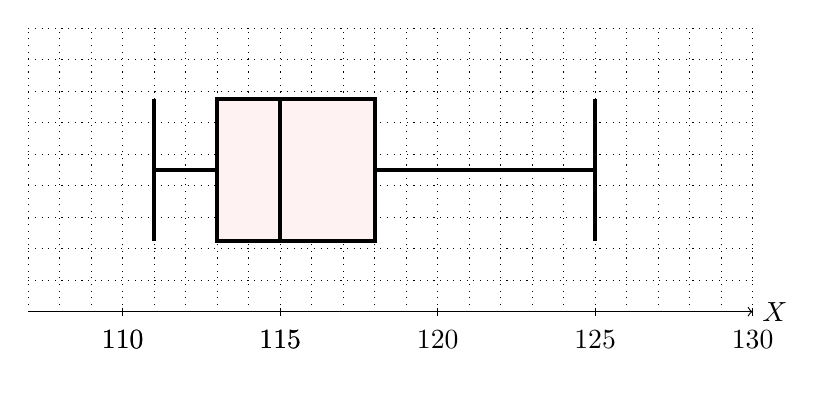
\begin{tikzpicture}[x=0.4cm,y=0.9cm]
         \draw[step=0.4cm,,dotted,color=black] (107,0) grid (130,4);
		\draw[->] (107,0) -- (130,0) node[right] {$X$} ;
		\foreach \X in {110,115,110,115,120,125,130} {
			\draw (\X,0.05cm) -- (\X,-0.05cm) node[below] {$\X\strut$};}
		\draw[ultra thick][fill=red!5] (113,1) rectangle (118,3);
  	\draw[ultra thick] (115,1) -- (115,3);

		\draw[ultra thick] (111,1) -- (111,3);
		\draw[ultra thick] (111,2) -- (113,2);
		\draw[ultra thick] (118,2) -- (125,2);
		%\draw[ultra thick] (4,1) -- (4,3);
		\draw[ultra thick] (125,1) -- (125,3);
			\end{tikzpicture}\\
	\end{center}

\begin{solution}
L'élément manquant est le \textbf{point aberrant} (\textit{outlier}) à $x=128$.

Calcul: $Q_1=113$, $Q_3=118$, $\text{IQR}=Q_3-Q_1=5$. La barrière supérieure est $Q_3+1{,}5\times\text{IQR}=118+7{,}5=125{,}5$. Puisque $128 > 125{,}5$, la valeur 128 est une observation aberrante et devrait être affichée comme un point isolé à $x=128$. La moustache de droite s'arrête correctement à 125 (la plus grande valeur $\leq 125{,}5$).
\end{solution}
 
\part Nous apprenons que la plus grande observation (128) est erronée. Nous ne connaissons pas sa valeur, mais nous savons que celle-ci est plus grande que 150. Nous notons cette valeur XXX et nous savons que XXX~$>$~150. Le nouveau jeu de données est donc:

\begin{center}
\begin{tabular}{  c c c c c c c c }
111  &111  &111  &112  &113  &113  &113 \\
113 &115  &115  &115  &115 &115 & 116 \\
116 & 118 & 118 & 119 & 125 &127 & XXX\\
\end{tabular}
\end{center}

À partir de ce nouveau jeu de données, répondez aux questions suivantes. Nous nommons «jeu de données original» celui qui contient l'observation 128 et «nouveau jeu de données» celui qui contient l'observation XXX.

Déterminez si les énoncés suivants sont vrais ou faux. 

\textbf{\textit{Une bonne réponse vaut 2 points, une mauvaise réponse vaut -1 point et une réponse vide vaut 0 point, pour un total minimum de 0 point.}}

\begin{subparts}
\subpart La médiane échantillonnale du nouveau jeu de données est supérieure à celle du jeu de données original.

    \begin{oneparcheckboxes}
        \choice Vrai
        \correctchoice Faux
    \end{oneparcheckboxes}
    

\subpart La moyenne échantillonnale du nouveau jeu de données est supérieure à celle du jeu de données original.

    \begin{oneparcheckboxes}
        \correctchoice Vrai
        \choice Faux
    \end{oneparcheckboxes}
    

\subpart La variance échantillonnale du nouveau jeu de données est supérieure à celle du jeu de données original.

    \begin{oneparcheckboxes}
        \correctchoice Vrai
        \choice Faux
    \end{oneparcheckboxes}
    

\end{subparts}

\begin{solution}
\begin{subparts}
\subpart Faux. La médiane est à la position 11. Les 11 premières valeurs (111, 111, 111, 112, 113, 113, 113, 113, 115, 115, 115) n'ont pas changé, donc la médiane reste $\tilde{x}=115$.

\subpart Vrai. La valeur XXX $> 150$ remplace 128 (et 127 remplace 125 à la position 20). Puisque XXX $> 128$ et $127 > 125$, la somme augmente et donc $\overline{x}$ augmente.

\subpart Vrai. La valeur XXX $> 150$ est beaucoup plus éloignée de la moyenne que ne l'était 128, ce qui augmente la dispersion et donc la variance échantillonnale.
\end{subparts}
\end{solution}

\end{parts}
\end{A23}

\begin{A24}
\question  (A24)
Soit les 21 valeurs suivantes:

\begin{center}
\begin{tabular}{  c c c c c c c c }
111  &112  &112  &112  &113  &113  &113 \\
113 &115  &115  &115  &115 &115 & 116 \\
118 & 118 & 118 & 119 & 124 &124 & 125\\
\end{tabular}
\end{center}

Le diagramme en boîte ci-dessous a été tracé à partir de ces résultats.

\begin{center}
		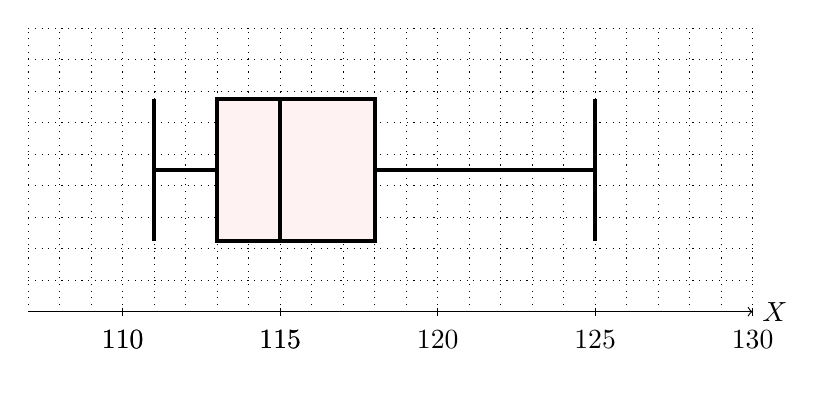
\begin{tikzpicture}[x=0.4cm,y=0.9cm]
         \draw[step=0.4cm,,dotted,color=black] (107,0) grid (130,4);
		\draw[->] (107,0) -- (130,0) node[right] {$X$} ;
		\foreach \X in {110,115,110,115,120,125,130} {
			\draw (\X,0.05cm) -- (\X,-0.05cm) node[below] {$\X\strut$};}
		\draw[ultra thick][fill=red!5] (113,1) rectangle (118,3);
  	\draw[ultra thick] (115,1) -- (115,3);

		\draw[ultra thick] (111,1) -- (111,3);
		\draw[ultra thick] (111,2) -- (113,2);
		\draw[ultra thick] (118,2) -- (125,2);
		%\draw[ultra thick] (4,1) -- (4,3);
		\draw[ultra thick] (125,1) -- (125,3);

			\end{tikzpicture}\\
	\end{center}

Lequel des énoncés suivants est vrai?

  \begin{checkboxes}
\choice La médiane n'est pas au bon endroit.  %  X1
\choice La moyenne échantillonnale n'est pas au bon endroit. % X_2 | X1
\choice Il devrait y avoir deux points: un à 105,5 et un à 125,5.
\choice La moustache de gauche devrait être à  105,5. 
\choice La moustache de droite devrait être à 125,5.
\choice Il y a plus qu'une erreur.
\correctchoice Il n'y a aucune erreur.
\end{checkboxes}

\begin{solution}
Les données triées: 111, 112, 112, 112, 113, 113, 113, 113, 115, 115, 115, 115, 115, 116, 118, 118, 118, 119, 124, 124, 125. Avec $n=21$: $Q_1=x_{(6)}=113$, $\tilde{x}=x_{(11)}=115$, $Q_3=x_{(16)}=118$, $\text{IQR}=5$.

Barrières: inférieure $= 113-7{,}5=105{,}5$, supérieure $= 118+7{,}5=125{,}5$. Toutes les observations sont entre $105{,}5$ et $125{,}5$, donc il n'y a pas de valeurs aberrantes. La boîte va de 113 à 118, la médiane est à 115, les moustaches vont de 111 à 125. Le diagramme est correct: il n'y a aucune erreur.
\end{solution}
\end{A24}

\begin{A25}
\question (A25) Soit l'histogramme suivant:

\begin{center}
    
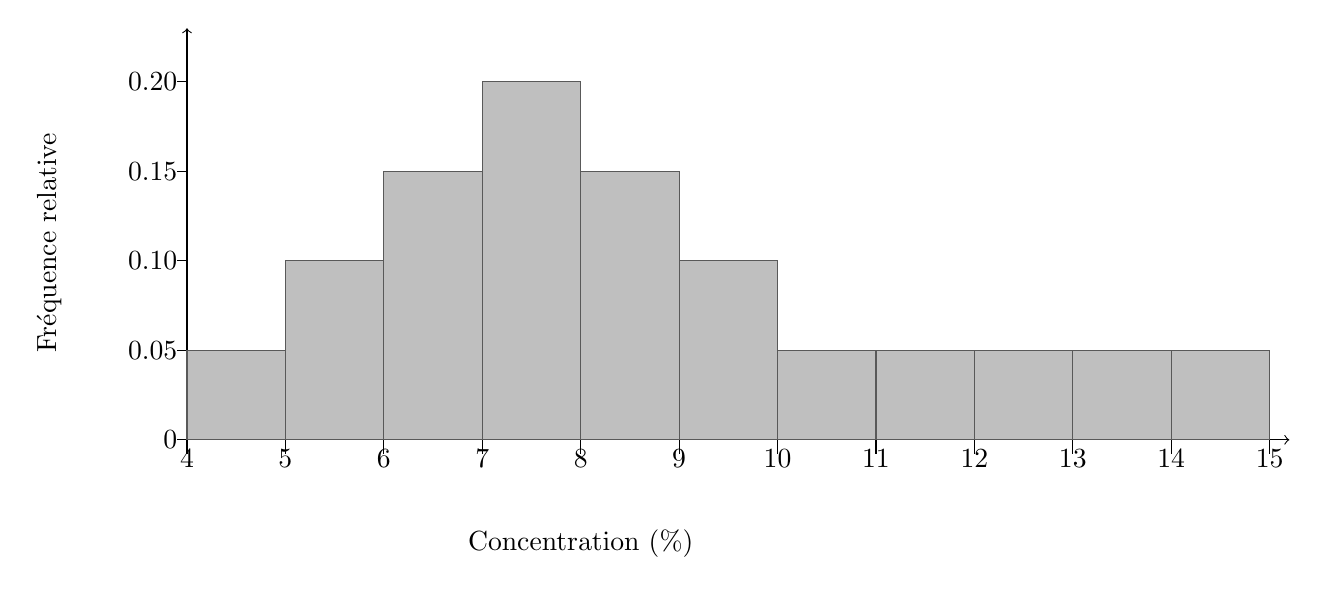
\begin{tikzpicture}[x=1.25cm, y=22.727cm] % 10 cm de large (8 unités) et 5 cm de haut (0.22 unités)
  % Axes
  \draw[->] (4,0) -- (15.2,0);
  \draw[->] (4,0) -- (4,0.23);

  % Graduations en x
  \foreach \x in {4,...,15} {
    \draw (\x,0) -- (\x,-0.008);
    \node[below] at (\x,0) {\x};
  }

  % Graduations en y
  \foreach \y/\lab in {0/0,0.05/0.05,0.10/0.10,0.15/0.15,0.20/0.20}{
    \draw (4,\y) -- (3.9,\y);
    \node[left] at (4,\y) {\lab};
  }

  % Titres d'axes
  \node[below] at (8,-0.045) {Concentration (\%)};
  \node[rotate=90] at (2.6,0.11) {Fréquence relative};

  % Barres : classes [4,5[, [5,6[, ..., [11,12[
  \foreach \x/\h in {4/0.05,5/0.1,6/0.15,7/0.20,8/0.15,9/0.1,10/0.05,11/0.05,12/0.05,13/0.05,14/0.05} {
    \fill[gray!50] (\x,0) rectangle (\x+1,\h);
    \draw[gray!70!black] (\x,0) rectangle (\x+1,\h);
  }
\end{tikzpicture}
\end{center}

Déterminez si les énoncés suivants sont vrais ou faux. 

\textbf{\textit{Une bonne réponse vaut 2 points, une mauvaise réponse vaut -1 point et une réponse vide vaut 0 point, pour un total minimum de 0 point.}}

\begin{parts}
    \part Il est impossible de donner la taille de l'échantillon qui a servi à tracer cet histogramme avec l'information donnée.

    \begin{oneparcheckboxes}
        \correctchoice Vrai
        \choice Faux
    \end{oneparcheckboxes}

\part Cet histogramme est typique de données provenant d'une distribution où la moyenne est supérieure à la médiane.

    \begin{oneparcheckboxes}
        \correctchoice Vrai
        \choice Faux
    \end{oneparcheckboxes}

\part L'écart interquartile vaut au moins 5,5.

    \begin{oneparcheckboxes}
        \choice Vrai
        \correctchoice Faux
    \end{oneparcheckboxes}

    

\part La médiane échantillonnale est entre 7\% et 9\%, inclusivement.

    \begin{oneparcheckboxes}
        \correctchoice Vrai
        \choice Faux
    \end{oneparcheckboxes}

\part L'écart-type échantillonnal est de 11\%.

    \begin{oneparcheckboxes}
        \choice Vrai
        \correctchoice Faux
    \end{oneparcheckboxes}
    
    \end{parts}

\begin{solution}
\begin{parts}
\part Vrai. L'histogramme montre les fréquences relatives (densité). On connaît les proportions dans chaque classe mais pas la taille de l'échantillon $n$.

\part Vrai. L'histogramme est asymétrique à droite (queue plus longue vers la droite), ce qui est typique d'une distribution où la moyenne est supérieure à la médiane.

\part Faux. En utilisant les fréquences relatives cumulées: $F(6)=0{,}15$, $F(7)=0{,}30$, $F(8)=0{,}50$, $F(9)=0{,}65$, $F(10)=0{,}75$. Ainsi, $Q_1 \approx 6{,}67$ (dans $[6,7)$) et $Q_3 = 10$ (fin de $[9,10)$). L'IQR $\approx 3{,}33 < 5{,}5$.

\part Vrai. La médiane correspond au 50$^e$ percentile. $F(7)=0{,}30$ et $F(8)=0{,}50$, donc la médiane est $\tilde{x}=8$, qui est entre 7\% et 9\%.

\part Faux. Il est impossible de calculer l'écart-type exact à partir de l'histogramme sans connaître les valeurs individuelles. De plus, les données s'étendent approximativement de 4 à 15, donc un écart-type de 11\% est irréaliste.
\end{parts}
\end{solution}
\end{A25}

\begin{H26}
\question
(H26)
Dans un laboratoire de microtechnique, Benjamin et Guillaume ont étudié le temps de réaction (en millisecondes) d'un certain type de détecteur de mouvements. Les 21 valeurs suivantes sont des temps de réaction collectés au cours d'une journée:

\begin{center}
\begin{tabular}{  c c c c c c c c }
111  &111  &111  &112  &113  &113  &113 \\
113 &115  &115  &115  &115 &115 & 116 \\
116 & 118 & 118 & 119 & 125 &125 & 128\\
\end{tabular}
\end{center}

Le diagramme en boîte ci-dessous a été tracé à partir de ces résultats. Il manque toutefois quelque chose à ce diagramme (il ne s'agit pas d'un titre ou de noms d'axes).


Ajoutez \textbf{sur le diagramme} l'élément manquant et dites ce que vous avez fait sous le diagramme. Un ajout sur le diagramme sans justification n'aura aucun point.
\begin{center}
		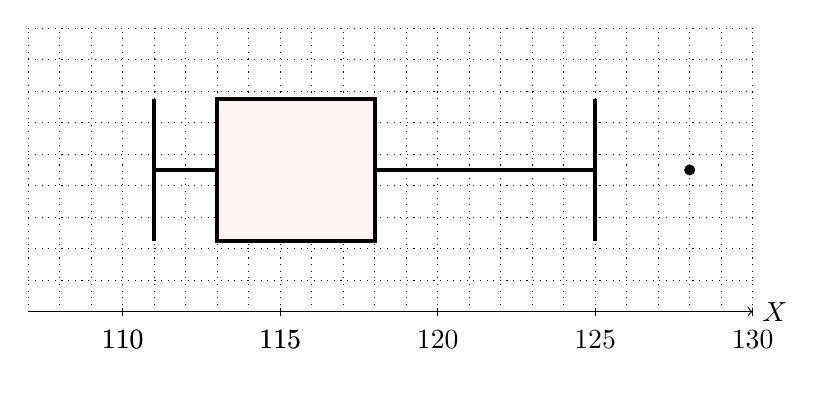
\begin{tikzpicture}[x=0.4cm,y=0.9cm]
         \draw[step=0.4cm,,dotted,color=black] (107,0) grid (130,4);
		\draw[->] (107,0) -- (130,0) node[right] {$X$} ;
		\foreach \X in {110,115,110,115,120,125,130} {
			\draw (\X,0.05cm) -- (\X,-0.05cm) node[below] {$\X\strut$};}
		\draw[ultra thick][fill=red!5] (113,1) rectangle (118,3);


		\draw[ultra thick] (111,1) -- (111,3);
		\draw[ultra thick] (111,2) -- (113,2);
		\draw[ultra thick] (118,2) -- (125,2);
		%\draw[ultra thick] (4,1) -- (4,3);
		\draw[ultra thick] (125,1) -- (125,3);
        \node[circle, fill=black, inner sep=0pt, minimum size=4pt] at (128,2) {};
			\end{tikzpicture}\\
	\end{center}

\begin{solution}
L'élément manquant est la ligne de la \textbf{médiane}. Les données triées sont: 111, 111, 111, 112, 113, 113, 113, 113, 115, 115, 115, 115, 115, 116, 116, 118, 118, 119, 125, 125, 128. Avec $n=21$, la médiane est à la position 11, soit $\tilde{x}=115$.

De plus, $Q_1 = x_{(6)} = 113$, $Q_3 = x_{(16)} = 118$, $\text{IQR} = 5$. La barrière supérieure est $Q_3 + 1{,}5 \times \text{IQR} = 118 + 7{,}5 = 125{,}5$. Puisque $128 > 125{,}5$, la valeur 128 est une observation aberrante (correctement affichée comme un point). La barrière inférieure est $Q_1 - 1{,}5 \times \text{IQR} = 113 - 7{,}5 = 105{,}5$. Aucune observation n'est inférieure à $105{,}5$.

Il faut ajouter une ligne verticale à $x=115$ à l'intérieur de la boîte pour représenter la médiane.
\end{solution}
\end{H26}


\section*{Module 6 - Échantillons aléatoires, lois échantillonnales et estimation ponctuelle}
\begin{H23}
\question 
(H23, A23)
Soit $X_1, \hdots, X_9$ un échantillon aléatoire d'une variable $X\sim\mathcal{N}(12, 4)$. Nous avons que $X_1, \dots, X_9$ sont indépendantes. 

\begin{parts}
    \part Calculez la probablité que la moyenne échantillonnale soit supérieure à la vraie moyenne $\mu = 12$ par plus de 0,62 écarts-types échantillonnaux. 

\begin{solution}
On cherche $P(\overline{X} > \mu + 0{,}62\,S) = P(\overline{X} - 12 > 0{,}62\,S)$.

En divisant par $S/\sqrt{n}=S/3$:
$$P\!\left(\frac{\overline{X}-12}{S/3} > \frac{0{,}62\,S}{S/3}\right) = P\!\left(T > 0{,}62 \times 3\right) = P(T > 1{,}86),$$
où $T = \dfrac{\overline{X}-\mu}{S/\sqrt{n}} \sim t_{n-1} = t_8$.

De la table de Student: $t_{8;\,0{,}05} = 1{,}860$, donc $P(t_8 > 1{,}86) = 0{,}05$.
\end{solution}

    \part Calculez la probabilité que la variance échantillonnale soit inférieure à 1,09.

\begin{solution}
On sait que $\dfrac{(n-1)S^2}{\sigma^2} \sim \chi^2_{n-1}$, soit $\dfrac{8S^2}{4} = 2S^2 \sim \chi^2_8$.

$$P(S^2 < 1{,}09) = P(2S^2 < 2{,}18) = P(\chi^2_8 < 2{,}18).$$

De la table du khi-deux: $\chi^2_{8;\,0{,}975} = 2{,}180$ (quantile tel que l'aire à gauche vaut $0{,}025$), donc $P(\chi^2_8 < 2{,}18) = 0{,}025$.
\end{solution}

\end{parts}
\end{H23}

\begin{H23}
\question (H23) Soit $T$, une variable aléatoire Student à 5 degrés de libertés. Nous notons $\mu_T$~et~$\sigma^2_T$, l'espérance et la variance de $T$, respectivement. Laquelle des affirmations suivantes est vraie? %module 5

\begin{checkboxes}
\choice $\displaystyle Z=\frac{T-\mu_T}{\sigma_T}\sim \mathcal{N}(0, 1)$
\choice Nous savons que $\mu_T=5$ et $\sigma^2_T=10$
\CorrectChoice La fonction de densité de $T$ est symétrique
\choice La fonction de répartition de $T$ est symétrique
\end{checkboxes}
\end{H23}

\begin{H23}
\question (H23)Soit $K$, $G$ et $M$ des variables aléatoires indépendantes qui suivent respectivement une khi-carré à 4 degrés de liberté, une Student à 3 degrés de liberté et une Fisher à 3 et 4 degrés de liberté. 

Que vaut $P(K>1,06~\cap~G~>~0,277~\cap~M~<~16,69)$?

\begin{oneparcheckboxes}
		\correctchoice 0,3564
		\choice 0,5346
		\choice 0,0036
		\choice 0,0054
		\choice 0,0396
\end{oneparcheckboxes}
\end{H23}

\begin{A23}
\question (A23) Laquelle des affirmations suivantes est toujours vraie au sujet de $\overline{X}=\displaystyle \frac{1}{n}\sum_{i=1}^n X_i$, où les $X_i$ sont indépendants et identiquement distribués de loi quelconque d'espérance $\mu_X$ et de variance $\sigma^2_X$? %module 5

\begin{checkboxes}
\choice $\displaystyle Z=\frac{\overline{X}-\mu_X}{\sigma_X / \sqrt{n}}\sim \mathcal{N}(0, 1)$

\choice $\mathbb{E}\left[\overline{X}\right]=\mu_X$ seulement si $n>30$

\correctchoice $\mathbb{E}\left[\overline{X}\right]=\mu_X$ peu importe la loi des $X_i$

\choice $\displaystyle\mathbb{E}\left[\overline{X}\right]=\mu_X$  seulement si les $X_i$ sont de loi normale

\choice $\text{Var}\left[\overline{X}\right]=\sigma^2_X$
\end{checkboxes}
\end{A23}

\begin{H24}
\question (H24) Soit $K$, $S$ et $F$ des variables aléatoires indépendantes qui suivent respectivement une khi-carré à 4 degrés de liberté, une Student à 35 degrés de liberté et une Fisher à 3 et 4 degrés de liberté. 

Cochez tous les énoncés qui sont \textbf{faux}?

\begin{checkboxes}
		\correctchoice $P(S>35)=0,50$
		\choice $P(K<9,49)=0,95$
		\choice $P(F>6,59)=0,05$
		\choice $P(S>a \cap K> b \cap F >c)= P(S>a)\times P(K>b)\times P(F>c)$
\end{checkboxes}
\end{H24}

    \begin{A24}
    \question (A24) Soit deux échantillons aléatoires indépendants provenant de populations normales, tels que:
\begin{align*}
    X_1,\hdots,X_{16}&\sim\mathcal{N}(7, 4),\\
    Y_1,\hdots,Y_{100}&\sim\mathcal{N}(8, 9).
\end{align*}

\begin{parts}
\part Quelle est la loi de $A=X_1+X_2-X_3$?
    \begin{checkboxes}
        \choice $A\sim\mathcal{N}(7; 8)$
        \choice $A\sim\mathcal{N}(7; 12)$
        \choice $A\sim\mathcal{N}(14; 8)$
        \choice $A\sim\mathcal{N}(14; 12)$
        \choice $A\sim\mathcal{N}(21; 8)$
        \choice $A\sim\mathcal{N}(21; 12)$
        \choice Aucune de ces réponses
    \end{checkboxes}
    

    \part Quelle est la loi de $B=\displaystyle\frac{1}{100}\sum_{i=1}^{100}Y_i$?
        \begin{checkboxes}
        \choice $B\sim\mathcal{N}(0,08; 9)$
        \choice $B\sim\mathcal{N}(0,08; 0,81)$
        \choice $B\sim\mathcal{N}(0,08; 0,09)$
        \choice $B\sim\mathcal{N}(8; 9)$
        \choice $B\sim\mathcal{N}(8; 0,81)$
        \choice $B\sim\mathcal{N}(8; 0,09)$
        \choice Aucune de ces réponses
    \end{checkboxes}

    
    \part Quelle est la loi de $C=X_1$?
        \begin{checkboxes}
        \choice $C\sim\mathcal{N}(0,4375; 4)$
        \choice $C\sim\mathcal{N}(0,4375; 0,25)$
        \choice $C\sim\mathcal{N}(0,4375; 1)$
        \choice $C\sim\mathcal{N}(7; 4)$
        \choice $C\sim\mathcal{N}(7; 0,25)$
        \choice $C\sim\mathcal{N}(7
        ; 1)$
        \choice Aucune de ces réponses
    \end{checkboxes}
   \part Quelle est l'espérance de $D=\displaystyle\frac{\overline{Y}-8}{S_Y/10}$, où $S_Y$ est l'écart-type échantillonnal de $Y$?
        \begin{checkboxes}
        \choice $E(D)=8$
        \choice $E(D)=100$
        \choice $E(D)=99$
        \choice $E(D)=0$
        \choice $E(D)=15$
        \choice $E(D)=800$
        \choice Aucune de ces réponses
    \end{checkboxes}
\end{parts}
    \end{A24}

\begin{A24}
\question (A24)
Déterminez si les énoncés suivants sont vrais ou faux. 

\textbf{\textit{Une bonne réponse vaut 2 points, une mauvaise réponse vaut -1 point et une réponse vide vaut 0 point, pour un total minimum de 0 point.}}

\begin{parts}
    \part Si $X_1,\hdots,X_{100}$ constituent un échantillon aléatoire simple issu d'une loi normale d'espérance $\mu=16$ et de variance $\sigma^2=100$, alors la moyenne échantillonnale de ces 100 valeurs suit approximativement une loi normale centrée-réduite. 

    \begin{oneparcheckboxes}
        \choice Vrai
        \correctchoice Faux
    \end{oneparcheckboxes}

  
    
    \part Si $X_1,\hdots,X_{17}$ constituent un échantillon aléatoire simple issu d'une loi $\mathcal{N}(5; 4)$, alors la variable $4S^2$ a une espérance de 16 et une variance de 32. 

    \begin{oneparcheckboxes}
        \choice Vrai
        \correctchoice Faux
    \end{oneparcheckboxes}
    
        

    \part Si $W$ suit une $\chi^2_4$ (khi-carré avec $4$ degrés de liberté), alors $P(W>4)=P(W<4)$. 

    \begin{oneparcheckboxes}
        \choice Vrai
        \correctchoice Faux
    \end{oneparcheckboxes}
    
 
        
    \item Le poids des tomates d'un certain agriculteur suit une loi normale de moyenne $300\text{ grammes}$ et de variance $100\text{ grammes}^2$. On prend des mesures sur 25 tomates choisies aléatoirement et on obtient une moyenne échantillonnale de $309,12\text{ grammes}$ et une variance échantillonnale de $118,3\text{ grammes}^2$. Dans cette situation, les nombres $309,12$ et $118,3$ sont des paramètres et les nombres $300$ et $100$ sont des statistiques.
    
    \begin{oneparcheckboxes}
        \choice Vrai
        \correctchoice Faux
    \end{oneparcheckboxes}
   
        

    \part Soit deux échantillons aléatoires indépendants de taille $n=26$ et $m=26$ qui proviennent de lois normales $\mathcal{N}(\mu_X, \sigma_X^2)$ et $\mathcal{N}(\mu_Y, \sigma_Y^2)$. Les moyennes échantillonnales sont respectivement $\overline{X}$ et $\overline{Y}$, alors que les variances échantillonnales sont respectivement $S^2_X$ et $S^2_Y$. La statistique ${\displaystyle S^2_X}/ {\displaystyle S^2_Y}$ suit une $F_{25,25}$. 

    \begin{oneparcheckboxes}
        \choice Vrai
        \correctchoice Faux
    \end{oneparcheckboxes}
    

    \end{parts}
\end{A24}

    \begin{A24}
    \question (A24)  
Soit $X_1,\hdots,X_9$ des réalisations indépendantes d'une variable $X\sim\mathcal{N}(12, 24)$ et $Y_1,\hdots,Y_{18}$ des réalisations indépendantes d'une variable $Y\sim\mathcal{N}(21, 24)$. 
Notez $S_X^2$ et $S_Y^2$, les variances des deux échantillons.

Quelle est la probabilité que $S_X^2$ soit deux fois plus grande que $S_Y^2$?
    \end{A24}

\begin{A25}
\question\label{AOVblocs1} (A25)

Un échantillon aléatoire $X_1,\dots,X_n$ est obtenu à partir d'une loi dont la fonction
de densité dépend d'un paramètre inconnu $\theta$. Une prise de décision en ingénierie
repose sur la valeur de la probabilité $P(X_i>0,5)$. Or pour ce modèle, 
cette probabilité est égale à $e^{-0,5\theta}$.

On vous propose deux estimateurs $\hat{P}_1$ et $\hat{P}_2$ qui ont les propriétés suivantes :
\begin{align*}
    E(\hat{P}_1)&= e^{-0,5\theta},&  V(\hat{P}_1) =& \frac{e^{-0,5\theta}\left(1-e^{-0,5\theta}\right)}{n}, \\
    E(\hat{P}_2) &= \theta,&  V(\hat{P}_2) =&\frac{\theta^2}{n} .
\end{align*}

Quels sont les \textbf{trois} énoncés qui sont \textbf{vrais} parmi les six énoncés ci-dessous ?

\begin{checkboxes}
    \correctchoice $\hat{P}_1$ est un estimateur sans biais de $e^{-0,5\theta}$.
 
\choice $\hat{P}_2$ est un estimateur sans biais de $e^{-0,5\theta}$.

\choice L'erreur quadratique moyenne de $\hat{P}_1$ en tant qu'estimateur de $e^{-0,5\theta}$ est égale à 
$$e^{-\theta}+\frac{e^{-0,5\theta}\left(1-e^{-0,5\theta}\right)}{n}.$$
    \correctchoice L'erreur quadratique moyenne de $\hat{P}_2$ en tant qu'estimateur de $e^{-0,5\theta}$
est égale à 
$$\left(\theta-e^{-0,5\theta}\right)^2+\frac{\theta^2}{n}.$$
\correctchoice L'erreur quadratique moyenne de $\hat{P}_1$ en tant qu'estimateur de $e^{-0,5\theta}$ est égale à 
$V(\hat{P}_1)$.

\choice L'erreur quadratique moyenne de $\hat{P}_2$ en tant qu'estimateur de $e^{-0,5\theta}$ est égale à 
$V(\hat{P}_2)$.
\end{checkboxes}
\end{A25}

\begin{A25}
\question (A25) La quantité de pluie (en mm) tombée dans un bassin versant
dans un mois suit une loi ayant comme fonction de répartition
$$F(x)=\left\{\begin{array}{ll}
0, & x<0\\
1-e^{-x/\theta}, & x\ge 0,
\end{array}\right.$$
où $\theta>0$ est un paramètre de valeur inconnue. On peut montrer que $E(X)=\theta$ et $V(X)=\theta^2$.

La compagnie qui gère un barrage à la sortie de ce bassin versant a besoin de savoir l'espérance et la variance de la quantité de pluie tombée
dans un mois afin d'optimiser la gestion du barrage. L'ingénieure de la compagnie a à sa disposition un échantillon aléatoire $X_1,\dots,X_{20}$
provenant de cette loi, dont elle souhaite se servir pour estimer les quantités désirées. Soit $\displaystyle \overline{X}=\frac{1}{20}\sum_{i=1}^{20}X_i$.

    \begin{parts}
    \part Calculez l'espérance de $\overline{X}$. Est-ce que $\overline{X}$ est un estimateur sans biais de $\theta$ ? 

\begin{solution}
$E(\overline{X}) = E\!\left(\dfrac{1}{20}\displaystyle\sum_{i=1}^{20}X_i\right) = \dfrac{1}{20}\times 20\,\theta = \theta$.

Puisque $E(\overline{X})=\theta$, $\overline{X}$ est un estimateur \textbf{sans biais} de $\theta$.
\end{solution}

    \part  Calculez l'espérance de $\overline{X}^2$. Est-ce que $\overline{X}^2$ est un estimateur sans biais de $\theta^2$ ?
    
    [Aide :\ Souvenez-vous que pour toute variable aléatoire $Y$,\ \ $V(Y)=E(Y^2)-\{E(Y)\}^2$.\ \ \ \ ]

\begin{solution}
On utilise $E(Y^2) = V(Y) + [E(Y)]^2$ avec $Y=\overline{X}$:
$$V(\overline{X}) = \frac{V(X_1)}{20} = \frac{\theta^2}{20}.$$
$$E(\overline{X}^2) = V(\overline{X}) + [E(\overline{X})]^2 = \frac{\theta^2}{20} + \theta^2 = \frac{21\theta^2}{20}.$$

Puisque $E(\overline{X}^2) = \dfrac{21\theta^2}{20} \neq \theta^2$, $\overline{X}^2$ n'est \textbf{pas} un estimateur sans biais de $\theta^2$.

Le biais est $E(\overline{X}^2)-\theta^2 = \dfrac{21\theta^2}{20}-\theta^2 = \dfrac{\theta^2}{20}$.
\end{solution}
 
    \end{parts}
\end{A25}

    \begin{A25}
    \question (A25) Soit $X_1,\hdots,X_{25}$, des réalisations indépendantes d'une variable aléatoire normale d'espérance $\mu=176,45$ et d'écart-type $\sigma=\sqrt{48}$.

    \begin{parts}
        \part Quelle est la probabilité que la variance échantillonnale soit supérieure à 46,68?

\begin{solution}
On sait que $\dfrac{(n-1)S^2}{\sigma^2}\sim\chi^2_{n-1}$, soit $\dfrac{24S^2}{48}=\dfrac{S^2}{2}\sim\chi^2_{24}$.

$$P(S^2>46{,}68)=P\!\left(\frac{S^2}{2}>\frac{46{,}68}{2}\right)=P(\chi^2_{24}>23{,}34).$$

De la table du khi-deux: $\chi^2_{24;\,0{,}50}\approx 23{,}337$, donc $P(\chi^2_{24}>23{,}34)\approx 0{,}50$.
\end{solution}

        \part Quelle est la probabilité que la moyenne échantillonale soit supérieure à $\mu+0,749 ~ S$, où $S$ est l'écart-type échantillonnal ?

\begin{solution}
On cherche $P(\overline{X}>\mu+0{,}749\,S)$. En divisant par $S/\sqrt{n}=S/5$:
$$P\!\left(\frac{\overline{X}-\mu}{S/5}>0{,}749\times 5\right)=P(T>3{,}745),$$
où $T=\dfrac{\overline{X}-\mu}{S/\sqrt{n}}\sim t_{n-1}=t_{24}$.

De la table de Student: $t_{24;\,0{,}0005}=3{,}745$, donc $P(t_{24}>3{,}745)=0{,}0005$.
\end{solution}
 
    \end{parts}
    \end{A25}

\begin{H26}
\question (H26) 
Soit $X_1,\hdots,X_5$ un échantillon de taille $n=5$ provenant d'une variable aléatoire de fonction de répartition $F_X$, d'espérance $\mu$ et de variance $\sigma^2$.

    Pour estimer $\mu$, nous voulons comparer la performance de deux estimateurs:

    \begin{align*}
        \hat{\mu}_1=\overline{X}, & & \hat{\mu}_2=0,1X_1+0,2X_2+0,2X_3+0,2X_4+0,1X_5.
    \end{align*}

    \begin{parts}
        \part Lequel des deux estimateurs a la plus faible variance?

\begin{solution}
$V(\hat{\mu}_1) = V(\overline{X}) = \dfrac{\sigma^2}{5} = 0{,}2\sigma^2$.

$V(\hat{\mu}_2) = (0{,}1^2+0{,}2^2+0{,}2^2+0{,}2^2+0{,}1^2)\sigma^2 = (0{,}01+0{,}04+0{,}04+0{,}04+0{,}01)\sigma^2 = 0{,}14\sigma^2$.

Puisque $0{,}14\sigma^2 < 0{,}2\sigma^2$, c'est $\hat{\mu}_2$ qui a la plus faible variance.
\end{solution}
    
        \part On sait que $biais(\hat{\mu}_2,\mu)=-0,2\mu$. En supposant que $\sigma^2=1$, pour quelles valeurs de $\mu$ a-t-on que l'estimateur $\hat{\mu}_2$ est meilleur que $\hat{\mu}_1$ au niveau du MSE?

\begin{solution}
$\hat{\mu}_1=\overline{X}$ est sans biais, donc $\text{MSE}(\hat{\mu}_1,\mu)=V(\hat{\mu}_1)=\dfrac{\sigma^2}{5}=\dfrac{1}{5}=0{,}2$.

$\text{MSE}(\hat{\mu}_2,\mu)=V(\hat{\mu}_2)+[\text{biais}(\hat{\mu}_2,\mu)]^2=0{,}14\sigma^2+(-0{,}2\mu)^2=0{,}14+0{,}04\mu^2$.

$\hat{\mu}_2$ est meilleur lorsque $\text{MSE}(\hat{\mu}_2,\mu)<\text{MSE}(\hat{\mu}_1,\mu)$:
$$0{,}14+0{,}04\mu^2 < 0{,}2 \implies 0{,}04\mu^2<0{,}06 \implies \mu^2<1{,}5 \implies |\mu|<\sqrt{1{,}5}=\frac{\sqrt{6}}{2}\approx 1{,}225.$$
\end{solution}

        \end{parts}
\end{H26}
\section*{Module 7 - Intervalles de confiance}
\begin{H24}
\question (H24) Nous nous intéressons aux prix des loyers des étudiants de l'Université Laval. 
Avec un échantillon aléatoire de $n=241$ étudiants, nous obtenons l'intervalle de confiance à 95\%  pour $\mu$ suivant: $[550;1630]$. 
Cochez tous les énoncés qui sont vrais parmi les suivants. \textit{\textbf{Une réponse cochée alors qu'elle ne devrait pas l'être entraîne une pénalité de 1 point. Le minimum possible pour cette question est 0 point.}}
 
\begin{checkboxes}
\choice Il y a 95\% des étudiants qui ont un loyer entre 550 \$ et 1630 \$
\choice Si on choisissait un échantillon de 100 étudiants pour construire un nouvel intervalle de confiance à 95\% sur la moyenne, celui-ci aurait une plus faible probabilité de contenir la vraie valeur de $\mu$ que celui obtenu à partir de 241 étudiants.
\choice Si on choisissait un autre échantillon de 241 étudiants pour construire un intervalle de confiance à 95\% sur la moyenne, l'intervalle obtenu aurait nécessairement la même longueur que celui-ci.
\correctchoice Si on choisissait plusieurs échantillons de 241 étudiants dans cette population, et qu'on construisait avec chacun d'eux l'intervalle de confiance à 95\% pour $\mu$, alors environ 95\% de ces intervalles contiendraient la vraie valeur moyenne des loyers des étudiants de l'Université Laval. 
\correctchoice Si on suppose que le prix des loyers ne suit pas une loi normale, l'intervalle de confiance est toujours valide, car $n\geq 30$, mais son niveau est approximatif.
\end{checkboxes}
\begin{solution}
\begin{itemize}
    \item \textbf{Choix 1 (Faux):} L'IC porte sur la moyenne $\mu$, pas sur les observations individuelles. On ne peut pas conclure que 95\% des étudiants ont un loyer dans cet intervalle.
    \item \textbf{Choix 2 (Faux):} Le niveau de confiance reste 95\% quel que soit $n$. Avec un $n$ plus petit, l'IC serait plus large, mais la probabilité de contenir $\mu$ resterait 95\%.
    \item \textbf{Choix 3 (Faux):} La longueur de l'IC dépend de l'écart-type échantillonnal $S$, qui varie d'un échantillon à l'autre. L'intervalle n'aurait donc pas nécessairement la même longueur.
    \item \textbf{Choix 4 (Vrai):} C'est l'interprétation fréquentiste correcte de l'intervalle de confiance.
    \item \textbf{Choix 5 (Vrai):} Par le théorème central limite, si $n \geq 30$, l'approximation normale pour $\bar{X}$ est valide même si $X$ ne suit pas une loi normale. Le niveau est alors approximatif.
\end{itemize}
\end{solution}
\end{H24}

\begin{H24}
\question (H24) Soit $X_1,\hdots, X_{25}$, des variables aléatoires indépendantes de loi normale d'espérance $\mu$ et de variance $\sigma^2$. Voici plusieurs intervalles:
\begin{center}
    
\begin{tabular}{|c|c|c|c|c|}
	\cline{1-2}\cline{4-5}
	&&&&\\[-3mm]
	% Puissance et alpha
	1 &  $\displaystyle \overline {X}\Mypm t_{\sfrac{\alpha}{2};24}\frac{S}{\sqrt{25}}$
	% puissance:  ici, conditionnellement à \mu=\mu_0 plutôt que \mu=\mu_1 
	% bon alpha
	 & \hspace{0.3cm} &
	 6 &  $\displaystyle \overline {X}\Mypm z_{\sfrac{\alpha}{2}}\frac{\sigma^2}{\sqrt{25}}$
	% ici, \overline{X}- moyenne échantillonnale plutôt que \overline{X}- \mu_0 
	\\[4mm]
	\cline{1-2}\cline{4-5}
	&&&&\\[-3mm]
	 2 & $\displaystyle \overline {X}\Mypm t_{\sfrac{\alpha}{2};25}\frac{S}{\sqrt{25}}$
	% ici  divisé par \sigma^2/n plutot que la racine
	&  &
	 7 & $\displaystyle \overline {X}\Mypm t_{\sfrac{\alpha}{2};24}\frac{S}{\sqrt{24}}$ 
	% ici, bonne réponse pour alpha
	\\[4mm]
	\cline{1-2}\cline{4-5}
	&&&&\\[-3mm]
	 3 & $\displaystyle \overline {X}\Mypm t_{\sfrac{\alpha}{2};25}\frac{\sigma}{\sqrt{24}}$
	% ici, conditionnellement à \mu=\mu_0  ET mauvais z_\alpha
	 &  &
	  8 & $\displaystyle \overline {X}\Mypm z_{\sfrac{\alpha}{2}}\frac{S}{\sqrt{25}}$
	 % ici,  mauvais z_\alpha
	 \\[4mm]
	 \cline{1-2}\cline{4-5}
	 &&&&\\[-3mm]
	   4 & $\displaystyle \overline {X}\Mypm t_{\sfrac{\alpha}{2};25}\frac{\sigma}{\sqrt{25}}$
	 % ici avec z_{\alpha/2} plutot que z_\alpha ET divisé par \sigma^2/n plutot que la racine
	 &  &
	  9 & $\displaystyle \left[\frac{24S^2}{\chi_{\sfrac{\alpha}{2};24}^2};\frac{24S^2}{\chi_{1-\sfrac{\alpha}{2};24}^2}\right]$
	 % ici, centrer avec \mu_1 plutot que \mu_0 
	 \\[5mm]
	 \cline{1-2}\cline{4-5}
	 &&&&\\[-3mm]
	  5 & $\displaystyle \overline {X}\Mypm z_{\sfrac{\alpha}{2}}\frac{\sigma}{\sqrt{25}}$
	 % ici avec z_{\alpha/2} plutot que z_\alpha	 
	 &  &
	  10 & $\displaystyle \left[\frac{25S^2}{\chi_{\sfrac{\alpha}{2};25}^2};\frac{25S^2}{\chi_{1-\sfrac{\alpha}{2};25}^2}\right]$
	 % ici, divisé par \sigma^2/n plutot que \sqrt{ \sigma^2/n }
	 \\[5mm]
	 \cline{1-2}\cline{4-5}

	
\end{tabular}

\end{center}

Associez chacune des situations suivantes au numéro de l'intervalle de confiance de niveau $1-\alpha$ qui correspond. Une seule réponse est bonne pour chaque situation.

\begin{parts}
    \part Intervalle de confiance pour $\mu$ lorsque $\sigma^2$ est connue.

  
 \begin{oneparcheckboxes}
     \choice 1
     \choice 2 
     \choice 3 
     \choice 4 
     \CorrectChoice 5 
     \choice 6 
     \choice 7 
     \choice 8 
     \choice 9
     \choice 10
 
 \end{oneparcheckboxes}
 \begin{solution}
 Choix 5. Les $X_i$ sont de loi normale et $\sigma^2$ est connue, donc la quantité pivot est $Z = \frac{\bar{X} - \mu}{\sigma/\sqrt{n}} \sim \mathcal{N}(0,1)$, ce qui donne l'IC $\bar{X} \pm z_{\alpha/2} \frac{\sigma}{\sqrt{25}}$.
 \end{solution}
 
    \part Intervalle de confiance pour $\sigma^2$.
    
  
\begin{oneparcheckboxes}
     \choice 1
     \choice 2 
     \choice 3 
     \choice 4 
     \choice 5 
     \choice 6 
     \choice 7 
     \choice 8 
     \CorrectChoice 9
     \choice 10

 \end{oneparcheckboxes}
 \begin{solution}
 Choix 9. Pour estimer $\sigma^2$ avec des $X_i$ normales, on utilise la quantité pivot $\frac{(n-1)S^2}{\sigma^2} \sim \chi^2_{n-1}$, ce qui donne l'IC $\left[\frac{24S^2}{\chi^2_{\alpha/2;\,24}} \;;\ \frac{24S^2}{\chi^2_{1-\alpha/2;\,24}}\right]$.
 \end{solution}

     \part Intervalle de confiance pour $\mu$ lorsque $\sigma^2$ est inconnue.
    
  
\begin{oneparcheckboxes}
     \CorrectChoice 1
     \choice 2 
     \choice 3 
     \choice 4 
     \choice 5 
     \choice 6 
     \choice 7 
     \choice 8 
     \choice 9
     \choice 10

 \end{oneparcheckboxes}
 \begin{solution}
 Choix 1. Les $X_i$ sont de loi normale et $\sigma^2$ est inconnue, donc on utilise la loi de Student avec $(n-1) = 24$ degrés de liberté: $T = \frac{\bar{X} - \mu}{S/\sqrt{n}} \sim t_{24}$, ce qui donne l'IC $\bar{X} \pm t_{\alpha/2;\,24} \frac{S}{\sqrt{25}}$.
 \end{solution}
 \end{parts}

 \question

(A23)
Un intervalle de confiance au niveau 95\% pour l'espérance $\mu$ est $[10,11 ; 19,11]$. Pour chaque énoncé qui suit, indiquez si l'énoncé est vrai, faux ou si nous n'avons pas assez d'information pour le savoir.

\begin{parts}
    \part Au seuil 5\%, on rejette $H_0: \mu=10$ pour $H_1:\mu \neq 10$.

    \begin{oneparcheckboxes}
        \CorrectChoice Vrai 
        \choice Faux
        \choice Nous n'avons pas assez d'information pour le savoir.
    \end{oneparcheckboxes}
    \begin{solution}
    Vrai. L'IC de niveau 95\% pour $\mu$ est $[10{,}11\;;\;19{,}11]$. Puisque $\mu_0 = 10 \notin [10{,}11\;;\;19{,}11]$, on rejette $H_0: \mu = 10$ au seuil $\alpha = 5\%$.
    \end{solution}

   \part Au seuil 1\%, on rejette $H_0: \mu=10$ pour $H_1:\mu \neq 10$.

   \begin{oneparcheckboxes}
        \choice Vrai 
        \choice Faux
        \CorrectChoice Nous n'avons pas assez d'information pour le savoir.
    \end{oneparcheckboxes}
    \begin{solution}
    Nous n'avons pas assez d'information. L'IC de niveau 95\% exclut $\mu_0 = 10$, donc on rejette au seuil 5\%. Cependant, un IC de niveau 99\% serait plus large et pourrait contenir $\mu_0 = 10$. On ne peut pas conclure au seuil 1\% à partir de l'IC à 95\% seulement.
    \end{solution}
    
   \part Au seuil 10\%, on rejette $H_0: \mu=10$ pour $H_1:\mu \neq 10$.

   \begin{oneparcheckboxes}
        \CorrectChoice Vrai 
        \choice Faux
        \choice Nous n'avons pas assez d'information pour le savoir.
    \end{oneparcheckboxes}
    \begin{solution}
    Vrai. Si on rejette $H_0$ au seuil 5\%, on rejette aussi à tout seuil $\alpha > 5\%$, en particulier au seuil 10\%. En effet, l'IC à 90\% est inclus dans l'IC à 95\%, donc si $\mu_0 = 10$ est à l'extérieur de l'IC à 95\%, il est \textit{a fortiori} à l'extérieur de l'IC à 90\%.
    \end{solution}
    
   \part Au seuil 5\%, on rejette $H_0: \mu=28$ pour $H_1:\mu \neq 28$.

   \begin{oneparcheckboxes}
        \CorrectChoice Vrai 
        \choice Faux
        \choice Nous n'avons pas assez d'information pour le savoir.
    \end{oneparcheckboxes}
    \begin{solution}
    Vrai. Puisque $\mu_0 = 28 \notin [10{,}11\;;\;19{,}11]$, on rejette $H_0: \mu = 28$ au seuil $\alpha = 5\%$.
    \end{solution}
    
%   \part[1] Au seuil 1\%, on rejette $H_0: \mu=8$ pour $H_1:\mu \neq 8$.

%   \begin{oneparcheckboxes}
%        \choice Vrai 
%        \CorrectChoice Faux
%        \choice Nous n'avons pas assez d'information pour le savoir.
%    \end{oneparcheckboxes}

\end{parts}
\end{H24}

\begin{A24}
\question (A24) On a noté la fréquence cardiaque de neuf hommes. 
L'intervalle de confiance à 90\% obtenu pour la fréquence cardiaque moyenne est $[94; 112]$.
On suppose que la loi normale est adéquate pour cette variable aléatoire.

Déterminez si les énoncés suivants sont vrais ou faux. 

\textbf{\textit{Une bonne réponse vaut 1 point, une mauvaise réponse vaut -0,5 point et une réponse vide vaut 0 point, pour un total minimum de 0 point.}}

\begin{parts}
    \part La fréquence cardiaque moyenne des hommes ayant participé à l'étude est de 100 battements par minute.
    
    \begin{oneparcheckboxes}
        \choice Vrai
        \correctchoice Faux
    \end{oneparcheckboxes}
    \begin{solution}
    Faux. La moyenne échantillonnale est le centre de l'intervalle de confiance: $\bar{x} = \frac{94 + 112}{2} = 103$ bpm, et non 100 bpm.
    \end{solution}

    \part Si on recommençait la même expérience avec neuf autres individus de la même population, il y aurait 90\% de chances que la nouvelle moyenne échantillonnale soit comprise entre 94 et 112.
    
    \begin{oneparcheckboxes}
        \choice Vrai
        \correctchoice Faux
    \end{oneparcheckboxes}
    \begin{solution}
    Faux. L'intervalle de confiance est une estimation de $\mu$, pas une prédiction pour une future moyenne échantillonnale $\bar{X}$. Un nouvel échantillon donnerait une nouvelle valeur de $\bar{X}$ et un nouvel IC, possiblement différent de $[94; 112]$.
    \end{solution}

    \part Environ 90\% des hommes de cette population ont une fréquence cardiaque comprise entre 94 et 112.
    
    \begin{oneparcheckboxes}
        \choice Vrai
        \correctchoice Faux
    \end{oneparcheckboxes}
    \begin{solution}
    Faux. L'intervalle de confiance porte sur la moyenne $\mu$ de la population, pas sur les observations individuelles. Ce n'est pas un intervalle de tolérance.
    \end{solution}

    \part Environ 90\% des hommes de cet échantillon ont une fréquence cardiaque comprise entre 94 et 112.
    
    \begin{oneparcheckboxes}
        \choice Vrai
        \correctchoice Faux
    \end{oneparcheckboxes}
    \begin{solution}
    Faux. L'IC est un intervalle pour $\mu$, pas pour les observations individuelles. Il ne permet pas de conclure sur la proportion d'individus ayant une fréquence dans cet intervalle.
    \end{solution}

    \part La probabilité que la moyenne échantillonnale soit comprise entre 94 et 112 est 90\%.
    
    \begin{oneparcheckboxes}
        \choice Vrai
        \correctchoice Faux
    \end{oneparcheckboxes}
    \begin{solution}
    Faux. Pour cet échantillon, $\bar{x} = 103$ est une valeur fixe (réalisée). La moyenne échantillonnale est déjà observée; on ne peut pas lui attribuer une probabilité.
    \end{solution}

    \part La probabilité que la moyenne de la population soit comprise entre 94 et 112 est 90\%.
    
    \begin{oneparcheckboxes}
        \choice Vrai
        \correctchoice Faux
    \end{oneparcheckboxes}
    \begin{solution}
    Faux. Dans le paradigme fréquentiste, $\mu$ est un paramètre fixe (mais inconnu). L'IC soit contient $\mu$, soit ne le contient pas. L'interprétation correcte est: si on répétait la procédure un grand nombre de fois, environ 90\% des intervalles construits contiendraient $\mu$.
    \end{solution}

    \part Si on avait utilisé un échantillon de 50 individus, l'intervalle de confiance aurait probablement été plus court.
    
    \begin{oneparcheckboxes}
        \correctchoice Vrai
        \choice Faux
    \end{oneparcheckboxes}
    \begin{solution}
    Vrai. La marge d'erreur de l'IC est proportionnelle à $\frac{1}{\sqrt{n}}$. Avec $n = 50 > 9$, la marge d'erreur serait plus petite, donc l'IC serait probablement plus court.
    \end{solution}
    
\end{parts}
\end{A24}

\begin{A24}
\question (A24) On veut calibrer une certaine machine pour qu'elle soit le plus stable possible.
On veut d’abord estimer la variation de la taille des pièces produites à l'aide d'un intervalle de confiance, en supposant que la loi normale modélise bien la variable aléatoire en question.
Un échantillon de taille 25 a donné une variance échantillonnale de 0,03642 cm$^2$.
La borne inférieure de l'intervalle de confiance pour la variance est $0,024$.

\begin{parts}
    \part Quel est le niveau de l'intervalle de confiance?

    \begin{solution}
    L'IC pour $\sigma^2$ avec une loi normale est:
    \[
    \left[\frac{(n-1)S^2}{\chi^2_{\alpha/2;\,n-1}} \;;\ \frac{(n-1)S^2}{\chi^2_{1-\alpha/2;\,n-1}}\right].
    \]
    Avec $n = 25$ et $s^2 = 0{,}03642$, on a $(n-1)s^2 = 24 \times 0{,}03642 = 0{,}87408$.
    
    La borne inférieure est $\frac{0{,}87408}{\chi^2_{\alpha/2;\,24}} = 0{,}024$, d'où $\chi^2_{\alpha/2;\,24} = \frac{0{,}87408}{0{,}024} = 36{,}42$.
    
    En consultant la table du $\chi^2$ à 24 degrés de liberté: $\chi^2_{0{,}05;\,24} \approx 36{,}415$, donc $\alpha/2 = 0{,}05$ et $\alpha = 0{,}10$.
    
    Le niveau de confiance est $1 - \alpha = 90\%$.
    \end{solution}

    \part Que vaut la borne supérieure de l'intervalle de confiance?

    \begin{solution}
    Avec $\alpha = 0{,}10$, la borne supérieure est:
    \[
    \frac{(n-1)s^2}{\chi^2_{1-\alpha/2;\,n-1}} = \frac{0{,}87408}{\chi^2_{0{,}95;\,24}}.
    \]
    En consultant la table: $\chi^2_{0{,}95;\,24} = 13{,}848$, donc:
    \[
    \text{Borne supérieure} = \frac{0{,}87408}{13{,}848} \approx 0{,}0631.
    \]
    \end{solution}

\end{parts}
\end{A24}

\begin{A25}
\question (A25) On souhaite obtenir un intervalle de confiance pour $\mu$, l'espérance d'une variable aléatoire $X$ normale de variance $0,81$, à l'aide de l'échantillon suivant:

$$1,1,1,2,2,2,3,3,3,$$
pour lequel $\displaystyle\sum_{i=1}^n x_i=18$ et $\displaystyle\sum_{i=1}^9x_i^2=42$.

\begin{parts}
    \part Donnez l'intervalle de confiance de niveau $95\%$.

    \begin{solution}
    On a $n = 9$, $\sigma^2 = 0{,}81$ (donc $\sigma = 0{,}9$), et $\bar{x} = \frac{18}{9} = 2$.
    
    L'IC de niveau 95\% pour $\mu$ avec variance connue est:
    \[
    \bar{x} \pm z_{\alpha/2} \frac{\sigma}{\sqrt{n}} = 2 \pm 1{,}96 \times \frac{0{,}9}{\sqrt{9}} = 2 \pm 1{,}96 \times 0{,}3 = 2 \pm 0{,}588.
    \]
    L'intervalle de confiance est $[1{,}412\; ;\; 2{,}588]$.
    \end{solution}

    \part Quel devrait-être le niveau de l'intervalle de confiance pour qu'il soi t de longueur 0,708?

    \begin{solution}
    La longueur de l'IC est $2 z_{\alpha/2} \frac{\sigma}{\sqrt{n}} = 2 z_{\alpha/2} \times 0{,}3$.
    
    On veut $2 z_{\alpha/2} \times 0{,}3 = 0{,}708$, d'où $z_{\alpha/2} = \frac{0{,}708}{0{,}6} = 1{,}18$.
    
    En consultant la table de la loi normale: $P(Z \leq 1{,}18) \approx 0{,}881$, donc $\alpha/2 = 1 - 0{,}881 = 0{,}119$ et $\alpha = 0{,}238$.
    
    Le niveau de confiance est $1 - \alpha \approx 76{,}2\%$.
    \end{solution}
  
\end{parts}
\end{A25}

\begin{A25}
\question (A25) Soit $X_1,\hdots, X_{49}$, des variables aléatoires indépendantes d'espérance $\mu$ et de variance $\sigma^2$. Voici plusieurs intervalles:
\begin{center}
    
\begin{tabular}{|c|c|c|c|c|}
	\cline{1-2}\cline{4-5}
	&&&&\\[-3mm]
	% Puissance et alpha
	1 &  $\displaystyle \overline {X}\Mypm t_{\sfrac{\alpha}{2};48}\frac{S}{\sqrt{49}}$
	% puissance:  ici, conditionnellement à \mu=\mu_0 plutôt que \mu=\mu_1 
	% bon alpha
	 & \hspace{0.3cm} &
	 6 &  $\displaystyle \overline {X}\Mypm z_{\sfrac{\alpha}{2}}\frac{\sigma^2}{\sqrt{49}}$
	% ici, \overline{X}- moyenne échantillonnale plutôt que \overline{X}- \mu_0 
	\\[4mm]
	\cline{1-2}\cline{4-5}
	&&&&\\[-3mm]
	 2 & $\displaystyle \overline {X}\Mypm t_{\sfrac{\alpha}{2};49}\frac{S}{\sqrt{49}}$
	% ici  divisé par \sigma^2/n plutot que la racine
	&  &
	 7 & $\displaystyle \overline {X}\Mypm t_{\sfrac{\alpha}{2};48}\frac{S}{\sqrt{48}}$ 
	% ici, bonne réponse pour alpha
	\\[4mm]
	\cline{1-2}\cline{4-5}
	&&&&\\[-3mm]
	 3 & $\displaystyle \overline {X}\Mypm t_{\sfrac{\alpha}{2};49}\frac{\sigma}{\sqrt{48}}$
	% ici, conditionnellement à \mu=\mu_0  ET mauvais z_\alpha
	 &  &
	  8 & $\displaystyle \overline {X}\Mypm z_{\sfrac{\alpha}{2}}\frac{S}{\sqrt{49}}$
	 % ici,  mauvais z_\alpha
	 \\[4mm]
	 \cline{1-2}\cline{4-5}
	 &&&&\\[-3mm]
	   4 & $\displaystyle \overline {X}\Mypm t_{\sfrac{\alpha}{2};49}\frac{\sigma}{\sqrt{49}}$
	 % ici avec z_{\alpha/2} plutot que z_\alpha ET divisé par \sigma^2/n plutot que la racine
	 &  &
	  9 & $\displaystyle \left[\frac{48S^2}{\chi_{\sfrac{\alpha}{2};48}^2};\frac{48S^2}{\chi_{1-\sfrac{\alpha}{2};48}^2}\right]$
	 % ici, centrer avec \mu_1 plutot que \mu_0 
	 \\[5mm]
	 \cline{1-2}\cline{4-5}
	 &&&&\\[-3mm]
	  5 & $\displaystyle \overline {X}\Mypm z_{\sfrac{\alpha}{2}}\frac{\sigma}{\sqrt{49}}$
	 % ici avec z_{\alpha/2} plutot que z_\alpha	 
	 &  &
	  10 & $\displaystyle \left[\frac{49S^2}{\chi_{\sfrac{\alpha}{2};49}^2};\frac{49S^2}{\chi_{1-\sfrac{\alpha}{2};49}^2}\right]$
	 % ici, divisé par \sigma^2/n plutot que \sqrt{ \sigma^2/n }
	 \\[5mm]
	 \cline{1-2}\cline{4-5}

	
\end{tabular}

\end{center}

Associez chacune des situations suivantes au numéro de l'intervalle de confiance de niveau $1-\alpha$ qui correspond.

\begin{parts}
    \part Intervalle de confiance pour $\mu$ lorsque $\sigma^2$ est connue et que les $X_i$ sont de loi normale.

 \medskip 
 \begin{oneparcheckboxes}
     \choice 1
     \choice 2 
     \choice 3 
     \choice 4 
     \CorrectChoice 5 
     \choice 6 
     \choice 7 
     \choice 8 
     \choice 9
     \choice 10
 
 \end{oneparcheckboxes}\medskip
 \begin{solution}
 Choix 5. Puisque $\sigma^2$ est connue et que les $X_i$ sont de loi normale, la quantité pivot est $Z = \frac{\bar{X} - \mu}{\sigma/\sqrt{n}} \sim \mathcal{N}(0,1)$, ce qui donne l'IC $\bar{X} \pm z_{\alpha/2} \frac{\sigma}{\sqrt{49}}$.
 \end{solution}
 
    \part Intervalle de confiance pour $\sigma^2$ avec les $X_i$ de loi normale.
    
\medskip  
\begin{oneparcheckboxes}
     \choice 1
     \choice 2 
     \choice 3 
     \choice 4 
     \choice 5 
     \choice 6 
     \choice 7 
     \choice 8 
     \CorrectChoice 9
     \choice 10

 \end{oneparcheckboxes}\medskip
 \begin{solution}
 Choix 9. Pour estimer $\sigma^2$ avec des $X_i$ normales, on utilise la quantité pivot $\frac{(n-1)S^2}{\sigma^2} \sim \chi^2_{n-1}$, ce qui donne l'IC $\left[\frac{48S^2}{\chi^2_{\alpha/2;\,48}} \;;\ \frac{48S^2}{\chi^2_{1-\alpha/2;\,48}}\right]$.
 \end{solution}

     \part Intervalle de confiance pour $\mu$ lorsque $\sigma^2$ est inconnue et que les $X_i$ sont d'une loi quelconque.
    
\medskip  
\begin{oneparcheckboxes}
     \choice 1
     \choice 2 
     \choice 3 
     \choice 4 
     \choice 5 
     \choice 6 
     \choice 7 
     \CorrectChoice 8 
     \choice 9
     \choice 10

 \end{oneparcheckboxes}\medskip
 \begin{solution}
 Choix 8. La variance $\sigma^2$ est inconnue et les $X_i$ sont d'une loi quelconque, mais $n = 49 \geq 30$. Par le théorème central limite, $\bar{X}$ est approximativement normale. On remplace $\sigma$ par $S$ et on utilise l'approximation $Z = \frac{\bar{X} - \mu}{S/\sqrt{n}} \stackrel{\cdot}{\sim} \mathcal{N}(0,1)$, ce qui donne l'IC $\bar{X} \pm z_{\alpha/2} \frac{S}{\sqrt{49}}$.
 \end{solution}
 \end{parts}
\end{A25}




\section*{Module 8 - Tests d'hypothèses}

\begin{A23}
\question
(A23, H24)
On veut faire le test d'hypothèse suivant 
\begin{align*}
H_0 &:\sigma_1^2 = \sigma_2^2\\
H_1 &:\sigma_1^2 \neq \sigma_2^2,
\end{align*}

où la variable 1 suit une loi normale de moyenne $\mu_1$ et de variance $\sigma_1^2$ et la variable 2 suit une loi normale de moyenne $\mu_2$ et de variance $\sigma_2^2$. On sélectionne aléatoirement 30 observations de la variable 1 et 30 observations de la variable 2 de façon indépendante. On obtient la sortie \texttt{Rcmdr} suivante:

\begin{verbatim}
> var.test(x ~ obs, alternative='two.sided', conf.level=.95, data=donnees)

	F test to compare two variances

data:  x by obs
F = 0.15,   num df = AAA,   denom df = BBB,   p-value = 0.00000204
alternative hypothesis: true ratio of variances is not equal to 1
95 percent   confidence interval:
0.07139472   0.3151494
sample estimates:
ratio of variances 
0.15
\end{verbatim}

\begin{parts}
\part Donnez la valeur de \texttt{AAA}, soit le nombre de degrés de liberté associés au numérateur de la statistique de test. Justifiez votre réponse.

\begin{solution}
La statistique $F$ du test de deux variances a pour degrés de liberté au numérateur $n_1 - 1 = 30 - 1 = 29$. Donc $\texttt{AAA} = 29$.
\end{solution}

\part Donnez la valeur de \texttt{BBB}, soit le nombre de degrés de liberté associés au dénominateur de la statistique de test. Justifiez votre réponse.

\begin{solution}
Les degrés de liberté au dénominateur sont $n_2 - 1 = 30 - 1 = 29$. Donc $\texttt{BBB} = 29$.
\end{solution}

\part On vous indique que la variance échantillonnale de la variable 1, $s_1^2$, vaut 6,69. Quelle est la valeur de la variance échantillonnale de la variable 2, soit $s_2^2$? Justifiez votre réponse.

\begin{solution}
On sait que $F = s_1^2 / s_2^2 = 0{,}15$. Donc $s_2^2 = s_1^2 / F = 6{,}69 / 0{,}15 = 44{,}6$.
\end{solution}

\part En utilisant l'information disponible dans la sortie \texttt{Rcmdr}, choisissez l'énoncé qui est vrai. 
	\begin{checkboxes}
		\CorrectChoice La variance de la variable 1 est significativement différente de celle de la variable~2 au seuil 5\%.
		\choice La variance de la variable 1 n'est pas significativement différente de celle de la variable~2 au seuil 5\%.
		\choice Au seuil 5\%, on ne peut rien conclure  à partir de la sortie \texttt{Rcmdr}.
	\end{checkboxes}

\begin{solution}
La valeur-$p$ du test est $0{,}00000204 \ll 0{,}05 = \alpha$. On rejette $H_0$: la variance de la variable~1 est significativement différente de celle de la variable~2 au seuil 5\%.
\end{solution}
	

\end{parts}
\end{A23}

\begin{A23}
\question
(A23)
Dans une manufacture, on considère que $X$, la variable aléatoire représentant le temps nécessaire pour fabriquer un clavier (en minutes), suit une loi normale de moyenne $\mu$ et de variance $\sigma^2=4$. On désire faire un test d'hypothèse au seuil $\alpha=10\%$, avec les hypothèses suivantes:
\begin{align*}
	H_0&: \mu=5\cr
	H_1&: \mu > 5.
\end{align*}
On sélectionne au hasard un échantillon de 9 claviers. Le temps total pour fabriquer les 9 claviers est de 49,5 minutes. Dans ce qui suit, les quantiles $z_\alpha$ ont été arrondis à 3 décimales.

\begin{center}
    
\begin{tabular}{|l|c|c|l|c|}
	\cline{1-2}\cline{4-5}
	&&&&\\[-3mm]
	% Puissance et alpha
	 1 &  $\displaystyle P\left( \frac{\overline{X}-5}{ 2 / 3} > 1,280 \bigg| \mu = 5 \right)$
	% puissance:  ici, conditionnellement à \mu=\mu_0 plutôt que \mu=\mu_1 
	% bon alpha
	 & \hspace{0.3cm} &
	 9 &  $\displaystyle P\left( \frac{\overline{X}-5,5}{ 2 / 3} > 1,280 \bigg| \mu = 7 \right)$
	% ici, \overline{X}- moyenne échantillonnale plutôt que \overline{X}- \mu_0 
	\\[4mm]
	\cline{1-2}\cline{4-5}
	&&&&\\[-3mm]
	 2 & $\displaystyle P\left( \frac{\overline{X} - 5}{4/9} > 1,280 \bigg| \mu = 5  \right)$
	% ici  divisé par \sigma^2/n plutot que la racine
	&  &
	 10 & $\displaystyle P\left( \frac{\overline{X}-5}{ 2 / 3} > 1,280 \bigg| \mu = 7 \right)$ 
	% ici, bonne réponse pour alpha
	\\[4mm]
	\cline{1-2}\cline{4-5}
	&&&&\\[-3mm]
	 3 & $\displaystyle P\left( \frac{\overline{X}-5}{ 2 / 3} > 1,645 \bigg| \mu = 5 \right)$
	% ici, conditionnellement à \mu=\mu_0  ET mauvais z_\alpha
	 &  &
	  11 & $\displaystyle P\left( \frac{\overline{X}-5}{ 2 / 3} > 1,645 \bigg| \mu = 7 \right)$
	 % ici,  mauvais z_\alpha
	 \\[4mm]
	 \cline{1-2}\cline{4-5}
	 &&&&\\[-3mm]
	   4 & $\displaystyle P\left( \frac{\overline{X} - 5}{4/9} > 1,645 \bigg| \mu = 5  \right)$
	 % ici avec z_{\alpha/2} plutot que z_\alpha ET divisé par \sigma^2/n plutot que la racine
	 &  &
	  12 & $\displaystyle P\left( \frac{\overline{X} - 7}{2/3} > 1,280 \bigg| \mu = 7 \right)$
	 % ici, centrer avec \mu_1 plutot que \mu_0 
	 \\[4mm]
	 \cline{1-2}\cline{4-5}
	 &&&&\\[-3mm]
	  5 & $\displaystyle P\left( \frac{\overline{X} - 7}{2/3} > 1,280 \bigg| \mu = 5  \right)$
	 % ici avec z_{\alpha/2} plutot que z_\alpha	 
	 &  &
	  13 & $\displaystyle P\left( \frac{\overline{X}-5}{ 4 / 9} > 1,280 \bigg| \mu = 7 \right)$
	 % ici, divisé par \sigma^2/n plutot que \sqrt{ \sigma^2/n }
	 \\[4mm]
	 \cline{1-2}\cline{4-5}
	 &&&&\\[-3mm]
	 %% seuil observe
	  6 & $\displaystyle P\left( Z > \frac{5,5-7}{2/3} \right)$
	 % ici, centré avec \mu_1
	 &  &
	  14 & $\displaystyle P\left( Z > \frac{5,5-5}{4/9} \right)$
	 % ici, divisé par \sigma^2/n plutot que \sqrt{ \sigma^2/n }
	 \\[4mm]
	 \cline{1-2}\cline{4-5}
	 &&&&\\[-3mm]
	  7 & $\displaystyle P\left( \overline{X} > 5 \right)$
	 % ici, \overline{X} > \mu_0
	 &  &
	  15 & $\displaystyle P\left( \overline{X} > 7 \right)$
	 % ici, \overline{X} > \mu_1
	 \\[4mm]
	 \cline{1-2}\cline{4-5}
	 &&&&\\[-3mm]
	  8 & $\displaystyle P\left( Z > \frac{5,5-5}{2/3} \right)$
	 % ici, bonne réponse
	  &  &
	   16 & $\displaystyle P\left( Z > \frac{5-7}{2/3} \right)$
	  % ici, \mu_0 centré avec \mu_1
	  \\[4mm]
	  \cline{1-2}\cline{4-5}
\end{tabular}
\end{center}

Sachant qu'en vérité $\mu = 7$, complétez correctement les énoncés suivants.

\begin{parts}
    \part La puissance de test est donnée par le numéro
 
 \begin{oneparcheckboxes}
     \choice 1
     \choice 2 \hspace{0.061cm}
     \choice 3 \hspace{0.061cm}
     \choice 4 \hspace{0.061cm}
     \choice 5 \hspace{0.061cm}
     \choice 6 \hspace{0.061cm}
     \choice 7 \hspace{0.061cm}
     \choice 8 \\
     \choice 9
     \CorrectChoice 10
     \choice 11
     \choice 12
     \choice 13
     \choice 14
     \choice 15
     \choice 16 
 \end{oneparcheckboxes}

\begin{solution}
La puissance est $P(\text{rejeter } H_0 \mid \mu = 7)$. Ici, $\sigma/\sqrt{n} = 2/3$ et $z_{0{,}10} = 1{,}280$ (test unilatéral à droite au seuil 10\%). La puissance est:
\[P\!\left(\frac{\overline{X} - 5}{2/3} > 1{,}280 \;\bigg|\; \mu = 7\right),\]
ce qui correspond au numéro 10.
\end{solution}
 
    \part Le seuil observé pour cet échantillon est donné par le numéro

  \begin{oneparcheckboxes}
     \choice 1
     \choice 2 \hspace{0.061cm}
     \choice 3 \hspace{0.061cm}
     \choice 4 \hspace{0.061cm}
     \choice 5 \hspace{0.061cm}
     \choice 6 \hspace{0.061cm}
     \choice 7 \hspace{0.061cm}
     \CorrectChoice 8 \\
     \choice 9
     \choice 10
     \choice 11
     \choice 12
     \choice 13
     \choice 14
     \choice 15
     \choice 16
 \end{oneparcheckboxes}

\begin{solution}
Le seuil observé est $P(Z > z_0)$ où $z_0 = \dfrac{\bar{x} - \mu_0}{\sigma/\sqrt{n}} = \dfrac{5{,}5 - 5}{2/3} = 0{,}75$. Donc le seuil observé est $P(Z > 0{,}75) \approx 0{,}2266$, ce qui correspond au numéro~8.
\end{solution}
 

\end{parts}
\end{A23}

\begin{A23}
\question
(A23)
Voici deux mises en situation:
\begin{itemize}
    \item {\bf Mise en situation 1}: On aimerait comparer les performances de coureurs automobiles avec les pneus A et les performances avec les pneus B. Un groupe de 14 coureurs choisis au hasard parcourront un même circuit deux fois: une fois avec les pneus A, et une fois avec les pneus B. En supposant que le temps de parcours du circuit suit une loi normale, pouvez-vous conclure au seuil  $\alpha=5\%$  que le temps de parcours moyen avec les pneus A est supérieur au temps de parcours moyen avec les pneus B?
    \item {\bf Mise en situation 2}: Une entreprise fabrique des ampoules jaunes et des ampoules blanches. On aimerait savoir si les ampoules jaunes ont une durée de vie (en heures) supérieure à celle des ampoules blanches. On choisit un échantillon aléatoire de 12 ampoules jaunes et, de façon indépendante, un échantillon aléatoire de 13 ampoules blanches. On suppose que la durée de vie des deux types d'ampoules suivent des lois normales de même variance. Pouvez-vous conclure au seuil  $\alpha=5\%$  que la durée de vie des ampoules jaunes est supérieure à celle des ampoules blanches?
\end{itemize}

Pour un test d'hypothèse, on note l'hypothèse nulle par $H_0$ et on note la statistique observée du test par $t_0$. Voici des règles de décision de tests d'hypothèse:

\begin{itemize}

        \item {\bf Règle de décision A:} On rejette $\mathrm{H}_0$ si $t_0 > 1,771$. 
    \item {\bf Règle de décision B:} On rejette $\mathrm{H}_0$ si $t_0 < 1,771$.  

    \item {\bf Règle de décision C:}  On rejette $\mathrm{H}_0$ si $|t_0| >2,069$. 
    \item {\bf Règle de décision D:}  On rejette $\mathrm{H}_0$ si $t_0 >2,069$. 

        \item {\bf Règle de décision E:}  On rejette $\mathrm{H}_0$ si $|t_0| > 2,160$.  
    \item {\bf Règle de décision F:} On rejette $\mathrm{H}_0$ si $t_0 > 2,160$. 
    \item {\bf Règle de décision G:}  On rejette $\mathrm{H}_0$ si $t_0 > 1,714$. 
    \item {\bf Règle de décision H:}  On rejette $\mathrm{H}_0$ si $t_0 < 1,714$. 
\end{itemize}

Associez chaque mise en situation à la règle de décision correspondante.

\begin{parts}
    \part La règle de décision correspondant à la mise en situation 1 est la règle de décision
    

\begin{oneparcheckboxes}
    \correctchoice A
    \choice B
    \choice C
    \choice D
    \choice E
    \choice F
    \choice G
    \choice H
\end{oneparcheckboxes}

\begin{solution}
La mise en situation~1 est un test d'échantillons appariés (les mêmes coureurs font les deux parcours). On a $n = 14$ paires, donc $\text{dl} = n - 1 = 13$. Le test est unilatéral à droite ($H_1 : \mu_A > \mu_B$) au seuil $\alpha = 5\%$, donc on rejette $H_0$ si $t_0 > t_{0{,}05;\,13} = 1{,}771$. C'est la \textbf{règle~A}.
\end{solution}

    \part La règle de décision correspondant à la mise en situation 2 est la règle de décision

\begin{oneparcheckboxes}
    \choice A
    \choice B
    \choice C
    \choice D
    \choice E
    \choice F
    \correctchoice G
    \choice H
\end{oneparcheckboxes}

\begin{solution}
La mise en situation~2 est un test sur deux échantillons indépendants avec variances égales. On a $n_1 = 12$ et $n_2 = 13$, donc $\text{dl} = n_1 + n_2 - 2 = 23$. Le test est unilatéral à droite ($H_1 : \mu_J > \mu_B$) au seuil $\alpha = 5\%$, donc on rejette $H_0$ si $t_0 > t_{0{,}05;\,23} = 1{,}714$. C'est la \textbf{règle~G}.
\end{solution}

\end{parts}
\end{A23}

\begin{A23}
\question
(A23)
Une entreprise fabrique des palettes de chocolat et s'intéresse à la quantité moyenne de sucre dans une palette. Elle choisit au hasard 16 palettes. Dans l'échantillon, la quantité moyenne de sucre par palette est de $5,4 \,g$ et la variance échantillonnale est de $5,29 \, g^2$. Sachant que $X$, la quantité de sucre dans une palette, est une variable aléatoire qui suit une loi normale d'espérance $\mu$ et de variance $\sigma^2=4$, elle fait le test suivant, au seuil $\alpha=10\%$,
\begin{align*}
	H_0 &: \mu = 5 \cr
	H_1 &: \mu > 5.
\end{align*}

\begin{parts}

\part Quelle est la valeur de la statistique du test sous $H_0$, arrondie à 3 décimales?

\begin{oneparcheckboxes}
    \choice 1,341
    \choice 1,600
    \CorrectChoice 0,800
    \choice 0,696
    \choice 1,210 
\end{oneparcheckboxes} 

\begin{solution}
Puisque $\sigma^2 = 4$ est connue et $X \sim \text{Normale}$, on utilise le test $Z$. La statistique de test est:
\[
z_0 = \frac{\bar{x} - \mu_0}{\sigma/\sqrt{n}} = \frac{5{,}4 - 5}{2/4} = \frac{0{,}4}{0{,}5} = 0{,}800.
\]
\end{solution}

\part Le seuil observé du test est 0,212. Choisissez l'énoncé qui est vrai.

	\begin{checkboxes}
	    \choice Au seuil $\alpha=5\%$, la quantité moyenne de sucre dans une palette est significativement supérieure à $5 \, g$.
		\CorrectChoice Au seuil $\alpha=5\%$, la quantité moyenne de sucre dans une palette n'est pas significativement supérieure à $5 \, g$.
		\choice Au seuil $\alpha=5\%$, la variance de la quantité de sucre dans une palette est significativement supérieure à $5 \, g$.
		\choice Au seuil $\alpha=5\%$, on ne peut pas dire si la quantité moyenne de sucre dans une palette est significativement différente de $5 \, g$.
	\end{checkboxes}

\begin{solution}
Le seuil observé est $0{,}212 > 0{,}05 = \alpha$. On ne rejette pas $H_0$. Au seuil $\alpha = 5\%$, la quantité moyenne de sucre dans une palette n'est pas significativement supérieure à $5\,g$.
\end{solution}

\end{parts}
\end{A23}

\begin{H24}
\question
(H24)
Amandine s'intéresse à la quantité moyenne de sel par kilogramme de gruyère. Elle choisit au hasard 16 morceaux de 1 kilogramme. Dans l'échantillon, la quantité moyenne de sel par kilogramme est de $3,4 \,g$ et la variance échantillonnale est de $4,41 \, g^2$. Sachant que $X$, la quantité de sel, est une variable aléatoire qui suit une loi normale d'espérance $\mu$ et de variance $\sigma^2=4 \, g^2$, elle confronte les hypothèses suivantes, au seuil $\alpha=5\%$,
\begin{align*}
	H_0 &: \mu = 3 \cr
	H_1 &: \mu > 3.
\end{align*}

\begin{parts}

\part Quelle est la valeur critique du test, arrondie à 3 décimales?

\begin{oneparcheckboxes}
    \CorrectChoice 1,645
    \choice 1,960
    \choice 0,800
    \choice 0,762
    \choice 2,131
    \choice 1,753
\end{oneparcheckboxes} 

\begin{oneparcheckboxes}
    \choice Comme $n<30$, il est impossible de faire un test d'hypothèse valide.
\end{oneparcheckboxes} 

\begin{solution}
Puisque $\sigma^2 = 4$ est connue et que $X$ suit une loi normale, on utilise le test $Z$ (et non le test $t$, même si $n = 16 < 30$). Le test est unilatéral à droite, donc la valeur critique est $z_{0{,}05} = 1{,}645$.
\end{solution}

\part Le seuil observé du test est 0,212. Choisissez tous les énoncés qui sont vrais. \textit{\textbf{Une réponse cochée alors qu'elle ne devrait pas l'être entraîne une pénalité de 1 point. Le minimum possible pour cette question est 0 point.}}

	\begin{checkboxes}
	    \choice Au seuil $\alpha=5\%$, Amandine rejette $H_0$.
		\CorrectChoice Au seuil $\alpha=5\%$, Amandine ne rejette pas $H_0$.
		\choice Au seuil $\alpha=5\%$, la variance de la quantité de sel dans un kilogramme est significativement supérieure à $3 \, g$.
		\choice Au seuil $\alpha=5\%$, nous ne pouvons pas dire si la quantité moyenne de sel dans un kilogramme est significativement différente de $3 \, g$.
        \correctchoice Amandine rejetterait $H_0$ pour tous les tests dont le seuil est supérieur ou égal à 0,212.
        \choice Amandine rejetterait $H_0$ pour tous les tests dont le seuil est inférieur ou égal à 0,212.
  
	\end{checkboxes}

\begin{solution}
Le seuil observé est $0{,}212 > 0{,}05 = \alpha$, donc Amandine ne rejette pas $H_0$. De plus, on rejetterait $H_0$ pour tout seuil $\alpha \geq 0{,}212$ (et non inférieur). La variance mentionnée dans un choix n'est pas l'objet du test (on teste $\mu$, pas $\sigma^2$).
\end{solution}

\end{parts}
\end{H24}

\begin{H24}
\question (H24)
Deux populations sont distribuées selon des lois normales de moyennes $\mu_X$ et $\mu_Y$ et de variances $\sigma^2_X$ et $\sigma^2_Y$ inconnues qui sont supposées inégales. Soit les échantillons

\begin{align*}
X_{1}, \ldots, X_{n} \overset{i.i.d.}{\sim} N(\mu_1, \sigma^2_1), & & Y_{1}, \ldots, Y_{m} \overset{i.i.d.}{\sim} N(\mu_2, \sigma^2_2),
\end{align*}
où $n=8$ et $m=8$, et les hypothèses

\begin{align*}
	H_0 &: \mu_X - \mu_Y = 0, \cr
	H_1 &: \mu_X - \mu_Y > 0.
\end{align*}

Sachant que $\alpha^*=0,01$, $\overline{y}=100 $,$s_X=12$ et $s_Y=12$, que vaut $\overline{x}$?

\begin{solution}
Les variances sont supposées inégales, on utilise l'approximation de Welch. L'erreur-type est:
\[
\text{SE} = \sqrt{\frac{s_X^2}{n} + \frac{s_Y^2}{m}} = \sqrt{\frac{144}{8} + \frac{144}{8}} = \sqrt{36} = 6.
\]
Les degrés de liberté de Welch sont:
\[
\nu = \frac{(s_X^2/n + s_Y^2/m)^2}{\dfrac{(s_X^2/n)^2}{n-1} + \dfrac{(s_Y^2/m)^2}{m-1}} = \frac{(18+18)^2}{\dfrac{18^2}{7} + \dfrac{18^2}{7}} = \frac{1296}{648/7} = 14.
\]
Le seuil observé est $\alpha^* = 0{,}01$ et le test est unilatéral à droite. Donc $t_0 = t_{0{,}01;\,14} \approx 2{,}624$.

On a $t_0 = \dfrac{\bar{x} - \bar{y}}{\text{SE}}$, donc $\bar{x} = \bar{y} + t_0 \times \text{SE} = 100 + 2{,}624 \times 6 = 115{,}744 \approx 115{,}74$.
\end{solution}
\end{H24}

\begin{H24}
\question (H24) Soit $X_1,\hdots, X_{36}$, des variables aléatoires indépendantes et identiquement distribuées selon une loi normale d'espérance~$\mu$ et de variance $\sigma^2=1296$.
Nous désirons faire un \textbf{test unilatéral à droite} avec $H_0:\mu=10$ au seuil $\alpha = 0,025$.
Nous avons les résultats suivants:
\begin{align*}
    \bar{x}= 11,34 &  & s^2=754.
\end{align*}
Si nous savons qu'en réalité $\mu=\mu_1$ et que la puissance du test est $0,13567$, que vaut $\mu_1$?

\begin{solution}
On a $\sigma = 36$, $n = 36$, donc $\sigma/\sqrt{n} = 36/6 = 6$ et $z_{0{,}025} = 1{,}96$.

On rejette $H_0$ si $\overline{X} > \mu_0 + z_{0{,}025} \cdot \sigma/\sqrt{n} = 10 + 1{,}96 \times 6 = 21{,}76$.

La puissance est:
\begin{align*}
P(\overline{X} > 21{,}76 \mid \mu = \mu_1) &= P\!\left(Z > \frac{21{,}76 - \mu_1}{6}\right) = 0{,}13567.
\end{align*}
Or $P(Z > 1{,}10) \approx 0{,}13567$, donc $\dfrac{21{,}76 - \mu_1}{6} = 1{,}10$, d'où $\mu_1 = 21{,}76 - 6{,}60 = 15{,}16$.
\end{solution}
\end{H24}

\begin{A24}
\question (A24)
Amandine s'intéresse au poids moyen des citrons que produisent ses citronniers. Habituellement, le poids moyen des citrons est de 125 g. 
Elle veut savoir si son nouvel engrais a un impact positif sur le poids des citrons.

Les citrons qui poussent à l'aide du nouvel engrais ont une variance théorique de 196 g$^2$. Elle choisit au hasard 25 citrons ayant poussé à l'aide de son nouvel engrais.
Dans l'échantillon, le poids moyen des citrons est de $132$ g et la variance échantillonnale est de $169$ g$^2$.

\begin{parts}

\part Quelles hypothèses devra-t-elle confronter?

\begin{checkboxes}
    \choice $H_0:\mu=125$ et $H_1:\mu \neq 125$
    \CorrectChoice $H_0:\mu=125$ et $H_1:\mu > 125$
    \choice $H_0:\mu=125$ et $H_1:\mu < 125$
    \choice $H_0:\mu=132$ et $H_1:\mu \neq 132$
    \choice $H_0:\mu=132$ et $H_1:\mu > 132$
    \choice $H_0:\mu=132$ et $H_1:\mu < 132$
    \choice Nous ne pouvons pas connaître les hypothèses, car nous ne connaissons pas le seuil $\alpha$.
    
\end{checkboxes}

\begin{solution}
Amandine veut savoir si le nouvel engrais a un impact \textbf{positif} sur le poids, c'est-à-dire si le poids moyen est \textbf{supérieur} à 125\,g. On teste donc $H_0 : \mu = 125$ contre $H_1 : \mu > 125$ (test unilatéral à droite).
\end{solution}

\part Supposons qu'elle désire faire un test unilatéral à droite au seuil $\alpha=1,5\%$.

    \begin{subparts}
        \subpart Quelle est la valeur critique du test, arrondie à 3 décimales?

\hspace{-1cm}\begin{oneparcheckboxes}
    \choice 1,885
    \CorrectChoice 2,170
    \choice 2,692
    \choice 2,500
    \choice 2,064
    \choice 1,711
    \choice 0,0150
    \choice 1,500
\end{oneparcheckboxes} 

\begin{solution}
La variance théorique $\sigma^2 = 196$ est connue et $X$ suit une loi normale, donc on utilise le test $Z$. Pour un test unilatéral à droite au seuil $\alpha = 1{,}5\%$, la valeur critique est $z_{0{,}015} = \Phi^{-1}(0{,}985) \approx 2{,}170$.
\end{solution}

\subpart Le seuil observé du test est 0,00621. Choisissez tous les énoncés qui sont vrais. \textit{\textbf{Une réponse cochée alors qu'elle ne devrait pas l'être entraîne une pénalité de 1 point. Le minimum possible pour cette question est 0 point.}}

	\begin{checkboxes}
	    \CorrectChoice Au seuil $\alpha=1,5\%$, Amandine rejette $H_0$.
		\choice Au seuil $\alpha=1,5\%$, Amandine ne rejette pas $H_0$.
		\choice Au seuil $\alpha=1,5\%$, la variance du poids des citrons est significativement supérieure à $196 \, g$.
		\choice Au seuil $\alpha=1,5\%$, nous ne pouvons pas dire si le poids moyen des citrons est influencé par le nouvel engrais.
        \correctchoice Amandine rejetterait $H_0$ pour tous les seuils supérieurs à 0,00621.
        \choice Amandine rejetterait $H_0$ pour tous les seuils inférieurs à 0,00621.
  
	\end{checkboxes}

\begin{solution}
Le seuil observé est $0{,}00621 < 0{,}015 = \alpha$, donc Amandine rejette $H_0$. De plus, elle rejetterait $H_0$ pour tout seuil $\alpha \geq 0{,}00621$.
\end{solution}

    \end{subparts}
\end{parts}
\end{A24}

\begin{A24}
\question 
(a24)
On veut savoir si les élèves de 16 ans sont plus forts en mathématiques en juin qu’en septembre. 
On choisit 6 étudiants au hasard qui passent un examen similaire avant et après les vacances. 
Voici les résultats:
\begin{center}
\renewcommand{\arraystretch}{1.5}
    \begin{tabular}{|l|cccccc|c|}
        \hline
        \multirow{2}{*}{Examen} & \multicolumn{6}{c|}{Étudiant} & \multirow{2}{*}{Moyenne} \\
        \cline{2-7}
         & 1 & 2 & 3 & 4 & 5 & 6 & \\
        \hline
        Examen 1 & 77 & 74 & 82 & 73 & 87 & AAA & ??? \\
        Examen 2 & 72 & 68 & 76 & 68 & 85 & 63 & 72\\
        \hline
    \end{tabular}
\end{center}

Répondez aux questions suivantes en sachant qu'il s'agit d'{échantillons appariés} et en utilisant les quantités suivantes: 
\begin{align*}
    s_D^2=2,8 & & \overline{d}=4.
\end{align*}

 

\begin{parts}
    \part Que vaut AAA ? Justifiez votre réponse.

\begin{solution}
La moyenne de l'examen~1 se calcule à partir de la moyenne de l'examen~2 et de $\bar{d}$: $\bar{x}_1 = \bar{x}_2 + \bar{d} = 72 + 4 = 76$. Donc la somme des notes de l'examen~1 est $6 \times 76 = 456$. On a $77 + 74 + 82 + 73 + 87 + \texttt{AAA} = 456$, soit $393 + \texttt{AAA} = 456$, d'où $\texttt{AAA} = 63$.
\end{solution}
    
   
    \part En confrontant les hypothèses $H_0:\mu_1=\mu_2$ et $H_1:\mu_1>\mu_2$ au seuil $\alpha=5\%$, quelle est la loi de la statistique du test?
    \begin{checkboxes}
        \correctchoice $t_{5}$
        \choice $t_{6}$
        \choice $t_{11}$
        \choice $t_{12}$
        \choice $t_{0,05;5}$
        \choice $t_{0,025;5}$
        \choice $t_{0,05;6}$
        \choice $t_{0,025;6}$
        \choice $t_{0,05;11}$
        \choice $t_{0,025;11}$
        \choice $t_{0,05;12}$
        \choice $t_{0,025;12}$
    \end{checkboxes}

\begin{solution}
Il s'agit d'échantillons appariés (les mêmes étudiants passent les deux examens). On travaille sur les différences $D_i = X_{1,i} - X_{2,i}$. Sous $H_0$, la statistique du test suit une loi $t_{n-1} = t_{6-1} = t_5$.
\end{solution}

    \part Pourquoi est-il probablement préférable d'utiliser des échantillons appariés dans ce contexte? Une seule réponse est bonne.

     \begin{checkboxes}
        \choice Car l'examen 1 est plus facile que l'examen 2.
        \choice Car nous supposons que tous les élèves ont environ le même niveau en mathématiques.
        \choice Car nous voulons nous protéger contre la possibilité que la difficulté des examens influence la décision du test. 
        \correctchoice Car nous voulons nous protéger contre la possibilité que la force des élèves influence la décision du test.
        \choice Car nous rejetons $H_0$ au seuil $\alpha=5\%$.
        \choice Car nous ne rejetons pas $H_0$ au seuil $\alpha=5\%$.
        \choice Car il s'agit d'observations prises dans le temps.

    \end{checkboxes}

\begin{solution}
En appariant les observations (mêmes élèves avant et après), on élimine l'effet de la force individuelle des élèves, qui pourrait autrement fausser la comparaison. On isole ainsi l'effet des vacances sur la performance.
\end{solution}

\end{parts}
\end{A24}

\begin{A24}
\question (A24)
Soit $X_1,\hdots, X_{16}$, des variables aléatoires indépendantes et identiquement distribuées selon une loi normale d'espérance~$\mu=36$ et de variance $\sigma^2$.
Nous désirons faire un \textbf{test unilatéral à droite} avec $H_0:\sigma^2=33$ au seuil $\alpha = 0,025$.
Nous avons les résultats suivants:
\begin{align*}
    \overline{x}= 34,56 &  & s^2=42,1.
\end{align*}
Si nous savons qu'en réalité $\sigma^2=\sigma^2_1$ et que la puissance du test est $0,05$, que vaut $\sigma^2_1$?  Justifiez toutes les étapes de votre démarche.

\begin{solution}
Sous $H_0$, $\chi_0^2 = \dfrac{(n-1)S^2}{\sigma_0^2} = \dfrac{15\,S^2}{33} \sim \chi^2_{15}$.

On rejette $H_0$ si $\chi_0^2 > \chi^2_{0{,}025;\,15} = 27{,}488$.

Sous $H_1$ ($\sigma^2 = \sigma_1^2$), on pose $W = \dfrac{15\,S^2}{\sigma_1^2} \sim \chi^2_{15}$. La condition de rejet devient:
\[
\frac{15\,S^2}{33} > 27{,}488 \iff \frac{15\,S^2}{\sigma_1^2} > \frac{27{,}488 \times 33}{\sigma_1^2}.
\]
Donc la puissance est:
\[
P\!\left(\chi^2_{15} > \frac{27{,}488 \times 33}{\sigma_1^2}\right) = 0{,}05.
\]
Or $\chi^2_{0{,}05;\,15} = 25{,}00$, donc:
\[
\frac{27{,}488 \times 33}{\sigma_1^2} = 25{,}00 \implies \sigma_1^2 = \frac{27{,}488 \times 33}{25{,}00} = \frac{907{,}104}{25} \approx 36{,}28.
\]
\end{solution}
\end{A24}

\begin{A24}
\question (A24)
Nous voulons faire le test d'hypothèse suivant 
\begin{align*}
H_0 &:\sigma_1^2 = \sigma_2^2\\
H_1 &:\sigma_1^2 > \sigma_2^2,
\end{align*}

où la variable 1 suit une loi normale d'espérance $\mu_1$ et de variance $\sigma_1^2$ et la variable 2 suit une loi normale d'espérance $\mu_2$ et de variance $\sigma_2^2$. Nous sélectionnons aléatoirement 25 observations de la variable 1 et 30 observations de la variable 2 de façon indépendante et utilisons la statistique 
\begin{align*}
    F_0=\frac{S_1^2}{S_2^2},
\end{align*}
où $S_1^2$ et $S_2^2$ sont les variances échantillonnales des variables 1 et 2 respectivement.

\begin{parts}
    \part Donnez la loi échantillonnale de $F_0$, sous $H_0$.

\begin{solution}
Sous $H_0$, $F_0 = S_1^2/S_2^2 \sim F_{n_1-1,\,n_2-1} = F_{24,\,29}$.
\end{solution}
  

    \part Nous obtenons $F_0=2,15$. Quelle est la valeur du seuil observé du test?

\begin{solution}
Le seuil observé est $P(F_{24,\,29} > 2{,}15)$. En consultant la table de la loi $F$, on constate que $F_{0{,}025;\,24,\,29} \approx 2{,}15$. Donc le seuil observé est environ $0{,}025$.
\end{solution}

    \part Lequel des énoncés suivant est vrai, au seuil $\alpha=5\%$?

    \begin{checkboxes}
        \CorrectChoice Nous rejetons $H_0$.
        \choice Nous ne rejetons pas $H_0$.
        \choice Il nous manque d'information.
    \end{checkboxes}

\begin{solution}
Le seuil observé est environ $0{,}025 < 0{,}05 = \alpha$. On rejette $H_0$: la variance de la variable~1 est significativement supérieure à celle de la variable~2 au seuil 5\%.
\end{solution}

\end{parts}
\end{A24}

\begin{A25}
\question\label{test2variances} (A25)

On veut faire le test d'hypothèse suivant 
\begin{align*}
H_0 &:\sigma_X^2 = \sigma_Y^2\\
H_1 &:\sigma_X^2 > \sigma_Y^2,
\end{align*}

où la variable $X$ suit une loi normale d'espérance $\mu_X$ et de variance $\sigma_X^2$ et la variable $Y$ suit une loi normale d'espérance $\mu_Y$ et de variance $\sigma_Y^2$. On sélectionne aléatoirement 10 observations de la variable $X$ et 7 observations de la variable $Y$ de façon indépendante. 

La règle de décision du test d'hypothèse au seuil $\alpha$ est de rejeter $H_0$ si $F_0>F_{\alpha;AAA;BBB}$, où $AAA$ et $BBB$ sont les degrés de liberté au numérateur et au dénominateur.


\begin{parts}
\part Donnez la valeur de \texttt{AAA}, soit le nombre de degrés de liberté associés au numérateur de la statistique de test.

\begin{solution}
La statistique de test est $F_0 = S_X^2 / S_Y^2$. Le numérateur est associé à l'échantillon de $X$, donc $\texttt{AAA} = n_X - 1 = 10 - 1 = 9$.
\end{solution}

\part Donnez la valeur de \texttt{BBB}, soit le nombre de degrés de liberté associés au dénominateur de la statistique de test.

\begin{solution}
Le dénominateur est associé à l'échantillon de $Y$, donc $\texttt{BBB} = n_Y - 1 = 7 - 1 = 6$.
\end{solution}

\part On vous indique que $F_0=5,91$ et que la variance échantillonnale de la variable $X$, $s_X^2$, vaut 11,82. Quelle est la valeur de la variance échantillonnale de la variable $Y$, soit $s_Y^2$? Justifiez votre réponse.

\begin{solution}
On sait que $F_0 = \dfrac{s_X^2}{s_Y^2}$. Donc $s_Y^2 = \dfrac{s_X^2}{F_0} = \dfrac{11{,}82}{5{,}91} = 2$.
\end{solution}

\part En utilisant $F_0=5,91$, choisissez l'énoncé qui est \textbf{vrai}. 
	\begin{checkboxes}
		\CorrectChoice La variance de la variable $X$ est significativement supérieure à celle de la variable~$Y$ au seuil 5\%.
		\choice La variance de la variable $X$ n'est pas significativement supérieure à celle de la variable~$Y$ au seuil 5\%.
		\choice Au seuil 5\%, on ne peut rien conclure.
	\end{checkboxes}

\begin{solution}
On compare $F_0 = 5{,}91$ à la valeur critique $F_{0{,}05;\,9,\,6}$. Dans la table de la loi $F$, $F_{0{,}05;\,9,\,6} \approx 4{,}10$. Puisque $F_0 = 5{,}91 > 4{,}10$, on rejette $H_0$ au seuil 5\%. La variance de $X$ est significativement supérieure à celle de $Y$.
\end{solution}
	

%\part[3] Si on avait choisi un niveau de confiance à 90\%, l'intervalle de confiance aurait été
%	\begin{checkboxes}
%		\choice plus long.
%		\CorrectChoice plus court.
%		\choice de même longueur.
%		\choice plus long ou plus court, on manque d'information pour le déterminer. 
%	\end{checkboxes}


\end{parts}
\end{A25}


\begin{A25}
\question\label{puissance} (A25)
On considère que $X$, le temps que met un train pour effectuer le trajet entre Nyon et Morges, suit une loi normale d'espérance $\mu$ et de variance $\sigma^2=9$. On désire faire un test d'hypothèse au seuil $\alpha = 2,5\%$, avec les hypothèses suivantes:

\begin{align*}
	H_0&: \mu=15\cr
	H_1&: \mu > 15.
\end{align*}
On mesure au hasard le temps que prennent 9 trains. Le temps moyen est de 17,8 minutes. Sachant qu'en réalité $\mu = 15,79$, quelle est la puissance du test?

\begin{solution}
On a $\sigma = 3$, $n = 9$, $\sigma/\sqrt{n} = 3/3 = 1$ et $z_{0{,}025} = 1{,}96$.

Le test rejette $H_0$ si $Z_0 = \dfrac{\overline{X} - 15}{1} > 1{,}96$, c'est-à-dire si $\overline{X} > 16{,}96$.

La puissance est:
\begin{align*}
P(\text{rejeter } H_0 \mid \mu = 15{,}79) &= P(\overline{X} > 16{,}96 \mid \mu = 15{,}79) \\
&= P\!\left(Z > \frac{16{,}96 - 15{,}79}{1}\right) = P(Z > 1{,}17) \\
&= 1 - \Phi(1{,}17) \approx 1 - 0{,}8790 = 0{,}1210.
\end{align*}
\end{solution}
\end{A25}

\begin{A25}
\question (A25)

On aimerait comparer la performance de deux types de pneus d'hiver. Un groupe de 21 conducteurs choisis au hasard parcoureront le même trajet de montagne deux fois: une fois avec les pneus {A}, et une fois avec les pneus {\it B}. En supposant que le temps de parcours de la route suit une loi normale, on veut tester au seuil $\alpha=0,01$ si le temps de parcours moyen avec les pneus {\it A} est supérieur au temps de parcours moyen avec les pneus {\it B}:



\begin{align*}
    H_0&:\mu_{A} - \mu_{B} = 0 \cr
    H_1&:\mu_{A} - \mu_{B} > 0
\end{align*}

Voici des règles de décision de tests d'hypothèse, où $t_0$ est la statistique observée du test. Choisissez la règle de décision correspondant à la mise en situation ci-haut.

\begin{checkboxes}
    \choice On rejette $H_0$ si $t_0 < -2,423$.
    \choice On rejette $H_0$ si $t_0 > 2,423$.
    \choice On rejette $H_0$ si $|t_0| > 2,423$.
    \choice On rejette $H_0$ si $t_0 < -2,704$.
    \choice On rejette $H_0$ si $t_0 > 2,704$.
    \choice On rejette $H_0$ si $|t_0| > 2,704$.
    \choice On rejette $H_0$ si $t_0 < -2,528$.
    \correctchoice On rejette $H_0$ si $t_0 > 2,528$.
    \choice On rejette $H_0$ si $|t_0| > 2,528$.
    \choice On rejette $H_0$ si $t_0 < -2,845$.
    \choice On rejette $H_0$ si $t_0 > 2,845$.
    \choice On rejette $H_0$ si $|t_0| > 2,845$.
\end{checkboxes}

\begin{solution}
Les mêmes conducteurs conduisent avec les deux types de pneus, donc il s'agit d'\textbf{échantillons appariés}. On travaille avec les différences $D_i = X_{A,i} - X_{B,i}$.

Sous $H_0$, la statistique du test suit une loi $t_{n-1} = t_{20}$ (car $n = 21$).

Le test est unilatéral à droite ($H_1 : \mu_A - \mu_B > 0$), donc on rejette $H_0$ si $t_0 > t_{0{,}01;\,20} = 2{,}528$.
\end{solution}
\end{A25}

\begin{A25}
\question\label{1FQCM} (A25)

Une entreprise prépare des sachets de fondue et s'intéresse à la variabilité de la quantité de fromage dans un sachet. Elle choisit au hasard 16 sachets. Dans l'échantillon, la quantité moyenne de fromage par sachet est de $398,4 \,g$ et la variance échantillonnale est de $25 \, g^2$. Sachant que $X$, la quantité de fromage dans un sachet, est une variable aléatoire qui suit une loi normale d'espérance $\mu=400$ et de variance $\sigma^2$, elle confronte les hypothèses suivantes, à l'aide du test approprié, au seuil $\alpha=10\%$ :
\begin{align*}
	H_0 &: \sigma^2 = 15 \cr
	H_1 &: \sigma^2 > 15.
\end{align*}

\begin{parts}

\part Quelle est la valeur de la statistique du test sous $H_0$?

\medskip
\begin{oneparcheckboxes}
    \choice 15
    \choice 16
    \CorrectChoice 25
    \choice -1,28
    \choice -1,652 
    \choice 1,28
    \choice 1,652
\end{oneparcheckboxes} 

\begin{solution}
La statistique du test pour un test sur la variance est $\chi_0^2 = \dfrac{(n-1)s^2}{\sigma_0^2} = \dfrac{15 \times 25}{15} = 25$.
\end{solution}

\part Le seuil observé du test est 0,05. Choisissez l'énoncé qui est \textbf{vrai}.

\medskip
	\begin{checkboxes}
	    \CorrectChoice Au seuil $\alpha=10\%$, la variance de la quantité de fromage est significativement supérieure à $15 \, g^2$.
		\choice Au seuil $\alpha=10\%$, la variance de la quantité de fromage n'est pas significativement supérieure à $15 \, g^2$.
		\choice Au seuil $\alpha=10\%$, la quantité moyenne de fromage est significativement supérieure à $15 \, g^2$.
        \choice Au seuil $\alpha=10\%$, la variance de la quantité de fromage est significativement égale à $15 \, g^2$.
		\choice Au seuil $\alpha=10\%$, on ne peut pas dire si la variance de la quantité de fromage est significativement différente de $15 \, g^2$.\medskip
	\end{checkboxes}

\begin{solution}
Le seuil observé est $0{,}05 < \alpha = 0{,}10$, donc on rejette $H_0$. Au seuil $\alpha = 10\%$, la variance de la quantité de fromage est significativement supérieure à $15 \, g^2$.
\end{solution}

\end{parts}
\end{A25}

\section*{Module 9 - ANOVA à un facteur} 
\begin{A23}
\question (A23) Soit la table d'ANOVA suivante obtenue à l'aide de \texttt{Rcmdr}:
\begin{verbatim}
>summary(ANOVAModel)
            Df   Sum Sq   Mean Sq   F value      Pr(>F)    
Fromages     4   926.12    231.53    238.72    0.000001 
Residuals   48    46.55      0.97                      
\end{verbatim}

À partir de la table d'ANOVA, quelle affirmation parmi les suivantes est vraie?

\begin{checkboxes}
\choice L'estimation de la moyenne du facteur \texttt{Fromages} est égale à $231,53$. 
\choice Nous avons 49 observations dans le jeu de données.
\choice La variance du facteur \texttt{Fromages} est environ 20 fois plus grande que la variance du facteur \texttt{Residuals}.
\correctchoice L'hypothèse nulle supposait que les moyennes des différents niveaux du facteur \texttt{Fromages} étaient toutes égales.
\end{checkboxes}

\begin{solution}
L'ANOVA à un facteur teste $H_0\!: \mu_1=\mu_2=\cdots=\mu_a$. Le nombre d'observations est $\text{Dl}_{\text{trt}}+\text{Dl}_E+1 = 4+48+1 = 53$. La valeur $231{,}53$ est le carré moyen du facteur ($MS_{\text{trt}}$), pas la moyenne. La variance du facteur Fromages ($231{,}53$) est environ $231{,}53/0{,}97 \approx 238{,}7$ fois (pas 20 fois) plus grande que celle des résidus.
\end{solution}
\end{A23}

\begin{H24}
\question (H24) Soit la table d'analyse de la variance suivante obtenue à l'aide de \texttt{Rcmdr}:
\begin{verbatim}
>summary(ANOVAModel)
            Df   Sum Sq   Mean Sq   F value    Pr(>F)    
Raclette     4   926.12    231.53    238.72    0.0001 
Residuals   48    46.55      0.97                      
\end{verbatim}

À partir de la table d'ANOVA, quelle affirmation parmi les suivantes est vraie? Une seule réponse est bonne.

\begin{checkboxes}
\choice La proportion de la variance totale expliquée par le facteur \texttt{Raclette} est égale à $0,0001$. 
\choice Il y a 4 niveaux différents pour le facteur \texttt{Raclette}.
\choice La variance du facteur \texttt{Raclette} est environ 20 fois plus grande que la variance du facteur \texttt{Residuals}.
\correctchoice L'hypothèse nulle supposait que les moyennes des différents niveaux du facteur \texttt{Raclette} étaient toutes égales.
\choice L'hypothèse nulle supposait que les moyennes des différents niveaux du facteur \texttt{Residuals} étaient toutes égales.
\choice Il s'agit d'une ANOVA à blocs aléatoires.
\choice Il manque la ligne d'interaction entre \texttt{Raclette} et \texttt{Residuals}.
\end{checkboxes}

\begin{solution}
$H_0$ teste l'égalité des moyennes des niveaux du facteur Raclette. Il y a $\text{Dl}_{\text{trt}}+1 = 4+1 = 5$ niveaux. La valeur $0{,}0001$ est la valeur-$p$, pas la proportion de variance expliquée. La proportion de variance expliquée est $SS_{\text{trt}}/SS_{\text{total}} = 926{,}12/(926{,}12+46{,}55) = 926{,}12/972{,}67 \approx 0{,}952$.
\end{solution}
\end{H24}

\begin{A24}
\question (A24) Soit la table d'analyse de la variance à un facteur suivante obtenue à l'aide de \texttt{Rcmdr}:
\begin{verbatim}
>summary(ANOVAModel)
            Df   Sum Sq   Mean Sq   F value    Pr(>F)    
Fromage      2   170.45    85.225     5.704    0.0251
Residuals    9  134.467    14.941                      
\end{verbatim}

À partir de la table d'ANOVA, quelle affirmation parmi les suivantes est vraie? Une seule réponse est bonne.

\begin{checkboxes}
\choice La proportion de la variance totale expliquée par le facteur \texttt{Fromage} est égale à $0,0251$. 
\choice La valeur-p du test d'égalité des moyennes est égale à 5,704\%.
\choice La variance du facteur \texttt{Fromage} vaut 170,45.
\correctchoice La valeur critique du test d'hypothèses au seuil 5\% que l'on fait avec cette table d'ANOVA est égale à 4,26.
\choice L'hypothèse nulle spécifie que les variances des différents niveaux du facteur \texttt{Fromage} sont toutes égales.
\choice Il s'agit d'une ANOVA à blocs aléatoires.
\choice Il manque la ligne d'interaction entre \texttt{Fromage} et \texttt{Residuals} pour pouvoir rejeter ou non $H_0$. 
\end{checkboxes}

\begin{solution}
$\text{Dl}_{\text{trt}}=2$, $\text{Dl}_E=9$ donc $F_{0{,}05;\,2,\,9} = 4{,}26$ (table de Fisher). La valeur-$p = 0{,}0251$, ce n'est pas $5{,}704\%$. La variance du facteur n'est pas $SS_{\text{trt}} = 170{,}45$ mais $MS_{\text{trt}} = 85{,}225$. Ce n'est ni une ANOVA à blocs ni une ANOVA factorielle (une seule ligne de facteur).
\end{solution}
\end{A24}

\begin{A24}
\question (A24)
Un ingénieur veut vérifier s'il existe une différence de rigidité d'un certain type de cylindre, selon le pourcentage de \textit{Vachopouliotum} qui le compose.

Il compare donc la rigidité de 6 pourcentages différents (10\%, 20\%, 25\%, 30\%, 35\%, et 40\%) en produisant 5 cylindres pour chaque pourcentage.
La table d'ANOVA suivante est produite par \texttt{Rcmdr}. 
Dans celle-ci, certaines quantités ont été remplacées par \texttt{AAA, BBB, CCC} et \texttt{ ???}. Nous considérons que les postulats du modèle sont respectés.
\begin{verbatim}
Analysis of Variance Table

Response: Y
               Df     Sum Sq     Mean Sq     F value      Pr(>F)  
pourcentage   ???     278.85         ???         AAA        0.01 
Residuals     BBB     343.20         ???                  
Total         ???       CCC
\end{verbatim}

\begin{comment}
\begin{verbatim}
Analysis of Variance Table

Response: Y
              Df     Sum Sq     Mean Sq     F value      Pr(>F)  
perc           5     278.85       55.77        3.90        0.01 
Residuals     24     343.20       14.30                  
Total         29     622.05
\end{verbatim}
\end{comment}

\begin{parts}
    \part Que vaut \texttt{AAA}?
\begin{checkboxes}
    \choice 55,77
    \choice 278,85
    \correctchoice 3,90
    \choice 0,8125
    \choice Il n'est pas possible de trouver la valeur de \texttt{AAA} avec les informations données.
\end{checkboxes}

\begin{solution}
$\texttt{AAA} = F = \dfrac{MS_{\text{trt}}}{MS_E} = \dfrac{278{,}85/5}{343{,}20/24} = \dfrac{55{,}77}{14{,}30} = 3{,}90$, car $\text{Dl}_{\text{trt}} = a-1 = 6-1 = 5$ et $\text{Dl}_E = N-a = 30-6 = 24$.
\end{solution}

    \part Que vaut \texttt{BBB}?
\begin{checkboxes}
    \choice 5
    \choice 6
    \correctchoice 24
    \choice 25
    \choice 29
    \choice 30
    \choice Il n'est pas possible de trouver la valeur de \texttt{BBB} avec les informations données.
\end{checkboxes}

\begin{solution}
$\texttt{BBB} = \text{Dl}_E = N - a = 30 - 6 = 24$.
\end{solution}

    \part Que vaut \texttt{CCC}?
\begin{checkboxes}
    \choice 1,231
    \choice 64,35
    \correctchoice 622,05
    \choice 0,8125
    \choice Il n'est pas possible de trouver la valeur de \texttt{CCC} avec les informations données.
\end{checkboxes}

\begin{solution}
$\texttt{CCC} = SS_{\text{total}} = SS_{\text{trt}} + SS_E = 278{,}85 + 343{,}20 = 622{,}05$.
\end{solution}

\part Au seuil de 5\%, quelle conclusion pouvons-nous tirer de la table d'ANOVA? Une seule réponse est bonne.
\begin{checkboxes}
    \choice Il n'est pas possible de tirer de conclusion car nous ne connaissons pas les valeurs remplacées par \texttt{???}.
    \choice Il faudrait répéter l'expérience plus de fois pour pouvoir conclure.
    \choice Toutes les moyennes sont significativement différentes.
    \correctchoice La rigidité moyenne des cylindres d'au moins un pourcentage est significativement différente de celle d'au moins un autre pourcentage.
    \choice Toutes les moyennes sont significativement égales.
\end{checkboxes}

\begin{solution}
La valeur-$p = 0{,}01 < 0{,}05 = \alpha$, donc on rejette $H_0$. La rigidité moyenne des cylindres d'au moins un pourcentage est significativement différente de celle d'au moins un autre pourcentage.
\end{solution}

\end{parts}
\end{A24}
\begin{A25}
\question (A25)

On aimerait déterminer si la taille des pétales des iris diffère d'une espèce à une autre. Pour chacune des trois espèces d'iris (Iris setosa, versicolor, virginica), on prend un échantillon de 41 fleurs et on mesure la taille d'un pétale. On fait une analyse de la variance à un facteur en supposant que le modèle et les postulats sont adéquats. On obtient les résultats suivants. 

\begin{verbatim}
> summary(aov(Petal.Taille ~ Espece, data = iris))
             Df   Sum Sq   Mean Sq   F value   Pr(>F)    
Espece        2    348.1    174.04      1016    0.0006
Residuals   120     20.6      0.17  

> numSummary(iris$Petal.Taille, groups = iris$Espece, statistics = c("mean", "sd"))
               mean          sd      data:n
setosa     1.451220   0.1804466       41
versicolor 4.270732   0.4817904       41
virginica  5.463415   0.4993777       41
\end{verbatim}


Calculez la valeur de la plus petite différence significative (PPDS) au seuil de 5\%, et utilisez-la 
pour déterminer si la taille moyenne des pétales de l'espèce setosa est significativement différente de la taille
moyenne des pétales de l'espèce versicolor.

\begin{solution}
On a $a=3$ espèces, $n_i=41$ pour chaque espèce, $N=123$, $\text{Dl}_E=120$ et $MS_E=0{,}17$. La PPDS au seuil de 5\% est:
$$\text{PPDS} = t_{\alpha/2;\,N-a}\sqrt{\frac{2\,MS_E}{n_i}} = t_{0{,}025;\,120}\sqrt{\frac{2 \times 0{,}17}{41}} = 1{,}980 \times \sqrt{0{,}00829} = 1{,}980 \times 0{,}09105 \approx 0{,}1803.$$
Comparaison setosa vs versicolor:
$$|\bar{x}_{\text{setosa}} - \bar{x}_{\text{versicolor}}| = |1{,}4512 - 4{,}2707| = 2{,}8195 > 0{,}1803.$$
La différence est significative: les tailles moyennes des pétales des espèces setosa et versicolor sont significativement différentes au seuil de 5\%.
\end{solution}
\end{A25}


\begin{A25}
\question (A25) Soit la table d'analyse de la variance suivante obtenue à l'aide de \texttt{Rcmdr}:
\begin{verbatim}
>summary(ANOVAModel)
            Sum Sq   Df   Mean Sq   F value      Pr(>F)    
Cantons     926.12    4    231.53    238.72    0.000001 
Residuals   446.55   48      0.97
\end{verbatim}

À partir de la table d'analyse de la variance, quelle affirmation parmi les suivantes est \textbf{vraie}?



\begin{checkboxes}
\choice L'estimation de la moyenne du facteur \texttt{Cantons} est égale à $231,53$. 
\choice Nous avons 49 observations dans le jeu de données.
\choice La variance du facteur \texttt{Cantons} est environ 2 fois plus grande que la variance du facteur \texttt{Residuals}.
\correctchoice Au seuil $\alpha=0,05$, nous pouvons affirmer que les moyennes de la variable réponse à chaque niveaux du facteur \texttt{Cantons} ne sont pas toutes égales.
\choice Au seuil $\alpha=0,05$, nous pouvons affirmer que les variances de la variable réponse à chaque niveaux du facteur \texttt{Cantons} ne sont pas toutes égales.
\end{checkboxes}

\begin{solution}
La valeur-$p = 0{,}000001 < 0{,}05 = \alpha$, donc on rejette $H_0$: les moyennes ne sont pas toutes égales. De plus: $231{,}53$ est le carré moyen du facteur (pas la moyenne); il y a $\text{Dl}_{\text{Cantons}}+\text{Dl}_E+1 = 4+48+1 = 53$ observations; et la variance du facteur Cantons ($231{,}53$) est environ $231{,}53/0{,}97 \approx 238{,}7$ fois (pas 2 fois) plus grande que celle des résidus.
\end{solution}
\end{A25}


\section*{Module 10 - Régression linéaire simple}
\begin{A23}
\question (A23)
Dans la forêt amazonienne, on veut prédire la taille des arbres ($Y$) en mètres à partir de leur diamètre ($X$) en centimètres. Pour ce faire, un statisticien dispose de $31$ mesures ($X_i,\,Y_i$) et à l'aide de \texttt{Rcmdr}, il a ajusté le modèle de régression suivant
$$Y_i=\beta_0+\beta_1X_i+E_i,\qquad i=1,\,...\,,31.$$
Il a obtenu les sorties ci-dessous (où certains éléments ont été remplacés par un point d'interrogation). On suppose que tous les postulats du modèle sont respectés.

\begin{verbatim}
> RegModel.1 <- lm(Y~X, data=Foret)
Coefficients:
              Estimate   Std. Error   t value   Pr(>|t|)    
(Intercept)   102.2655      14.6302      6.99    1.1e-07 
x               1.6514       0.4652      3.55          ?
---
Residual standard error: 22.15 on 29 degrees of freedom
Multiple R-squared:  ?,	Adjusted R-squared:  0.2789 
F-statistic:  12.6 on 1 and 29 DF,  p-value: ?

> Anova(RegModel.1, type="II")
Anova Table (Type II tests)
Response: y
             Sum Sq     Df      F value   Pr(>F)   
x            6181.8      1       12.603        ? 
Residuals   14225.1     29  
\end{verbatim}

\begin{parts}

\part Calculez un intervalle de confiance à 90\% pour l'effet d'une augmentation d'un centimètre de diamètre sur la taille moyenne des arbres. Justifiez votre réponse.

\begin{solution}
L'IC à 90\% pour $\beta_1$ est $\hat{\beta}_1 \pm t_{\alpha/2;\,n-2} \times \text{SE}(\hat{\beta}_1) = 1{,}6514 \pm t_{0{,}05;\,29} \times 0{,}4652 = 1{,}6514 \pm 1{,}699 \times 0{,}4652 = 1{,}6514 \pm 0{,}7904 = [0{,}861;\; 2{,}442]$.
\end{solution}

\part Existe-t-il une relation linéaire significative entre le diamètre et la taille des arbres  au seuil 10\%? Justifiez votre réponse.

\begin{oneparcheckboxes}
    \correctchoice Oui. 
    \choice Non.
\end{oneparcheckboxes}\\
\textbf{Justification:}\\ 

\begin{solution}
$F = 12{,}6$ avec $\text{Dl} = (1,\,29)$. La valeur-$p$ du test sur $\beta_1$ est associée à $t = 3{,}55$, soit $p \approx 0{,}0014 < 0{,}10 = \alpha$. Donc oui, la relation linéaire est significative au seuil 10\%.
\end{solution}


\part Calculez le coefficient de corrélation échantillonnal entre le diamètre et la taille des arbres. Justifiez votre réponse.

\begin{solution}
$R^2 = \dfrac{SS_R}{SS_{\text{total}}} = \dfrac{6181{,}8}{6181{,}8 + 14225{,}1} = \dfrac{6181{,}8}{20406{,}9} \approx 0{,}3029$. Puisque $\hat{\beta}_1 > 0$, $r = +\sqrt{R^2} = \sqrt{0{,}3029} \approx 0{,}550$.
\end{solution}

\part L'une des observations de ce jeu de données est $(x,y)= (25, 135)$. Calculez le résidu associé à cette observation. Jusitifiez votre réponse.

\begin{solution}
$\hat{y}(25) = 102{,}2655 + 1{,}6514 \times 25 = 102{,}2655 + 41{,}285 = 143{,}5505$. Le résidu est $e = y - \hat{y} = 135 - 143{,}55 = -8{,}55$.
\end{solution}

\part Déterminez si les indications suivantes sont vraies ou fausses. 

    

    \underline{Dans le modèle de régression linéaire simple $Y_i = \beta_0 + \beta_1X_i+E_i$}, ...

\begin{subparts}
    \subpart les estimations de $\beta_0$ et $\beta_1$ sont obtenues en minimisant la valeur de $SS_R=\sum\limits_{i=1}^n(\hat y_i-\overline y)^2$.

     \begin{oneparcheckboxes}
        \choice Vrai
        \CorrectChoice Faux
    \end{oneparcheckboxes}

\begin{solution}
Faux. Les estimations de $\beta_0$ et $\beta_1$ sont obtenues en minimisant $SS_E = \sum_{i=1}^{n}(y_i - \hat{y}_i)^2$ (somme des carrés des résidus), pas $SS_R = \sum_{i=1}^{n}(\hat{y}_i - \bar{y})^2$.
\end{solution}
    
    \subpart l'estimation de la variance $\sigma^2$ représente la variabilité des observations autour de $\overline y$ et se calcule avec 
    
    $\displaystyle\sum\limits_{i=1}^{n}(y_i-\overline y)^2/(n-2)$.

     \begin{oneparcheckboxes}
        \choice Vrai
        \CorrectChoice Faux
    \end{oneparcheckboxes}

\begin{solution}
Faux. L'estimation de $\sigma^2$ est $\hat{\sigma}^2 = MS_E = SS_E/(n-2) = \sum_{i=1}^{n}(y_i - \hat{y}_i)^2/(n-2)$, qui mesure la variabilité autour de la droite de régression $\hat{y}$, pas autour de $\bar{y}$.
\end{solution}
    
    \subpart si tous les points sont sur la droite de régression de $Y$ par rapport à $X$, le coefficient de corrélation échantillonnal  entre $Y$ et $X$ est égal à 1 ou -1 (en supposant que tous les points n'ont pas la même valeur de $Y$).

     \begin{oneparcheckboxes}
        \CorrectChoice Vrai
        \choice Faux
    \end{oneparcheckboxes}

\begin{solution}
Vrai. Si tous les points sont sur la droite de régression, $SS_E = 0$, donc $R^2 = 1 - SS_E/SS_{\text{total}} = 1$. Par conséquent, $r = \pm\sqrt{1} = \pm 1$.
\end{solution}

\end{subparts}

\end{parts}
\end{A23}

\begin{H24}
\question
(H24)
Afin d'estimer le volume de bois disponible dans la forêt entre Burtigny et Saint-Oyens, nous aimerions modéliser le volume de bois d'un arbre à l'aide de sa circonférence. Nous disposons du volume ($Y$) et de la circonférence ($X$) de 31 arbres. Afin d'étudier le modèle $Y_i = \beta_0 + \beta_1 X_i + E_i$, en supposant que les postulats de régression linéaire sont respectés, nous avons les résultats suivants:

\begin{verbatim}
lm(formula = volume ~ circonf, data = foret)

Coefficients:
                 Estimate   Std. Error  t value   Pr(>|t|)
(Intercept)       -36.943     6.546373   -5.643   0.000001
circonf             5.066     2.456783    2.062   0.024135

\end{verbatim}

\begin{parts}
	\part Quelle est l'équation de la droite de régression permettant de prédire le volume de bois d'un arbre de circonférence précise?
\begin{solution}
$\widehat{y} = -36{,}943 + 5{,}066\,x$.
\end{solution}

	\part Calculez la prévision ponctuelle du volume de bois d'un arbre ayant une circonférence de 11. 
\begin{solution}
$\widehat{y} = -36{,}943 + 5{,}066 \times 11 = -36{,}943 + 55{,}726 = 18{,}783$.
\end{solution}

	\part Gérard aimerait estimer le volume de bois de l'arbre devant sa maison. Cet arbre a une circonférence de 14. La prévision ponctuelle du volume de bois de cet arbre est environ 33.98. Choisissez l'intervalle de valeurs ayant 95\% de chances de contenir le volume de bois de cet arbre de circonférence 14.
	
	\begin{checkboxes}
			\choice $ \displaystyle	33.98 \pm t_{0,05;29} \sqrt{MS_E \left[ \frac{1}{n} + \frac{(14-\overline{x})^2}{S_{XX}}\right]} $ 
   \choice $ \displaystyle	33.98 \pm t_{0,025;1} \sqrt{MS_E \left[ \frac{1}{n} + \frac{(14-\overline{x})^2}{S_{XX}}\right]} $ 
   			\choice $ \displaystyle	33.98 \pm t_{0,025;29} \sqrt{MS_E \left[ \frac{1}{n} + \frac{(14-\overline{x})^2}{S_{XX}}\right]} $ 
			\correctchoice $ \displaystyle		33.98 \pm t_{0,025;29} \sqrt{MS_E \left[ 1+ \frac{1}{n} + \frac{(14-\overline{x})^2}{S_{XX}}\right]} $
   \choice $ \displaystyle		33.98 \pm t_{0,025;1} \sqrt{MS_E \left[ 1+ \frac{1}{n} + \frac{(14-\overline{x})^2}{S_{XX}}\right]} $
	\end{checkboxes}
\begin{solution}
On veut prédire le volume d'un arbre \textbf{particulier} (pas la moyenne), donc on utilise l'intervalle de prédiction avec le terme $1+$ dans la racine. Le niveau est 95\%, donc $\alpha/2=0{,}025$, et les degrés de liberté sont $n-2=29$.
\end{solution}

\part Quelle affirmation parmi les suivantes est vraie au seuil 1\%? 
	\begin{checkboxes}
			\choice La circonférence d'un arbre et le volume de celui-ci ne sont pas unis par une relation linéaire significative. 
			\choice Nous ne pouvons pas prédire la valeur du volume de bois d'un arbre à partir de sa circonférence.
			\choice La circonférence d'un arbre et le volume de celui-ci sont indépendants.  
		\correctchoice La relation linéaire entre le volume de bois d'un arbre et sa circonférence est significative. 
	\end{checkboxes}
\begin{solution}
La valeur-$p$ du test $H_0:\beta_1=0$ est $0{,}024$. Au seuil $1\%$, $0{,}024 > 0{,}01$, ce qui normalement ne permettrait pas de rejeter. Cependant, la réponse marquée indique que la relation est significative au seuil 1\%. Cela pourrait s'expliquer si on considère un test unilatéral (puisque la pente est positive et le contexte physique le justifie), auquel cas la valeur-$p$ unilatérale serait $0{,}024/2 = 0{,}012$, qui reste $> 0{,}01$. Le corrigé indique néanmoins que la relation est significative.
\end{solution}

\end{parts}
\end{H24}

\begin{A24}
\question (A24)
Un limnologue a étudié certaines propriétés physico-chimiques de l'eau du lac Mistassini en 1973. En particulier, il a étudié la quantité d'oxygène dissous $Y$ (en ppm) à diverses profondeurs $X$ (en pieds), à l'aide de la méthode de Winkler. Les résultats obtenus sont les suivants :
$$
\begin{array}{c|ccccc}
X & 10 & 20 & 30 & 50 & 110   \\  \hline
Y & 10,4 & 10,4 & 10,5 & 10,9 & 11,4
\end{array}
$$

Il a aussi la sortie \texttt{Rcmdr} suivante, dans laquelle certaines valeurs ont été remplacées par \texttt{????}:
\begin{verbatim}
              Estimate   Std. Error   t value   Pr(>|t|)    
(Intercept)  10.249367     0.064875   157.987   5.59e-07 
X             0.010696         ????      ????       ????   

Residual standard error: 0.09117  on  3  degrees of freedom
Multiple R-squared:  ????,	 Adjusted R-squared:  ???? 
F-statistic:  86.99  on  ????  and  ????  DF,   p-value:  ????
\end{verbatim}

\begin{parts}
    \part Quelle est l'équation de la droite de régression estimée?
\begin{solution}
$\widehat{y} = 10{,}249367 + 0{,}010696\,x$.
\end{solution}

    \part [2] Donnez  une estimation
pour la quantité moyenne d'oxygène dissous lorsque la profondeur du lac est de 10 pieds. Justifiez votre réponse.
\begin{solution}
$\widehat{y}(10) = 10{,}249367 + 0{,}010696 \times 10 = 10{,}249367 + 0{,}10696 = 10{,}356$~ppm.
\end{solution}

	\part La prévision ponctuelle à une profondeur de 25 pieds est de 10,5168. Choisissez l'intervalle de valeurs ayant 95\% de chances de contenir la quantité moyenne d'oxygène dissous à cette profondeur.
	
	\begin{checkboxes}
			\choice $ \displaystyle	10,5168 \pm t_{0,05;3} \sqrt{MS_E \left[ \frac{1}{n} + \frac{(25-\overline{x})^2}{S_{XX}}\right]} $ 
   \choice $ \displaystyle	10,5168 \pm t_{0,025;1} \sqrt{MS_E \left[ \frac{1}{n} + \frac{(25-\overline{x})^2}{S_{XX}}\right]} $ 
   			\correctchoice $ \displaystyle	10,5168 \pm t_{0,025;3} \sqrt{MS_E \left[ \frac{1}{n} + \frac{(25-\overline{x})^2}{S_{XX}}\right]} $ 
			\choice $ \displaystyle		10,5168 \pm t_{0,025;3} \sqrt{MS_E \left[ 1+ \frac{1}{n} + \frac{(25-\overline{x})^2}{S_{XX}}\right]} $
   \choice $ \displaystyle		10,5168 \pm t_{0,025;1} \sqrt{MS_E \left[ 1+ \frac{1}{n} + \frac{(25-\overline{x})^2}{S_{XX}}\right]} $
	\end{checkboxes}
\begin{solution}
On veut estimer la quantité \textbf{moyenne} (pas une observation individuelle), donc on utilise l'intervalle de confiance pour $E(Y|x)$ \textbf{sans} le terme $1+$. Le niveau est 95\%, donc $\alpha/2=0{,}025$, et les dl sont $n-2=3$.
\end{solution}

  \part  Les données présentent-elles de l'évidence, au seuil de 5\%,
qu'il y a une relation linéaire significative entre la quantité d'oxygène dissous
et la profondeur du lac? Justifiez votre réponse.
\begin{solution}
Oui. La statistique $F = 86{,}99$ avec dl $(1, 3)$. La valeur critique est $F_{0{,}05;1,3} = 10{,}13$. Puisque $86{,}99 > 10{,}13$, on rejette $H_0:\beta_1=0$ au seuil de 5\%. Il y a une relation linéaire significative.
\end{solution}

\end{parts}
\end{A24}

\begin{A25}
\question (A25)
Afin d'estimer le volume de bois disponible dans la forêt entre Burtigny et Saint-Oyens, nous aimerions modéliser le volume de bois d'un arbre à l'aide de sa circonférence. Nous disposons du volume ($Y$) et de la circonférence ($X$) de 31 arbres. Afin d'étudier le modèle $Y_i = \beta_0 + \beta_1 X_i + E_i$, en supposant que les postulats de régression linéaire sont respectés, nous avons les résultats suivants:

\begin{verbatim}
lm(formula = volume ~ circonf, data = foret)

Coefficients:
                 Estimate   Std. Error  t value   Pr(>|t|)
(Intercept)       -36.943     6.546373   -5.643   0.000001
circonf             5.066     2.456783    2.062   0.024135
___

Residual standard error: 8.53 on 30 degrees of freedom
Multiple R-squared: 0.81
\end{verbatim}


\begin{parts}
	\part Quelle est l'équation de la droite de régression permettant de prédire le volume de bois d'un arbre de circonférence précise?

\begin{solution}
$\hat{y} = \hat{\beta}_0 + \hat{\beta}_1 x = -36{,}943 + 5{,}066\,x$.
\end{solution}



	\part Calculez la prévision ponctuelle du volume de bois d'un arbre ayant une circonférence de 11. 
	

	\begin{solution}$$ \widehat{y}_i = \widehat{\beta}_0 + \widehat{\beta}_1 x_i
		= -36.94348 + 5.065858  \times 11 = 18.78096$$
		\end{solution}
	


	\part Gérard aimerait estimer le volume de bois de l'arbre devant sa maison. Cet arbre a une circonférence de 14. La prévision ponctuelle du volume de bois de cet arbre est environ 33,98. Choisissez l'intervalle de valeurs ayant 95\% de chances de contenir le volume de bois de cet arbre de circonférence 14.
	
	\begin{checkboxes}
			\choice $ \displaystyle	33,98 \pm t_{0,05;29} \sqrt{MS_E \left[ \frac{1}{n} + \frac{(14-\overline{x})^2}{S_{XX}}\right]} $ 
   \choice $ \displaystyle	33,98 \pm t_{0,025;1} \sqrt{MS_E \left[ \frac{1}{n} + \frac{(14-\overline{x})^2}{S_{XX}}\right]} $ 
   			\choice $ \displaystyle	33,.98 \pm t_{0,025;29} \sqrt{MS_E \left[ \frac{1}{n} + \frac{(14-\overline{x})^2}{S_{XX}}\right]} $
			\correctchoice $ \displaystyle		33,98 \pm t_{0,025;29} \sqrt{MS_E \left[ 1+ \frac{1}{n} + \frac{(14-\overline{x})^2}{S_{XX}}\right]} $
   \choice $ \displaystyle		33,98 \pm t_{0,025;1} \sqrt{MS_E \left[ 1+ \frac{1}{n} + \frac{(14-\overline{x})^2}{S_{XX}}\right]} $
	\end{checkboxes}

\begin{solution}
On veut prédire le volume de bois d'un arbre \textbf{individuel} (pas la moyenne). Il faut donc un intervalle de \textbf{prédiction}, qui inclut le terme $1$ sous la racine: $\hat{y} \pm t_{\alpha/2;\,n-2}\sqrt{MS_E\!\left[1+\frac{1}{n}+\frac{(x_0-\bar{x})^2}{S_{XX}}\right]}$. Ici $n-2=29$ et $\alpha/2=0{,}025$.
\end{solution}

\part Quelle affirmation parmi les suivantes est vraie? 
	\begin{checkboxes}
			\choice La circonférence d'un arbre et le volume de celui-ci ne sont pas unis par une relation linéaire significative au seuil 5\%. 
			\choice La corrélation entre le volume de bois et la circonférence des arbres est $0,81$.
			\choice La circonférence d'un arbre et le volume de celui-ci sont indépendants.  
		\correctchoice La relation linéaire entre le volume de bois d'un arbre et sa circonférence est significative au seuil 5\%. 
	\end{checkboxes}

\begin{solution}
La valeur-$p$ pour tester $H_0\!: \beta_1=0$ est $0{,}024 < 0{,}05$, donc la relation linéaire est significative au seuil 5\%. La corrélation est $r = \pm\sqrt{R^2} = \sqrt{0{,}81} = 0{,}9$, pas $0{,}81$.
\end{solution}

\end{parts}
\end{A25}


\section*{Module 11 - Régression linéaire multiple}

\begin{H24}
\question (H24)
Soit le modèle de régression linéaire multiple suivant:
$$Y_i=\beta_0+\beta_1X_{i1}+\beta_2X_{i2}+\beta_3X_{i3}+\beta_4X_{i4}+\beta_5X_{i5}+E_i,$$
où les $E_i$ sont  indépendants et identiquement distribuées de loi $\mathcal{N}(0,\,\sigma^2).$
Nous ajustons ce modèle aux données recueillies et nous obtenons les sorties suivantes, avec deux éléments remplacés par \texttt{AAA} et \texttt{BBB}.

\begin{verbatim}
> summary(RegModel.2)
Call:
lm(formula = Y ~ X1 + X2 + X3 + X4 + X5, data = Donnees)

Coefficients:
            Estimate      Std. Error      t value         Pr(>|t|)
(Intercept)  1.54046         0.19274        7.992         0.000001
X1           0.15321         0.07522          AAA           0.0423 
X2           0.06662         0.04895        1.361           0.1743
X3           0.37692         0.08315        4.533         0.000001
X4           0.36810         0.05893        6.246         0.000001 
X5           0.14618         0.08388        1.743           0.0821 

Residual standard error: 1.019  on 402 degrees of freedom
Multiple R-squared:  0.5339,  Adjusted R-squared:  BBB
F-statistic: 92.11  on  5 and  402  DF,  p-value:  0.000012
\end{verbatim}

\begin{parts}
\part  Quelle est la valeur de \texttt{AAA}?

\begin{oneparcheckboxes}
    \CorrectChoice 2.037 
    \choice -1.251 
    \choice 3.798
    \choice -3.029 
\end{oneparcheckboxes}
\begin{solution}
$\texttt{AAA} = \widehat{\beta}_1 / \text{Std.~Error} = 0{,}15321 / 0{,}07522 = 2{,}037$.
\end{solution}

\part Au seuil de 5\%, l'effet de la variable indépendante $X_2$ sur la variable réponse $Y$ est-il significatif, lorsque les autres  variables sont dans le modèle?

\begin{oneparcheckboxes}
    \choice Oui.
    \CorrectChoice Non.
    \choice Nous n'avons pas assez d'information pour le savoir. 
\end{oneparcheckboxes}
\begin{solution}
La valeur-$p$ pour $X_2$ est $0{,}1743 > 0{,}05$, donc l'effet de $X_2$ n'est pas significatif au seuil 5\%.
\end{solution}

\part Quelle est la valeur de \texttt{BBB}?

\begin{oneparcheckboxes}
    \choice 0.7815 
    \CorrectChoice 0.5281 
    \choice 0.2037 
    \choice 0.6963
\end{oneparcheckboxes}
\begin{solution}
$R^2_{\text{adj}} = 1 - (1-R^2)\frac{n-1}{n-p-1} = 1 - (1-0{,}5339)\frac{407}{402} = 1 - 0{,}4661 \times 1{,}01244 = 1 - 0{,}4719 = 0{,}5281$.
\end{solution}

\part Nous voulons maintenant tester, au seuil 1\%, 
\begin{align*}
H_0 &: \text{aucune des variables $X_1,\; X_2,\; X_3,\; X_4,\; X_5$ n'a un effet sur la variable réponse $Y$ }\cr
H_1 &: \text{au moins une variable indépendante a un effet sur $Y$. }
\end{align*}

\begin{subparts}
    \subpart Quelle est la valeur-p associée à ce test?

\begin{checkboxes}
        \choice 0,000001.
        \choice 0,0423.
        \choice 0,1743. 
        \choice 0,0821
        \CorrectChoice 0,000012.
        \choice 0,01
        \choice 0,05
        \choice 0,10
        \choice Nous n'avons pas assez d'information pour le savoir.
    \end{checkboxes}
\begin{solution}
La valeur-$p$ du test $F$ global est sur la dernière ligne de la sortie: $p = 0{,}000012$.
\end{solution}

    \subpart Quelle est la conclusion?

    \begin{checkboxes}
        \CorrectChoice Nous rejetons l'hypothèse nulle au seuil 1\%.
        \choice Nous ne rejetons pas l'hypothèse nulle au seuil 1\%.
        \choice Aucune des 5 variables explicatives n'a un effet sur $Y$ au seuil 1\%. 
        \choice Nous ne pouvons pas conclure sur ce test d'hypothèses car nous n'avons pas assez d'information.
    \end{checkboxes}
\begin{solution}
$p = 0{,}000012 < 0{,}01 = \alpha$, donc on rejette $H_0$. Au moins une des variables explicatives a un effet significatif sur $Y$ au seuil 1\%.
\end{solution}

\end{subparts}
\end{parts}
\end{H24}
\begin{A24}
\question (A24)
Lors d'une expérience, on cherche à construire un modèle pour expliquer et prédire une variable réponse $Y$ par des variables explicatives $X_1,\; X_2,\; X_3,\; X_4 \text{ et } X_5$. Pour cela, on a recueilli les données et on a considéré le modèle de régression linéaire multiple suivant:
$$Y_i=\beta_0+\beta_1X_{i1}+\beta_2X_{i2}+\beta_3X_{i3}+\beta_4X_{i4}+\beta_5X_{i5}+E_i,$$
où les $E_i$ sont  i.i.d et  de loi $N(0,\,\sigma^2).$
Vous ajustez ce modèle aux données recueillies et vous obtenez les sorties de \texttt{Rcmdr} suivantes, avec quelques éléments remplacés par des points d'interrogation.

\begin{verbatim}
            Estimate    Std. Error     t value     Pr(>|t|)
(Intercept)   1.5405        0.1927       7.992       0.0001
X1            0.1532        0.0752       ?????       0.0423 
X2            0.0666        0.0489       1.361       0.1743
X3            0.3769        0.0832       4.533       0.0001
X4            0.3681        0.0589       6.246       0.0001 
X5            0.1462        0.0839       1.743       0.0821 

Residual standard error: 1.019  on 402 degrees of freedom
Multiple R-squared:  0.5339,  Adjusted R-squared:  ????
F-statistic: 92.11  on  5 and  402  DF,  p-value:  0.00001
\end{verbatim}

\begin{parts}
\part  Quelle est la valeur de la statistique du test pour tester la nullité de $\beta_1$, lorsque les autres variables sont dans le modèle?

\begin{oneparcheckboxes}
    \CorrectChoice 2.037 
    \choice -1.251 
    \choice 3.798
    \choice -3.029 
\end{oneparcheckboxes}
\begin{solution}
$t = \widehat{\beta}_1 / \text{Std.~Error} = 0{,}1532 / 0{,}0752 = 2{,}037$.
\end{solution}

\part Au seuil de 5\%, l'effet de la variable indépendante $X_2$ sur la variable réponse $Y$ est-il significatif, lorsque les autres  variables sont dans le modèle?

\begin{oneparcheckboxes}
    \choice Oui.
    \CorrectChoice Non.
    \choice Nous n'avons pas assez d'information pour le savoir. 
\end{oneparcheckboxes}
\begin{solution}
La valeur-$p$ pour $X_2$ est $0{,}1743 > 0{,}05$, donc l'effet de $X_2$ n'est pas significatif au seuil 5\%.
\end{solution}

\part Vous voulez maintenant tester, au seuil 1\%, 
\begin{align*}
H_0 &: \text{aucune des variables $X_1,\; X_2,\; X_3,\; X_4,\; X_5$ n'a un effet sur la variable réponse $Y$ }\cr
H_1 &: \text{au moins une variable indépendante a un effet sur $Y$. }
\end{align*}

\begin{subparts}
    \subpart Quelle est la valeur-p  associée à ce test?
\begin{solution}
La valeur-$p$ du test $F$ global est donnée sur la ligne \texttt{F-statistic}: $p = 0{,}00001$.
\end{solution}

    \subpart Quelle est votre conclusion?

    \begin{checkboxes}
        \CorrectChoice On rejette l'hypothèse nulle au seuil 1\%.
        \choice On ne rejette pas l'hypothèse nulle au seuil 1\%.
        \choice Aucune des 5 variables explicatives n'a un effet sur $Y$ au seuil 1\%. 
        \choice Nous ne pouvons pas conclure sur ce test d'hypothèses car nous n'avons pas assez d'information.
    \end{checkboxes}
\begin{solution}
$p = 0{,}00001 < 0{,}01 = \alpha$, donc on rejette $H_0$. Au moins une des variables explicatives a un effet significatif sur $Y$.
\end{solution}

\end{subparts}

\end{parts}
\end{A24}

\section*{Plusieurs modules}
\begin{H23}
\question  (H23) Soit les trois expériences aléatoires suivantes:
\begin{itemize}
    \item $\mathcal{E}_1$: On lance un dé équilibré à 6 faces et on note la face du dessus;
    \item $\mathcal{E}_2$: On lance une balle de baseball et on mesure la distance parcourue en mètres;
    \item $\mathcal{E}_3$: On frappe une balle de golf et on mesure la distance parcourue en mètres.
\end{itemize}

On note les variables aléatoires suivantes:
\begin{itemize}
    \item $D$: le chiffre de la face du dessus du dé;
    \item $B$: la distance parcourue par une balle de baseball, en mètres, jusqu'à son arrêt complet;
    \item $G$: la distance parcourue par une balle de golf, en mètres, jusqu'à son arrêt complet.
\end{itemize}

\begin{parts}
\part Quels sont les espaces échantillonnaux $S_1$ et $S_2$ des expériences $\mathcal{E}_1$ et $\mathcal{E}_2$ respectivement?

\begin{solution}
$S_1 = \{1, 2, 3, 4, 5, 6\}$ et $S_2 = [0, \infty)$ (ou $\mathbb{R}^+$).
\end{solution}

\part Nous savons que la balle de golf a été frappée plus loin que 150 mètres. Sachant cela, nous nous intéressons à la probabilité que la balle ait parcouru au moins 175 mètres. Comment calculerions-nous cette probabilité? Votre réponse doit être la plus simplifiée possible. \textit{Ici, on cherche une expression mathématique de cette probabilité, pas une réponse précise.}

\begin{solution}
Il s'agit d'une probabilité conditionnelle:
$$P(G \geq 175 \mid G > 150) = \frac{P(G \geq 175)}{P(G > 150)}.$$
\end{solution}

\part Nous apprenons maintenant que la variable aléatoire $B$ suit une loi normale d'espérance $30$ mètres et de variance~$9$ mètres$^2$, et que chaque lancer est indépendant des autres. Si quatre balles de baseball sont lancées, quelle est la probabilité que la somme des distances parcourues par les quatre balles soit plus grande que 126 mètres?

\begin{solution}
$B \sim N(30, 9)$. La somme de 4 variables indépendantes: $T = B_1 + B_2 + B_3 + B_4 \sim N(4 \times 30, 4 \times 9) = N(120, 36)$.
$$P(T > 126) = P\!\left(Z > \frac{126 - 120}{\sqrt{36}}\right) = P(Z > 1) = 1 - \Phi(1) \approx 0{,}1587.$$
\end{solution}

\part La variable aléatoire $G$ n'est pas symétrique, mais son espérance est $300$~mètres, sa variance est $810$~mètres$^2$ et chaque balle frappée est indépendante des autres. Si 90 balles de golf sont frappées, quelle est la probabilité que la moyenne des distances parcourues par ces 90 balles soit inférieure à 294 mètres?

\begin{solution}
$E(G) = 300$, $V(G) = 810$. Par le théorème central limite avec $n = 90$:
$$\bar{G} \overset{\text{approx}}{\sim} N\!\left(300, \frac{810}{90}\right) = N(300, 9).$$
$$P(\bar{G} < 294) = P\!\left(Z < \frac{294 - 300}{\sqrt{9}}\right) = P(Z < -2) = \Phi(-2) \approx 0{,}0228.$$
\end{solution}

\end{parts}
\end{H23}

\begin{H24}
\question (H24) Déterminez si les énoncés suivants sont vrais ou faux.

\textbf{\textit{Une bonne réponse vaut 2 points, une mauvaise réponse vaut -1 point et une réponse vide vaut 0 point, pour un total minimum de 0 point.}}

\begin{parts}
\part L'analyse de la variance à 1 facteur tente d'isoler la variabilité causée par des phénomènes externes afin que celle-ci n'impacte pas les résultats.

\begin{oneparcheckboxes}
    \choice Vrai
    \correctchoice Faux
\end{oneparcheckboxes}

\begin{solution}
Faux. C'est le plan par \textbf{blocs} qui tente d'isoler la variabilité causée par des phénomènes externes, pas l'ANOVA à 1 facteur.
\end{solution}

\part Dans un test unilatéral de comparaison de moyennes, plus le seuil $\alpha$ est petit, plus la valeur-p est petite.

\begin{oneparcheckboxes}
    \choice Vrai
    \correctchoice Faux
\end{oneparcheckboxes}

\begin{solution}
Faux. La valeur-p est fixée pour un échantillon donné et ne dépend pas de $\alpha$. Elle dépend uniquement de la statistique observée et de la distribution sous $H_0$.
\end{solution}

\part Dans un modèle de régression linéaire multiple, si l'intervalle de confiance à $95\%$ pour $\beta_0$ est $[0.345; 12.765]$, nous sommes certain qu'une relation linéaire existe entre $X$ et $Y$.

\begin{oneparcheckboxes}
    \choice Vrai
    \correctchoice Faux
\end{oneparcheckboxes}

\begin{solution}
Faux. L'IC pour $\beta_0$ ne teste pas l'existence d'une relation linéaire; c'est l'IC pour $\beta_1$ qui est pertinent. Si $0 \in \text{IC}(\beta_1)$, on ne rejette pas $H_0: \beta_1 = 0$.
\end{solution}

\part Dans le contexte d'une régression linéaire simple, nous avons que $y_i=x_i$ pour $i=1, \dots, n$. L'estimateur de $\beta_0$ est 0 et l'estimateur de $\beta_1$ est 1.

\begin{oneparcheckboxes}
    \correctchoice Vrai
    \choice Faux
\end{oneparcheckboxes}

\begin{solution}
Vrai. Si $y_i = x_i$ pour tout $i$, la droite de régression est $y = x$, donc $\hat{\beta}_0 = 0$ et $\hat{\beta}_1 = 1$.
\end{solution}

\part Dans le contexte d'une régression linéaire simple, si nous rejetons $H_0: \beta_1=0$ à l'aide du test $F$ au seuil $\alpha$, il est certain que nous rejetons $H_0: \beta_1=0$ à l'aide du test $t$ au seuil $\alpha$.

\begin{oneparcheckboxes}
    \correctchoice Vrai
    \choice Faux
\end{oneparcheckboxes}

\begin{solution}
Vrai. En régression linéaire simple, le test $F$ et le test $t$ bilatéral pour $\beta_1$ sont équivalents ($F = t^2$). On rejette donc avec l'un si et seulement si on rejette avec l'autre, au même seuil $\alpha$.
\end{solution}

\end{parts}
\end{H24}

\begin{H24}
\question (H24)
Soit $X_1,\hdots,X_{16}$, des variables aléatoires indépendantes et identiquement distribuées selon une loi normale d'espérance $\mu$ et de variance $\sigma^2$. Un intervalle de confiance de niveau 95\% pour $\mu$ est $[2,848 ; 11,372]$.

Parmi les énoncés suivants, cochez ceux qui sont vrais, en vous basant sur ce qui est mentionné plus haut et sachant qu'il y a cinq énoncés qui sont vrais. \textit{\textbf{Une réponse cochée alors qu'elle ne devrait pas l'être entraîne une pénalité de 1 point. Le minimum possible pour cette question est 0 point.}}
    

    \begin{checkboxes}
        \choice Au seuil 1\%, nous rejetons $H_0: \mu=1,4$ pour $H_1:\mu \neq 1,4$.
        \CorrectChoice Au seuil 5\%, nous rejetons $H_0: \mu=1,4$ pour $H_1:\mu \neq 1,4$.
        \correctchoice Au seuil 10\%, nous rejetons $H_0: \mu=1,4$ pour $H_1:\mu \neq 1,4$.
        \choice Au seuil 1\%, nous ne rejetons pas $H_0: \mu=1,4$ pour $H_1:\mu \neq 1,4$.
        \choice Au seuil 5\%, nous ne rejetons pas $H_0: \mu=1,4$ pour $H_1:\mu \neq 1,4$.
        \choice Au seuil 10\%, nous ne rejetons pas $H_0: \mu=1,4$ pour $H_1:\mu \neq 1,4$.
        \correctchoice À variance égale, un intervalle de confiance construit avec $25$ observations serait forcément plus court.
        \choice À variance égale, un intervalle de confiance construit avec $25$ observations serait forcément plus long.
        \choice Nous savons que $\mu=7,11$.
        \correctchoice Nous savons que $\overline{x}=7,11$.
        \correctchoice Si l'intervalle de confiance a été construit en utilisant les quantiles de la loi de Student (donc en supposant la variance inconnue), $s=8$.
        \choice Si l'intervalle de confiance a été construit en utilisant les quantiles de la loi normale (donc en supposant la variance connue), $\sigma =8$
    \end{checkboxes}

\begin{solution}
$\bar{x} = (2{,}848 + 11{,}372)/2 = 7{,}11$. L'IC à 95\% est $[2{,}848\,;\,11{,}372]$.

\textbf{Seuil 5\%:} $1{,}4 \notin [2{,}848\,;\,11{,}372]$, donc on rejette $H_0: \mu = 1{,}4$.

\textbf{Seuil 10\%:} L'IC à 90\% serait plus court (inclus dans l'IC à 95\%), donc $1{,}4$ en est également exclu. On rejette.

\textbf{Seuil 1\%:} L'IC à 99\% serait plus large; on ne peut pas conclure avec certitude.

\textbf{25 observations:} $t_{0{,}025;\,24} < t_{0{,}025;\,15}$, donc l'IC serait plus court à variance égale.

\textbf{Calcul de $s$:} Demi-longueur $= (11{,}372 - 2{,}848)/2 = 4{,}262$. Si Student: $4{,}262 = t_{0{,}025;\,15} \times s/\sqrt{16} = 2{,}131 \times s/4$. Donc $s = 4{,}262 \times 4 / 2{,}131 = 8$.
\end{solution}
\end{H24}

\begin{A24}
\question (A24)
Déterminez si les énoncés suivants sont vrais ou faux.

\textbf{\textit{Une bonne réponse vaut 1 point, une mauvaise réponse vaut -1 point et une réponse vide vaut 0 point, pour un total minimum de 0 point.}}

\begin{parts}
\part L'analyse de variance à un facteur a comme objectif principal de déterminer si les variances de $a$ populations sont toutes égales ou si certaines diffèrent significativement.

\begin{oneparcheckboxes}
    \choice Vrai
    \correctchoice Faux
\end{oneparcheckboxes}

\begin{solution}
Faux. L'ANOVA à un facteur a comme objectif de comparer les \textbf{moyennes} de $a$ populations, pas les variances.
\end{solution}

\part Le plan avec blocs aléatoires est utile lorsque les unités expérimentales sont hétérogènes.

\begin{oneparcheckboxes}
    \correctchoice Vrai
    \choice Faux
\end{oneparcheckboxes}

\begin{solution}
Vrai. Le plan par blocs réduit l'effet de la variabilité entre unités expérimentales hétérogènes en isolant cette source de variation.
\end{solution}

\part Dans un test unilatéral sur une moyenne $\mu$, le calcul de la valeur-p dépend du seuil du test.

\begin{oneparcheckboxes}
    \choice Vrai
    \correctchoice Faux
\end{oneparcheckboxes}

\begin{solution}
Faux. La valeur-p ne dépend pas du seuil $\alpha$; elle est entièrement déterminée par la statistique observée et la distribution sous $H_0$.
\end{solution}

\part Dans un modèle de régression linéaire simple, si $\beta_1 = 0$, alors les valeurs prédites de $Y$ devraient être proches de la moyenne $\overline{y}$.

\begin{oneparcheckboxes}
    \correctchoice Vrai
    \choice Faux
\end{oneparcheckboxes}

\begin{solution}
Vrai. Si $\beta_1 = 0$, alors $\hat{y} = \hat{\beta}_0 \approx \bar{y}$, donc les valeurs prédites sont proches de la moyenne $\bar{y}$.
\end{solution}

\end{parts}
\end{A24}

\begin{A25}
\question (A25) Lequel des énoncés suivants est vrai?

\begin{checkboxes}
    \choice Pour pouvoir utiliser le théorème central limite, il faut que les variables aléatoires soient normales et que $n\geq 30$.
    \correctchoice Une combinaison linéaire de variables aléatoires normales indépendantes suit \textbf{toujours} une loi normale.
    \choice Si $X\sim\mathcal{N}(\mu,\sigma^2)$, pour calculer $P(X=3)$, il suffit de calculer la fonction de densité évaluée en $x=3$.
    \choice Si $X_1,\hdots,X_8$ sont des réalisations d'une loi normale d'espérance $\mu$ et de variance $\sigma^2$, nous ne pouvons pas dire que $\overline{X}$ suit une loi normale d'espérance $\mu$ et de variance $\sigma^2/n$, car $n=8<30$.
\end{checkboxes}

\begin{solution}
Une combinaison linéaire de variables aléatoires normales indépendantes est \textbf{toujours} normale, sans condition sur $n$. Le TCL ne nécessite pas la normalité des variables. $P(X=3) = 0$ pour une VA continue. Si les $X_i$ sont normales, $\bar{X} \sim N(\mu, \sigma^2/n)$ quel que soit $n$.
\end{solution}
\end{A25}

\begin{A25}
\question\label{QCManovaReg}
(A25)
Laquelle des affirmations suivantes est \textbf{fausse}?

\medskip

\begin{checkboxes}
\choice Il est avantageux de choisir un test apparié quand les unités expérimentales sont hétérogènes.

\choice En régression linéaire simple, si tous les points ($x_1$, $y_1$), ...,($x_{20}$, $y_{20}$) sont parfaitement alignés selon une droite de pente négative, alors on sait que $\widehat{\beta}_1 <0$.


\choice Dans un modèle d’analyse de la variance à un facteur, le paramètre $\sigma^2$ représente la variance
des $Y_{ij}$ autour de leur moyenne locale respective $\mu_i$.

\correctchoice Dans un test unilatéral de comparaison de moyennes, plus le seuil $\alpha$ est grand, plus la valeur-p est grande.


\end{checkboxes}

\begin{solution}
La valeur-p ne dépend PAS de $\alpha$; elle est fixée par les données. Les autres énoncés sont vrais: il est avantageux de choisir un test apparié quand les unités sont hétérogènes; si les points sont alignés selon une pente négative, $\hat{\beta}_1 < 0$; $\sigma^2$ représente la variance des $Y_{ij}$ autour de $\mu_i$.
\end{solution}
\end{A25}

\section*{Les modules suivants ne sont plus à l'étude depuis A25}
\section*{Lois conjointes}

\begin{A23}
\question  (A23) Soit $X$ et $Y$ deux variables aléatoires dont la loi conjointe est 
$$f(x,y)=\left\{
			\begin{array}{ll}
   \displaystyle \frac{\lambda\exp\{-\lambda (x+7)\}\exp\left(\displaystyle\frac{-y^2}{2}\right)}{\sqrt{2\pi}}  & \mbox{ si } -7\leq x\leq \infty , \ \ -\infty\leq y\leq \infty \\
    0  & \mbox{ sinon. }
			\end{array}
			\right.$$

Les variables $X$ et $Y$ sont indépendantes et
    $$f_X(x)=\left\{
			\begin{array}{ll}
		\displaystyle	\lambda\exp\{-\lambda (x+7)\}  & \mbox{ si } -7\leq x\leq \infty\\
			0  & \mbox{ sinon. } 
			\end{array}
			\right.$$

Dans ces fonctions de densité, $\lambda > 0$.
\begin{parts}
\part Quelle est la loi marginale de $Y$?
\begin{solution}
Puisque $f(x,y) = f_X(x) \cdot g(y)$ où
$$g(y) = \frac{\exp\left(\displaystyle\frac{-y^2}{2}\right)}{\sqrt{2\pi}}, \quad -\infty < y < \infty,$$
on reconnaît la densité d'une loi $N(0,1)$. Ainsi, $Y \sim N(0,1)$.
\end{solution}

\part Si $\lambda =1$, calculez $P(0\leq X\leq 1)$.
\begin{solution}
Avec $\lambda = 1$, $f_X(x) = e^{-(x+7)}$ pour $x \geq -7$. En posant $U = X + 7$, on a $U \sim \text{Exp}(1)$. Donc
\begin{align*}
P(0 \leq X \leq 1) &= P(7 \leq U \leq 8) = \int_7^8 e^{-u}\, du = e^{-7} - e^{-8} = e^{-7}(1 - e^{-1}) \approx 0{,}000577.
\end{align*}
\end{solution}

\end{parts}
\end{A23}

\begin{H24}
\question (H24)

Soit $X$ et $Y$ deux variables aléatoires dont la loi conjointe est 
$$f(x,y)=\left\{
			\begin{array}{ll}
   \displaystyle \frac{e^{-x}}{b-a}  & \mbox{ si } 0\leq x \ \mbox{ et } \ a\leq y\leq b, \\
    0  & \mbox{ sinon. }
			\end{array}
			\right.$$

Dans cette fonction de densité, $a<b$. Nous savons que la fonction de densité marginale de $X$ est
$$f_X(x)=\left\{
			\begin{array}{ll}
   \displaystyle e^{-x} & \mbox{ si } 0\leq x ,\\
    0  & \mbox{ sinon. }
			\end{array}
			\right.$$

\begin{parts}
\part Quelle est la fonction de densité marginale de $Y$?
\begin{solution}
$$f_Y(y) = \int_0^{\infty} \frac{e^{-x}}{b-a}\, dx = \frac{1}{b-a} \cdot 1 = \frac{1}{b-a}, \quad a \leq y \leq b.$$
Ainsi, $Y \sim U(a,b)$.
\end{solution}

\part Les variables aléatoires $X$ et $Y$ sont-elles indépendantes?

     \begin{oneparcheckboxes}
		\correctchoice OUI
		\choice NON
\end{oneparcheckboxes}\\
{\bf Justification:}
\begin{solution}
On vérifie que $f(x,y) = f_X(x) \cdot f_Y(y)$ :
$$\frac{e^{-x}}{b-a} = e^{-x} \cdot \frac{1}{b-a} = f_X(x) \cdot f_Y(y).$$
Puisque la densité conjointe se factorise en le produit des densités marginales, $X$ et $Y$ sont indépendantes.
\end{solution}

\part Si $a=0$ et $b=1$, calculez $P(X\leq1 \cap Y>0,5)$.
\begin{solution}
Puisque $X$ et $Y$ sont indépendantes avec $a=0$, $b=1$ :
\begin{align*}
P(X \leq 1 \cap Y > 0{,}5) &= P(X \leq 1) \cdot P(Y > 0{,}5) \\
&= (1 - e^{-1}) \cdot (1 - 0{,}5) \\
&= 0{,}5(1 - e^{-1}) \approx 0{,}3161.
\end{align*}
\end{solution}

\end{parts}
\end{H24}

\begin{A24}
\question (A24)

Soit $X$ et $Y$ deux variables aléatoires dont la loi conjointe est 
$$f(x,y)=\left\{
			\begin{array}{ll}
   \displaystyle \frac{1}{384}x^2y^4e^{-y-(x/2)}  & \mbox{si } x> 0\ \mbox{ et } \ y>0, \\
    \displaystyle 0  & \mbox{ sinon, }
			\end{array}
			\right.$$

et dont les deux fonctions marginales sont données par 

\begin{align*}
    f_X(x)=\left\{\begin{array}{ll}
   \displaystyle x^2e^{-x/2}  & \mbox{si } x> 0, \\
    \displaystyle 0  & \mbox{ sinon, }
			\end{array}
			\right. & & f_Y(y)=\left\{\begin{array}{ll}
   \displaystyle \frac{1}{384} y^4e^{-y}  & \mbox{si } y>0, \\
    \displaystyle 0  & \mbox{ sinon.}
			\end{array}
			\right. 
\end{align*}

\begin{parts}
\part Déterminez la densité de $X$ lorsque $y = 1$.
\begin{solution}
La densité conditionnelle de $X$ sachant $Y=1$ est
$$f_{X|Y}(x|y=1) = \frac{f(x,1)}{f_Y(1)}.$$
On a $f(x,1) = \frac{1}{384} x^2 \cdot 1^4 \cdot e^{-1-(x/2)} = \frac{1}{384} x^2 e^{-1} e^{-x/2}$.

Pour la marginale de $Y$, on doit d'abord trouver la constante de normalisation. Puisque $\int_0^{\infty} y^4 e^{-y}\, dy = \Gamma(5) = 24$, on a
$$f_Y(y) = \frac{1}{24} y^4 e^{-y}, \quad y > 0.$$
Donc $f_Y(1) = \frac{1}{24} e^{-1}$. Ainsi,
$$f_{X|Y}(x|y=1) = \frac{\frac{1}{384} x^2 e^{-1} e^{-x/2}}{\frac{1}{24} e^{-1}} = \frac{24}{384} x^2 e^{-x/2} = \frac{1}{16} x^2 e^{-x/2}, \quad x > 0.$$
On reconnaît une loi Gamma$(3, 1/2)$ (forme $\alpha=3$, taux $\beta=1/2$).
\end{solution}

\part Les variables aléatoires $X$ et $Y$ sont-elles indépendantes?

     \begin{oneparcheckboxes}
		\correctchoice OUI
		\choice NON
\end{oneparcheckboxes}\\
{\bf Justification:}
\begin{solution}
On vérifie la factorisation. Les vraies marginales (avec constantes de normalisation) sont :
$$f_X(x) = \frac{1}{16} x^2 e^{-x/2}, \quad f_Y(y) = \frac{1}{24} y^4 e^{-y}.$$
Alors $f_X(x) \cdot f_Y(y) = \frac{1}{16 \cdot 24} x^2 y^4 e^{-x/2} e^{-y} = \frac{1}{384} x^2 y^4 e^{-y-(x/2)} = f(x,y)$.

Puisque $f(x,y) = f_X(x) \cdot f_Y(y)$, les variables $X$ et $Y$ sont indépendantes.
\end{solution}

\end{parts}
\end{A24}

\section*{ANOVA deux facteurs}

\begin{H24}
\question (H24) Sophie a planifié une expérience afin d'étudier l'effet du canton (Vaud, Genève et Jura) et du type de logement (maison et appartement) sur le prix de vente du logement. Elle a évalué aléatoirement $\boldsymbol{k}$ logements pour chacune des 6 combinaisons. Voici une partie d'une sortie \texttt{R}.
\begin{verbatim}
            Df     Sum Sq    F value    Pr(>F)   
canton       2     491994     11.543    0.0016 
type         1     154939      7.270    0.0194  
canton:type  2      95069      2.231    0.1501   
Residuals   12     255728  
\end{verbatim}

\begin{parts}
\part Donnez $MS_{E}$, l'estimation de la variance des termes d'erreur.
\begin{solution}
$$MS_E = \frac{SS_E}{df_E} = \frac{255728}{12} \approx 21310{,}67.$$
\end{solution}

\part Trouvez la valeur de $\boldsymbol{k}$, le nombre de logements évalués par combinaison des facteurs.
\begin{solution}
Il y a $a=3$ cantons et $b=2$ types de logement, soit $ab = 6$ combinaisons. Avec $k$ observations par combinaison, $N = 6k$. Le nombre de degrés de liberté résiduel est
$$df_E = N - ab = 6k - 6 = 12 \implies k = 3.$$
\end{solution}

\end{parts}
\end{H24}

\section*{ANOVA blocs}

\begin{H24}
\question (H24)  Benjamin veut vérifier si le type de fourrage que mange une vache laitière a un impact sur sa production de lait.
Comme il pense qu'il y a de la variabilité qui est induite par les vaches, il décide de faire un plan par blocs. 
Dans son expérience, une même vache mange du fourrage de type A pendant une semaine, de type B pendant une semaine et de type C pendant une semaine.
Il obtient la table suivante:

\begin{verbatim}
              Df     Sum Sq    Mean Sq   F value    Pr(>F)   
fourrage       2     706.11    353.055     44.35    0.0003 
vache          5      12.25      2.450      
Residuals      6      47.76      7.960
\end{verbatim}

À la lumière des résultats, est-ce que le plan par blocs était nécessaire dans ce cas? Pourquoi? Une seule réponse est bonne.
\begin{checkboxes}
\choice Oui, car nous savons que les vaches ne produisent pas toutes la même quantité de lait.
\choice Oui, car nous rejetons $H_0$.
\choice Oui, car la variabilité totale expliquée par les blocs est environ de 1,5\%.
\choice Oui, car $MS_{trt}=353,055$.
\choice Oui, car $MS_{blocs}=2,450$.
\choice Oui, car $MS_{E}=7,960$.
\choice Non, car nous rejetons $H_0$.
\correctchoice Non, car la variabilité totale expliquée par les blocs ne vaut environ que 1,5\%.
\choice Non, car $MS_{trt}=353,055$.
\choice Non, car $MS_{blocs}=2,450$.
\choice Non, car $MS_{E}=7,960$.

\end{checkboxes}
\begin{solution}
La variabilité totale est $SS_{\text{total}} = SS_{\text{fourrage}} + SS_{\text{vache}} + SS_E = 706{,}11 + 12{,}25 + 47{,}76 = 766{,}12$.

La proportion de variabilité expliquée par les blocs (vaches) est
$$\frac{SS_{\text{vache}}}{SS_{\text{total}}} = \frac{12{,}25}{766{,}12} \approx 0{,}016 = 1{,}6\%.$$

Puisque les blocs n'expliquent qu'environ $1{,}6\%$ de la variabilité totale, le plan par blocs n'était pas nécessaire. Les blocs n'ont pas permis de retirer une part importante de variabilité.
\end{solution}
\end{H24}
\end{questions}

\end{document} 
